\documentclass{article}
%\documentclass[11pt,twoside,a4paper,final]{report}

%----------------------------------------------------------------------------
% Allow more floating material on text pages:
\renewcommand\floatpagefraction{.9}%
\renewcommand\topfraction{.9}%
\renewcommand\bottomfraction{.9}%
\renewcommand\textfraction{.1}%
\setcounter{bottomnumber}{4}%
\setcounter{topnumber}{4}%
\setcounter{totalnumber}{4}%

%----------------------------------------------------------------------------
\usepackage[]{hyperref}
\usepackage{color}
\usepackage[usenames,dvipsnames]{xcolor}
\usepackage{graphicx}
\usepackage{multicol}
\usepackage{multirow}
\usepackage{booktabs}
\usepackage{siunitx}
\usepackage[utf8]{inputenc}
\usepackage{libertine}
\usepackage{amsmath}  
\usepackage[top=3cm, bottom=3cm, outer=2.5cm, inner=3cm]{geometry} 
\usepackage{natbib}
\usepackage{rotating}
\usepackage{float}
\usepackage{chngcntr}
\usepackage{listings}
\usepackage[margin=1cm,small]{caption}
\usepackage{cleveref}
\counterwithout{table}{section}


\makeatletter
\newcommand{\shorteq}{
	\settowidth{\@tempdima}{-}
	\resizebox{\@tempdima}{\height}{=}
}

\newcommand{\beginsupplement}{%
	\setcounter{table}{0}
	\renewcommand{\thetable}{S\arabic{table}}%
	\setcounter{figure}{0}
	\renewcommand{\thefigure}{S\arabic{figure}}%
}

%---------------------------------------------------------------

\begin{document}

\pagestyle{empty}

\begin{figure}[h]
  \begin{flushright}
    \vspace{-2cm}
    
\includegraphics[width=4cm]{Images/uni-logo} %ALU_longlogo}
  \end{flushright}
\end{figure}

\def\maintitle {Negative frequency-dependent pollination for rewarding species coincide in natural condition data and agent-based foraging model }
\def\authors{Helen Czioska}
\def\supervisor{Supervisor: Dr. Gita Benadi, Department of Biometry and Environmental System Analysis}
\def\cosupervisor{Co-supervisor: Prof. Dr. Alexandra-Maria Klein, Department of Nature Conservation and Landscape Ecology }
\def\year{Freiburg, 2015}
\def\course{Master Thesis  (Student ID 3522583) \\submitted to \\the Faculty of Environment \& Natural Resources \\ at the Albert-Ludwigs-University Freiburg}

\begin{center}
  {\huge\bfseries\maintitle\par}
  \vskip 2em%
%  {\Large\bfseries\subtitle\par}
%  \vskip 2em%
  {\Large\authors\par}
   \vskip 2cm%
  {\course\par}
  \vskip 2cm%
 % \vskip 2em%
\end{center}
  {\supervisor \\  \cosupervisor \\
  \flushright \year \par} 

%-------------------------------------------------------------
\newpage
\pagestyle{plain}
\pagenumbering{arabic}

\newpage

\textbf{possible titles}

should contain:
\begin{itemize}
\item Frequency dependence (negative frequency dependence), frequency dependent pollination, frequency dependent selection
\item model /agent-based model/ simulation/ foraging model /model data
\item natural field condition/ field data/ natural condition / \\

and maybe something like:
\item drivers, reasons, explanation, consistent, coincide, causes, depend, understand
\item co-flowering plants, shared pollination, coexistence
\item non-linear, sigmoid, cubic
\end{itemize}

\textbf{ideas...}
\begin{itemize}
\item Flower Frequency dependence on pollination...

\item Frequency dependent pollination: nonlinear relationship consistent in field and model data

\item Understand frequency dependence: Results consistent in natural field conditions and agent-based modeling

\item  Reasons for positive and negative frequency dependent selection

\item Drivers of frequency dependent pollination in natural field condition and agent-based modeling

\item Frequency Dependence in natural field conditions and agent-based modeling

\item Spatial distribution and cover as limited drivers of flower frequency dependence

\item  possible causes for frequency dependent pollination of co-flowering plants 

\item  Negative frequency dependence coincide in natural conditions and simulation experiment


\end{itemize}

\textbf{Keywords:}
\begin{itemize}
\item  frequency / frequency-dependent 
\item reproductive success /pollen
\item plant-density /density
\item flower constancy
\item pollinator behavior / foraging behavior
\item plant-pollinator interactions
\item shared pollination
\item coexistence
\item spatially-explicit modeling /spatial model / models / individual-based model /agent-based model
\item nectar production-rates
\item patchy environment

\end{itemize}

%total (without abstract): 6382 words

\newpage
%\label{ch:abstract}

\section*{Abstract}
%250 words

Flower frequency dependence occurs if the frequencies in the flowering community affect the foraging behavior of   pollinators. By influencing the plants fitness though differing visitation rates, frequency dependent pollination could have far-reaching consequences for plant coexistence. Negative frequency dependence, hence a pollinators preference for the rare species, is thought to enhance diversity and to be the reason for color morphisms in rewardless orchids. Common species on the other hand benefit from a positive frequency dependence which can reduce diversity. However, only few studies have been conducted on frequency dependence and are inconsistent th their results. Focus in this thesis is the analysis of frequency dependence for rewarding species in natural flower communities and the identification of influencing factors using a combined approach of field and model data.\\
I observed pollinator visitation to flowers of five rewarding species in their natural plant community in the area of the Jena Experiment. Thereupon I used an agent-based model of two co-flowering plant species competing over pollination service by a shared pollinator to identify patterns and influencing factors of frequency dependence. \\
Four out of five species showed a cubic frequency dependence in the field data. Furthermore, the results of the model support the general relationship and identify floral cover, cluster size and reward as important influencing factors. Negative frequency dependence was found for high floral cover, positive for low cover or very high reward.\\
In conclusion, my results indicate the existence of frequency dependent pollination for rewarding species in a natural flower community. Also, frequency dependence appears to depend on floral cover and spatial aggregation of flowers. Therefore, patterns of frequency dependence are likely to change in time and space and are not solely related to reward and certain species. In consequence,, frequency dependence might be more important concept than previously thought for evolution and maintenance of diversity. \\

\vspace{1cm}
\small{{\textit{Keywords:} Pollination, frequency dependency, flower constancy, foraging behavior, coexistence, agent-based model, density, patchy environment, nectar-production rates}}

\newpage
\section{Introduction}

The majority of flowering plants species depend on pollination by insects for reproduction. Any advantage in attractiveness can be crucial for the plants fitness in the competition for pollination service of a shared pollinator. However, the foraging behavior is complex and influenced by various factors \citep{goulson1999foraging}. One pattern affecting the flower decision of pollinators is frequency dependence. Generally, frequency dependence of survival or reproduction is defined as relative fitness of a species as a function of its frequency in the community \citep{ayala1974frequency,wright1946genetics}. In the case of plant-pollinator interactions, it occurs if the pollinator is influenced in its foraging behavior by the relative density of a species in a flowering community. Other species are neglected even if they are closer or more rewarding. Depending on their proportion in the flowering community, plants receive additional visits which can increase relative fitness and give an reproductive advantage due to increased seed set. According to ecological theory, frequency dependency can have far-ranging consequences for species coexistence and the maintenance of diversity \citep{levin1972low}. Two types of frequency dependence can be differenced: Negative frequency dependence describes the preference of pollinators for the rare flower types which can result in a stable polymorphic equilibrium and an increase in floral diversity \citep{gigord2001negative}. On the other hand, positive frequency dependence defines an advantage for the common phenotype which tends to reduce diversity in modeling studies (\citealt{may1974stability}, but see \citealt{bever1999dynamics}, \citealt{molofsky2002novel}). For animal-pollinated plant species, optimal foraging theory predicts that under most circumstances pollinators should favor common flower types over rarer ones \citep{kunin1996pollinator}.  \\

While the positive effect of density dependence for pollination success is well studied (e.g. \citealt{essenberg2012explaining,bernhardt2008effects,kunin1993sex,morris2010benefit}), frequency dependence has rarely been tested. However, the few previous studies of frequency dependent pollination cover laboratory, field and modeling experiments. \\
In the review by \cite{smithson2001pollinator}, 11 of 13 lab experiments using artificial flowers on a "bee-board" showed significant results for frequency dependence. 10 of those were done with rewarding flowers and resulted in positive frequency dependence favoring the abundant corolla color \citep{smithson1996frequency,smithson1997density}.  Negative frequency dependence was observed in the only experiment with non-rewarding flowers \citep{smithson1997negative}. \\
Field experiments on frequency dependence were either wholly or partly manipulative and concentrated on color morphisms. \cite{epperson1987frequency} found the rare white morph of \textit{Ipomoea purpurea} to be undervisited (but not the colored morphs) and \cite{gigord2001negative} proved negative frequency dependent selection for the rewardless orchid \textit{Dactylorhiza sambucina}, both supporting the lab experiments. However, \cite{Eckhart2006frequency} was the first to prove negative frequency dependence for a rewarding species (\textit{C. xantiana ssp. xantiana}) and to include natural frequencies. Other studies had no significant results (eg. \citealt{jones1996pollinator, mogford1978pollination}) and experiments on natural flower communities have not been conducted yet to our knowledge.\\
While foraging models are relatively common, few investigate frequency dependence. The game-theoretic model by \cite{kunin1996pollinator} suggests pollinators should favor common flower types over rarer ones when resource availability is high. The similar mathematical model of \cite{song2014adaptive} also concentrates on the pollinator perspective by applying rules of optimal foraging strategy to observe under which conditions the pollinators are able to maximize their net energy intake. Spatial explicit models grew in number over the last years addressing a range of foraging topics \citep{dornhaus2006benefits,bukovac2013bees,faruq2013biological}. Frequency dependent pollination is only subject to the model by \cite{hanoteaux2013effects} who tested survival strategies for less attractive species over multiple generations. \\
In summary, previous research on frequency dependence is limited and inconsistent between lab, field and simulation data. Rewarding flowers are underrepresented in field and lab experiments and studies of natural flower communities lack completely.  Furthermore, direct comparison of model and field data to cross-validate findings were only done for related questions such as density effects \citep{essenberg2012explaining} and the learning abilities of bees \citep{dyer2014bee} but never for frequency dependence.\\

Furthermore, little is known of the influencing factors on frequency dependence which can be responsible for differing results of previous research.  \cite{smithson2001pollinator} hypothesized in her review about factors including sampling size, floral traits and vision distance but did not test them. Density and spatial distribution of flowers can influence the perception of frequency of the pollinator and therefore also have interaction effects on frequency dependence.\\ 
While flower density is known to influence the foraging behavior of pollinators (eg. \citealt{kunin1993sex,essenberg2012explaining}), a possible interaction with frequency dependence was not considered in most cases. Exceptions were \cite{smithson1997density} who observed visitation rates for densities between 5 and 10\% in their lab experiment without any significant result. \cite{kunin1996pollinator} and \cite{song2014adaptive}  included density as factor in their mathematical model and found it strongly influencing the optimal foraging strategy of pollinators.\\

In contrast to habitat fragmentation, the influence of spatial structure and distribution of flowers is not well studied although flowers typically exist in patchy distributions of various levels and sizes. Flowers are often clustered in inflorescences which are again clustered on the plant itself. Also individual flowers are likely to be aggregated in patches over the meadow. Usually, the proportion of flowers visited by pollinators declines with increasing cluster size, probably due to limited memory structure and the avoidance of previously visited flowers \citep{goulson2000pollinators}. \cite{geslin2014effect} found the foraging behavior of bumble bees (\textit{Bombus terrestris}) affected by the spatial distribution of two co-flowering species in a controlled lab experiment. Again, the only study about spatial distribution of flowers in the context of frequency dependence was done by \cite{hanoteaux2013effects}. Within their model four levels of flower aggregation significantly influenced the survival rate of the less attractive species. The highest survival rates were found for big clusters in low frequencies and no clusters in high frequencies.\\ 

Given the general low quantity of studies concerning frequency dependent pollination and their inconsistent results, I want to address the following questions in this thesis:

\begin{enumerate}
	\item Does frequency dependent pollinator foraging exist for rewarding species in natural floral communities?
	\item	What kind of a frequency dependent relationship can be found?
	\item	What are important factors influencing frequency dependence?
\end{enumerate}

In a initial field study, I collected data on per-flower visitation rates of five different flowering rewarding plant species. Observations were made over a range of frequencies in their natural grassland plant communities in the area of the Jena Experiment. To understand which factors are influencing frequency dependence, I developed a spatially explicit model of two rewarding co-flowering plant species sharing pollination services. Agent-based models ("ABM", also known as individual-based models "IBM") are a valuable tool for assessing interactions in dynamic networks like financial markets, game theory, spread of diseases or, like in this case, ecosystems \citep{deangelis2005individual}. The model contains multiple agents which behave independently after given behavior rules and are able to interact with the environment and each other. Agent-based models are especially suitable for analyzing behavior shifts with changing environmental conditions. In the model, frequency, floral cover and cluster size were included in the main analysis to broaden the knowledge gained by the exploratory field study. This approach makes it possible to identify subsequent research options to further evaluate frequency dependence.

%The combination of an ABM with experimental data is a rare but promising approach. Fist to apply this method in foraging models was \citet{dyer2014bee}. They trained honey bees in a lab experiment to fine color discrimination to check for their flexibility to change when the reward changes between flower types. Afterwards, \citet{dyer2014bee} confirmed the findings with a ABM. 


%NOTES:
%
%+FDP
%- fixation on one phenotype for color morphs of one species
%- possible reduction of diversity (rare flowers do not get enough pollination, reproduction disadvantage) see Molofsky and Bever 2002
%- the most frequent species is becoming even more frequent
%
%reasons/explanations:
%- search image hypothesis (sensory system becomes trained, minimize search times)
%- search rate hypothesis (trade-off search time and probability to find the next rewarding flower)
%
%-FDS
%- promotes phenotye diversity
%- can promote landscape diversity
%- known for non-rewarding flowers
%
%reasons:
%- if a species is rare enough, the negative experience is not stored long enough in the short term memory and it gets exploratory vistits by the pollinator
%- naive pollinator hypothesis: non-rewarding species get visits from naive pollinators without knowledge to distinguish between rewarding and unrewarding species
%
%%%%%



%description other ABMs:
%\citet{dornhaus2006benefits} looked at the benefits of a recruitment system and colony sizes. \citet{faruq2013biological} compared the foraging success while applying different flower colors by varying the wavelengths over time. \citet{bukovac2013bees} simulated the difference between the parallel visual scan of honey bees and the serial visual scan of bumble bees to for the ability to avoid distractions during foraging. 
%960

\newpage

\label{ch:methods}

\section{Natural Field Condition} 
%Natural condition experiments
%natural frequency experiments
%field data

\subsection{Methods}

\subsubsection*{Study Site}

The data used in this analysis were collected in the area of the Jena-Experiment, locatednorth of the city of Jena in the middle of Germany (N\ang{50;55;} E\ang{11;35;} ; 130 m a.s.l.). Mean annual temperature is $9.3 ^\circ\text{C}$ and mean annual precipitation 578mm \citep{kluge2000klima}.
In 2002, 10ha of strongly fertilized arable field in a floodplain of the Saale river were converted into a biodiversity experiment. Species mixes of 1, 2, 4, 6, 8, 16 and 60 species from a pool of 60 common European grassland species were sown in 82 plots a 20m x 20m \citep{roscher2004role}. 

The Jena Experiment has the purpose to explore the effect of plant diversity (species richness and functional group richness) in grassland communities and is object to numerous studies and experiments.
The plots of the Jena Experiment are mowed twice a year in accord to standard grassland management. Parts of each plot are additionally weeded twice a year to maintain the original plant composition. Two subplots were excluded from the weeding since 2002 ("Old Invasion Plots", 4m x 5.5m , 22m$^{2}$ ) and since 2009 ("New Invasion Plots", 5m x 3.5m, 17.5m$^{2}$) to evaluate invasive potential and effects. 
Subplots with continuous weeding were scarce with flowers and had a generally low species richness. Hence I collected the data in the old and new invasion plots with a higher cover, species richness and diversity. From the 82 plots of the Jena Experiment I only included plots with a floral cover between 20\% and 70\% for better comparison. In total, 23 plots were sampled throughout this study. 

\subsubsection*{The Sampling}

I selected the focal plant species during the field work as the flora changed very quickly. A focal species had to be flowering for at least one week in the sampling time and be present in at least five plots with a differing frequency to get sufficient data. Therefore, I chose \textit{Lathyrus pratensis}, \textit{Lathyrus pratensis}, \textit{Trifolium pratense} and \textit{Onobrychis viciifolia} of the family Fabaceae and \textit{Geranium pratense} of the family Geraniaceae (Supplementary material, tab.~\ref{tab:Species}).\\

Pollinator observations were only made during suitable weather conditions (maximum partly overcast, maximum light wind, min. $15 ^\circ\text{C}$). The sampling took place between 9am and 5pm. Overall, 15 days between 20th of July and 12th of August 2014 were suitable for pollinator observations.\\

Per observation I recorded all pollinator activity during 15 minutes in a 80cm x 80cm subplot. This size is feasible to watch even with high pollinator activity and floral cover. The documentation included all visits to flowers of the focal plant species and accumulated visitation number for all other flowers in the subplot. I counted the flowers of the focal species to calculate the per-flower visitation rate. As possible drivers for visitation rate changes, I estimated the floral cover and identified all other flowering plant species present on subplot and plot level. Each plot contained eight evenly distributed subplots for 2h observation time per focal species and frequency. \\
%as shown in Figure~\ref{fig:plot-design}


\subsubsection*{Statistical Analysis}

Per-flower visitation rate is a effective response variable for analyzing the effect of frequency dependence. It is calculated as followed:\\

%In this study, visitation rate equals the count of visits of all pollinator types to all flowers of the focal species per subplot within 15 minutes observation time divided trough the number of flowers of the focal species within the subplot

VR$_{\textit{i}}$= $\dfrac{\Sigma V_{\textit{i}}}{\Sigma F_{\textit{i}}}$
\\

With VR$_{\textit{i}}$ being the per-flower visitation rate of species \textit{i}, 
V$_{\textit{i}}$ the count of all visits to a flower with species \textit{i} within 15 minutes and F$_{\textit{i}}$ a flower of species \textit{i} within the subplot. Therefore, the response variable is no count data and was treated with a Gaussian error distribution in the analysis.

The explanatory variables of the beyond optimal model include species richness, floral cover and frequency as single, quadratic and cubic term with and without interaction with species, all on the plot level and as continuous variable. Species was included as nominal response variable. All statistical analysis was performed with R, version 3.1.2. \citep{R}. \\
%All variables also existed on a subplot level but with only 386 data points, I decided to focus on the plot level.

I used variance inflation factors (VIF) to check weather any variables in the dataset are collinear and should be removed prior to the analysis. With all values below two, there was no sign for collinearity and therefore OK to use them in the model selection as explanatory variables (\citealt{zuur2007analysing}, supplementary material, tab.~\ref{tab:VIF}). Pairwise scatterplots with included correlation of coefficients also showed only minor correlation (Supplementary material, fig.~\ref{fig:pairs-plot}).

The sampling design contained 8 observations per plot summing up to 2h of observations per species and frequency. Therefore, the data are not independent and I chose a linear mixed effect model with subplot nested in plot as random effect. I used the function "lme" from the R package "nlme" \citep{Rnlme} for all further analysis.
%Zuur p147

The beyond optimal model with the full set of reasonable predictors and interactions showed a strong pattern of heteroscedasticity in the residuals. With the varIdent-function from the R-package "nlme", every species is allowed to have its own variance structure and we can maintain the differences in attractiveness of the five focal species in the model as biological information. The weighting provided a significantly better variance structure for the model (\textit{L} = 383.74, \textit{df} = 4, \textit{p} $<$ 0.0001).

I performed a backward stepwise deletion of interactions and predictors with maximum likelihood estimation (ML) for each model. The loss of explanatory power in the model after removal of a variable was tested by comparing the Akaike information criterion (AIC) of the model with and without the explanatory variable (ANOVA model comparison). If there was no significant loss of explanatory power, the variable was removed. The selection was verified by a global selection via the dredge-function from the R-package "MuMin" \citep{MuMIn} with maximum likelihood estimation. 

%The mixed effect model was significantly better compared to a generalized least squares model with the same set of explanatory variables (models estimated with REML, \textit{L} =7.97 , \textit{df} =2 , \textit{P} = 0.0186).\\

The final model was again validated by plotting the normalized residuals against fitted values. The vertical gap in the residuals can be explained by the difference in flower attractiveness. \textit{Geranium pratense} and \textit{Onobrychis viciifolia} got very high visitation rates whereas \textit{Trifolium pratense}, \textit{Lotus corniculatus} and \textit{Lathyrus pratensis} had generally only few visits. However, the heteroscedasticity of residuals could be dealt with by the weighting and the mean of the residuals is close to zero ($<$ 0.0001, supplementary material fig.~\ref{fig:residuals}). 
%1008 words
\newpage

\label{ch:results_jena}

\subsection{Results}

\subsubsection*{Visitation Rates}			

In total, I made 385 observations, each represents pollinator activity records for 15min in a 80cm x 80cm plot. Accumulated, I analyzed data from 96,25h of observation on 246.4m$^{2}$.

\textit{Onobrychis viciifolia} was the most attractive plant with a maximum of 318 visits in one observation. The per-flower visitation rate (counted visits to all flowers divided through the number of flowers of the focal plant species in the subplot) varied strongly with the attractiveness of the focal species. Per observation, I recorded 1.4 $\pm$ 1.8 ($\pm$ SD) visits per flower with a maximum of 10.7 visits per flower (again \textit{Onobrychis viciifolia}) and 31 observation with no visit at all to the focal species. The per-flower visitation rate was significantly different between the two very attractive species \textit{Geranium pratense} and \textit{Onobrychis viciifolia} and the three less attractive species  \textit{Trifolium pratense}, \textit{Lotus corniculatus} and \textit{Lathyrus pratensis} (\textit{P} $\leq$ 0.001, tab.~\ref{tab:VR_spec}). The subplots contained 3 $\pm$ 1.2 ($\pm$ SD) flowering species including the focal species, the species richness was higher on plot level with 8 $\pm$ 2.4 ($\pm$ SD) flowering species.

\subsubsection*{Frequency Dependence}			
Floral cover and species richness had both individually and in the interaction term with frequency no effect on the visitation rate and were removed from the model (Cover: F$_{df\shorteq1}$ = 1.17, \textit{P} = 0.28; Species Richness: F$ _{df\shorteq1} $ = 1.15, \textit{P} = 0.29). 
%Freq:Cover 0.446 //Freq:SR 0.426

The linear mixed effect model shows an effect of species and frequency individually and with interactions on the per-flower visitation rate (Species: F$_{df\shorteq4}$ = 141.13, \textit{P} $\leq$ 0.0001; Frequency: F$_{df\shorteq1}$ = 18.29, \textit{P} $\leq$ 0.0001; Species x Frequency F$_{ df\shorteq4}$ = 5.2, \textit{P} $\leq$ 0.001, tab.~\ref{tab:anova}). Interestingly, frequency contributes also as quadratic and cubic term with its interactions to species explanatory power to the model, giving the relationship a non-linear character (Tab.~\ref{tab:anova}). Figure~\ref{fig:LME} shows the third degree polynomial relationship of all focal species and the summed data except \textit{Lathyrus pratensis} which has a quadratic relationship. The sigmoid curve is defined by a strong increase for frequencies below 20\% followed by a minimum between 50 and 80\% depending on the species before raising again with increasing dominance of the focal species. However, the visitation rate of \textit{Lathyrus pratensis} presents a maximum at 60\% frequency and decreases afterwards. 





%370 words
\newpage


\newpage
\section{Agent-Based Foraging Model}

\subsection{Methods}

\subsubsection*{Main Features} %Assumptions
The model was developed based on empirical findings for foraging rules and pollinator behavior.  It is a simple spatial model of two co-flowering plant species competing over pollination service. 

In the model, all pollinators (from now on called "bee-agents") are identical and the two flower types only differ in their species identity. Reward replenishment, handling times to extract the reward and its attractiveness towards the bee-agents is identical for both species. Corolla color is only assigned for better visualization and is not important for the model or the bee-agents, respectively. All bee-agents behave under the hypothesis of flower constancy which is empirically tested for various pollinators (e.g. \citet{hill1997spontaneous} for honey bees, \citet{chittka1997foraging} for bumble bees, \citet{goulson1998flower} for hoverflies and \citet{goulson1997foraging} for the butterfly \textit{Thymelicus flavus}). Flower constancy is the tendency of an individual pollinator to keep visiting the same flower species instead of switching to more rewarding or closer species \citep{chittka1999flower,waser1986flower}. Because we are interested in the visitation rate of flowers in different frequencies, the energetic costs and the limit of gained rewards of the bee-agents are ignored. Furthermore, they do not communicate and always empty a flower completely. 
%Solitär, unlimited nectar

\subsubsection*{Model Environment}
I used NetLogo \citep{wilensky1999netlogo} as programming environment. It is a simple but powerful tool for making ABMs and connectible with R through the R-package "RNetLogo" \citep{thiele2014r}. In NetLogo, the "world" is a spatial grid with a set number of cells called patches. Agents can move freely over the patches according to their given behavior rules. Patches and agents both have own properties and can interact with each other. 
In my model, the "meadow" has 100x100 grid cells with horizontally and vertically wrapping to avoid edge effects. Every grid cell can either contain a single flower of one of the two species or grass. 

Figure~\ref{fig:cluster} shows a set of exemplary model environments. Floral cover is defined as the percentage of the patches containing flowers and the cluster number equals the average number of flowers within a cluster. The number of clusters per species can be calculated by dividing the number of flowers per species on the meadow through the cluster number. If the cluster number is one, all flowers are randomly distributed over the meadow. With increasing cluster size, one flower per cluster is assigned on the meadow ("cluster-seeds") and all remaining flowers of that species are randomly allocated to them in a second step.

Every flower contains 1 Joule of reward in the beginning of each simulation run. The bee-agents are randomly distributed over the modeling environment and start without a fixed preference for a flower type but just pick the closest one when the simulation starts. Every time step in NetLogo equals one second. 


\begin{figure} [!ht] % screenshots
	\centering
	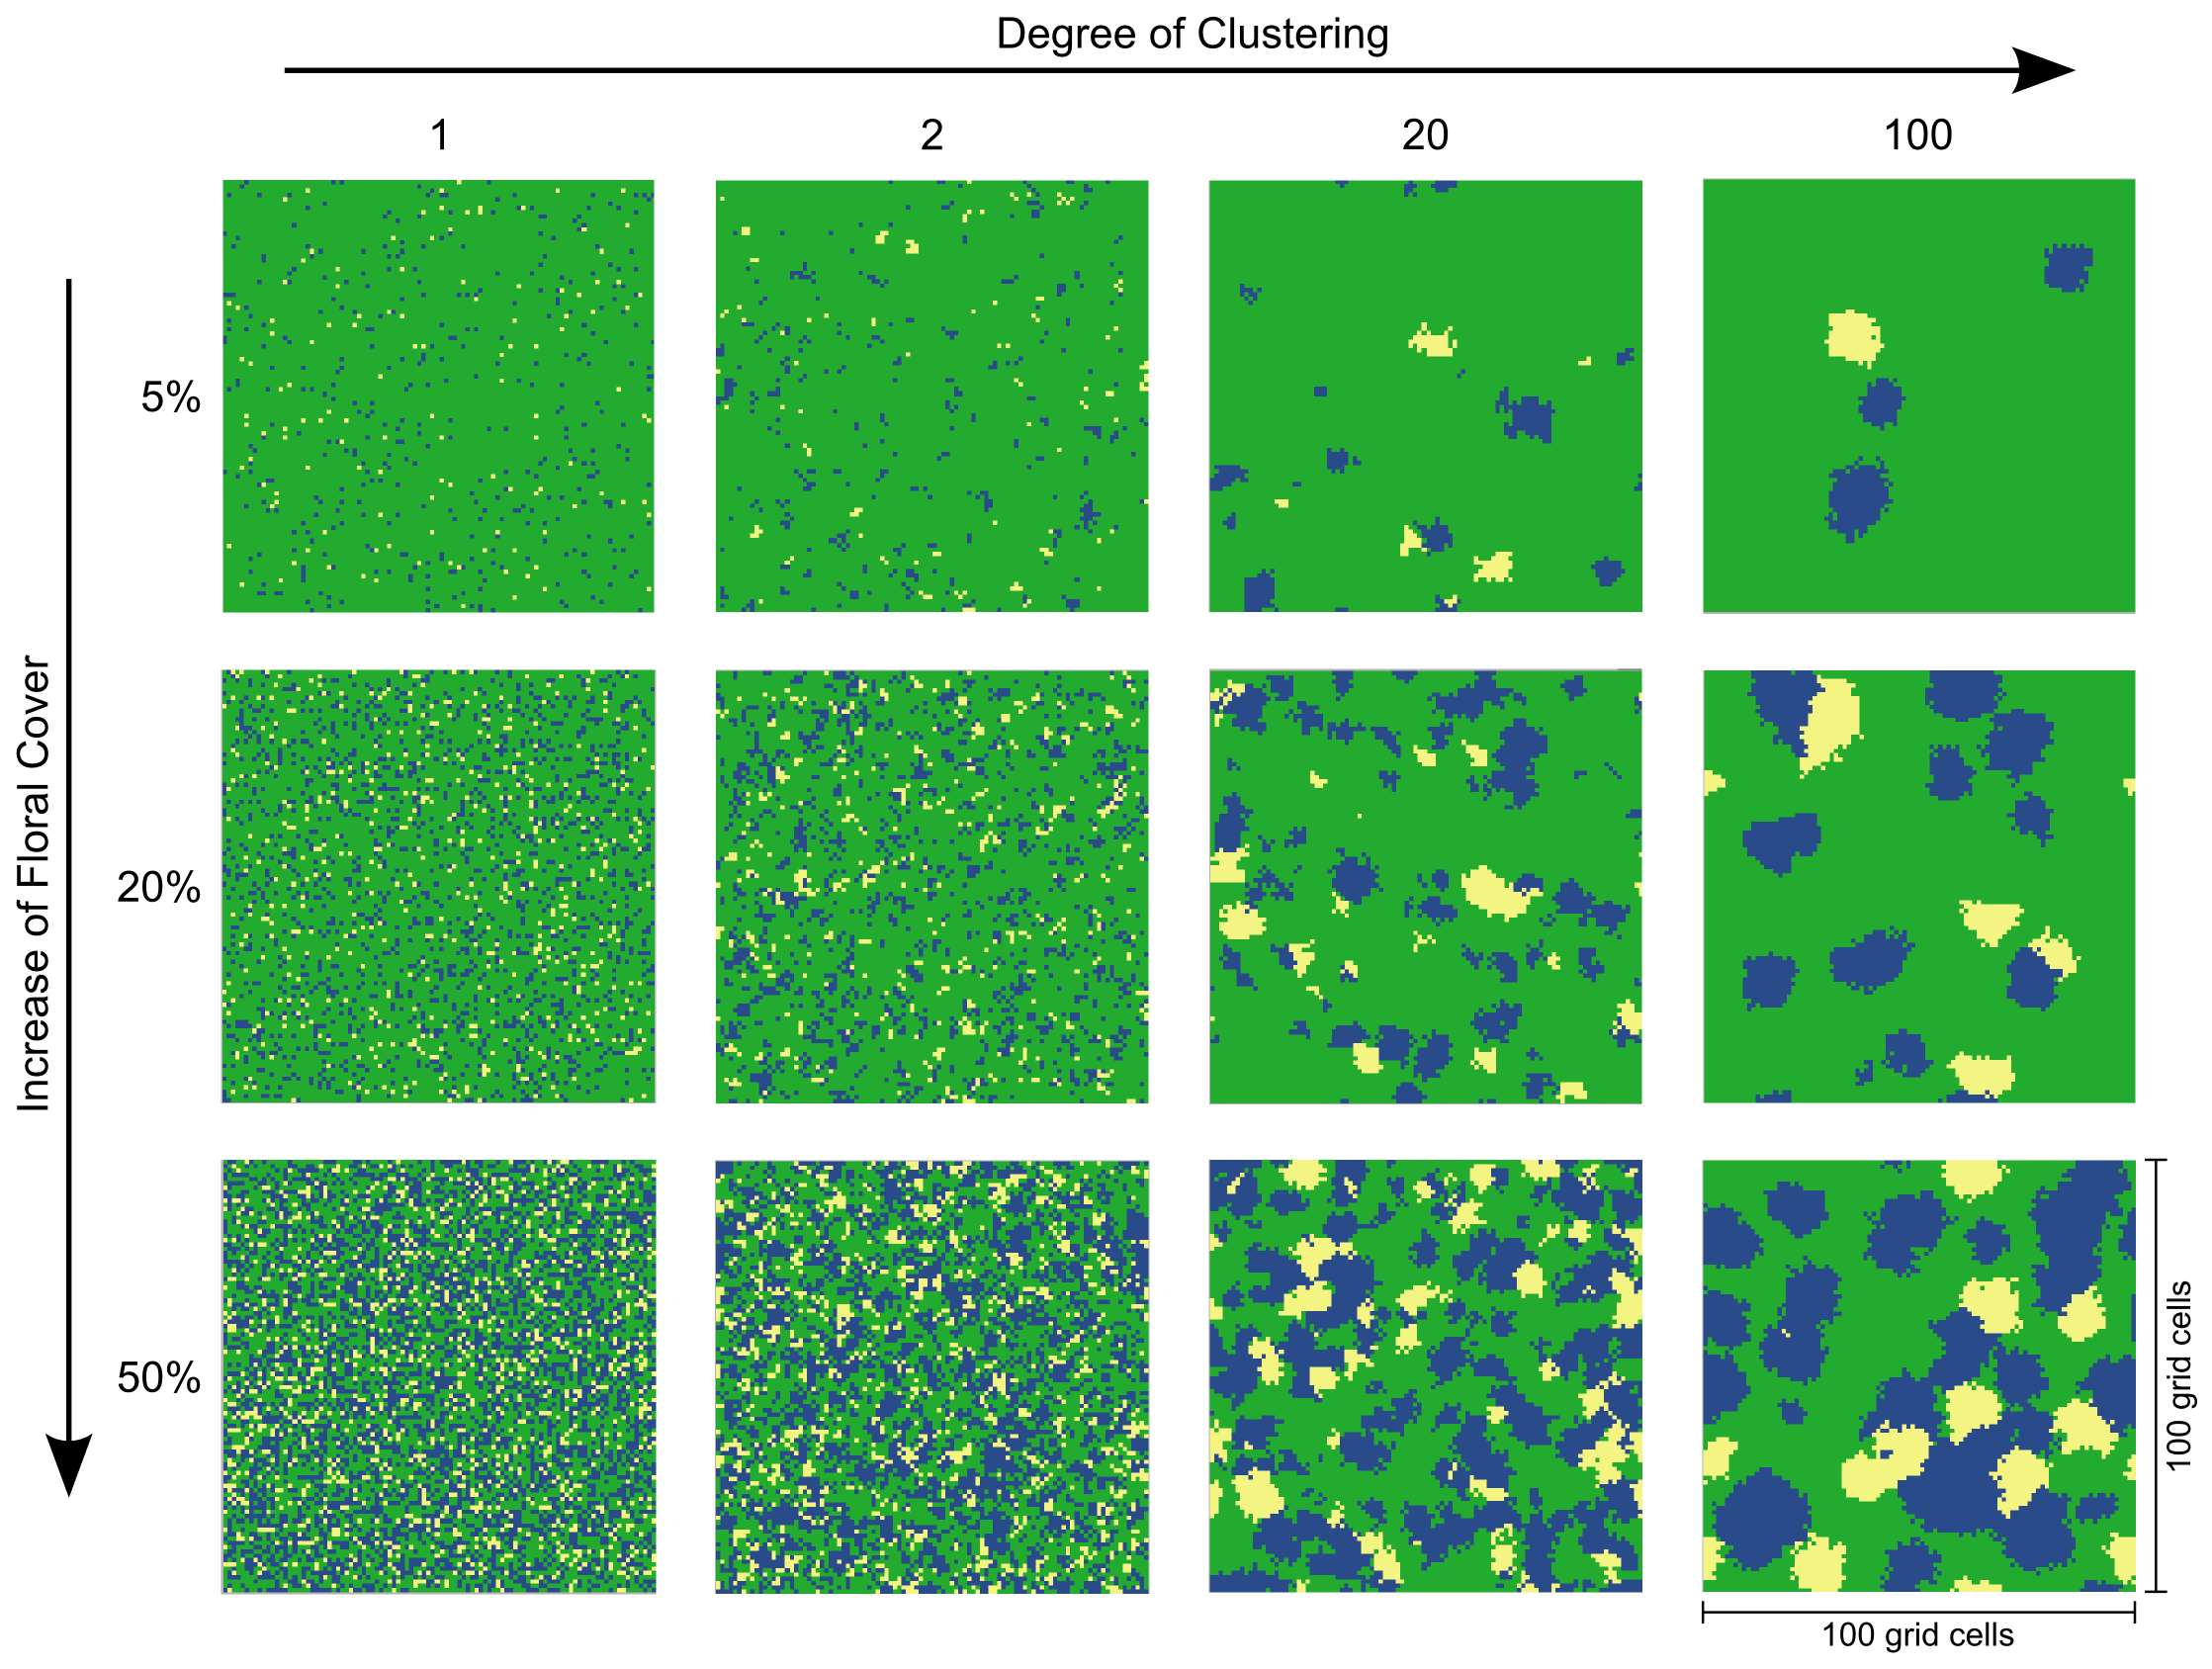
\includegraphics[width=14cm]{Images/cluster}
	\caption{ Exemplary model environment setups with increasing floral cover and cluster size. The cover expresses the percentage of patches containing a flower ($\Sigma_{patches}$ = 10 000). The cluster number equals the average amount of flowers per cluster. Flowers are randomly assigned to the clusters in the model setup. }
	\label{fig:cluster}
\end{figure}


\subsection*{Behavior Rules}

All bee-agents act independently from each other according to the behavior rules shown in Figure~\ref{fig:flowchart} (Overview of all parameters used for the model with its default settings in the supplementary material in tab.~\ref{tab:parametervalues}).  

As mentioned in the assumptions, the behavior of the bee-agents is strongly influences by flower constancy ( e.g. \citealp{bobisud1975pollinator, chittka1997foraging, thomson1981field, chittka1999flower,  goulson1994model,  goulson1999foraging}). Bee-agents always prefer of one of the two flowering species and forage exclusively on this species. The preference can change due to lack of searching success or a series of low rewards of the preferred flower \citep{chittka1997foraging,kunin1993sex,greggers1993memory}. At any given time, a bee-agent can be in one of two states: search for a flower or visit one. 


\begin{figure} [!ht] %flowchart
	\centering
	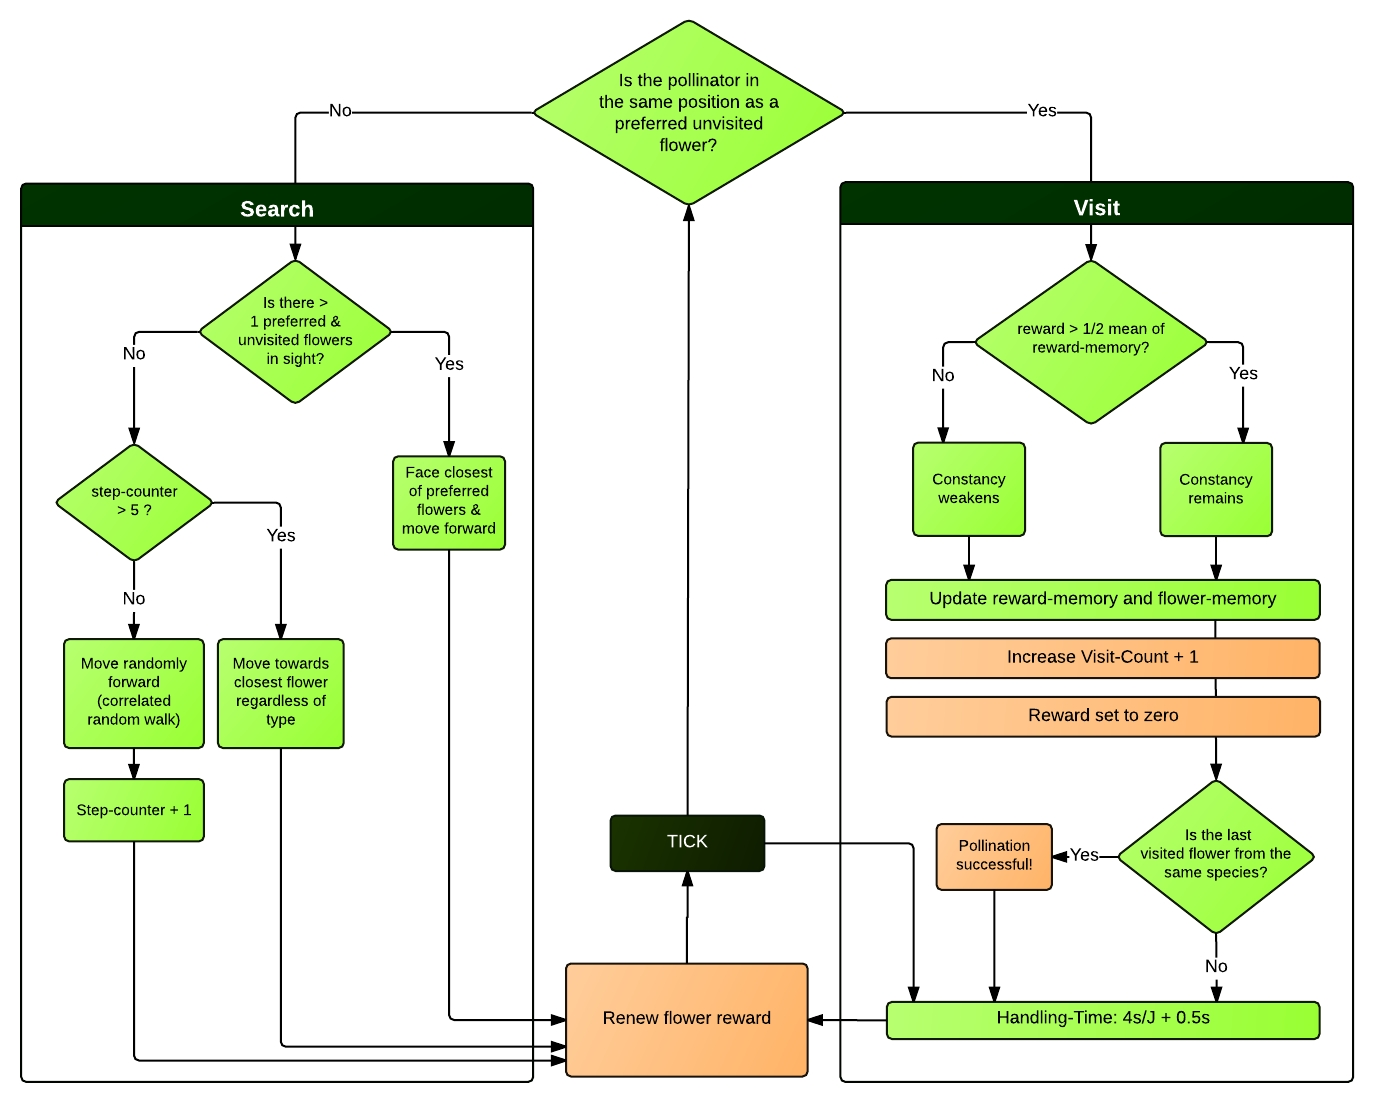
\includegraphics[width=14cm]{Images/flowchart-model}
	\caption{Flowchart describing the behavior rules for the bee-agents within the agent-based model. At any time given, a bee-agent can either search for a preferred flower or visit one. While searching, a bee-agent can remember the location of the last four visited flowers to avoid double-encountering. If there is no flower in sight after 5 seconds of correlated random walk (CRW), the probability that it will encounter the next available flower despite its type increases by 10\% per additional time step. When a bee-agent visits a flower it takes all reward within a reward-dependent handling time and compares the amount with its memory. If the reward is low, the agent is more likely to visit the other flower type next time. The maximum of visits within a successful pollination is possible (x) is determined by the pollen carryover parameter.}
	\label{fig:flowchart}
\end{figure}


\subsubsection*{Search}

Pollinators avoid recently visited flowers \citep{goulson1999foraging}. Every bee-agent possesses with a memory to remember the location of the last four already visited flowers \citep{goulson2000pollinators}. 
 If there is any not recently visited and preferred flower in sight, the searching bee-agent moves directly towards the flower, otherwise it continues searching. 

Previous research on the speed of foraging pollinators by \cite{essenberg2012explaining} and \cite{kunin1991few} (in  \citealt{kunin1996pollinator}) gives 0.1m/sec as benchmark. Consequently, bee-agents can move 1 grid cell per time step in this model. The vision of pollinators was studied in various experiments using a Y-maze apparatus \citep{dyer2008comparative, wertlen2008detection, ne2001effect}. Every bee-agent can detect flowers from a distance of 0.7m with an equivalent of 6 grid cells. The vision is reduced to a 180$^{\circ}$ cone-shaped field to the front of the agent. Pollinators tend to keep their direction while foraging \citep{waddington1980flight}. In the model, I used a correlated random walk (CRW) to achieve a relatively natural movement \citep{bartumeus2005animal, codling2008random,  pyke1992flight, viswanathan2008levy}. Empirical studies have shown an increasing probability to abandon the original flower preference the longer the search remains unsuccessful \citep{chittka1997foraging,kunin1993sex}. If the bee-agent searches for 5 seconds (= 5 time steps) without finding any preferred and unvisited flower, the likelihood of changing its preference increases by 10\% with every additional time step. \\

\subsubsection*{Visit and Reward Intake}

When a bee-agent encounters a preferred and unvisited flower it takes up all its reward. As long as the reward content of a flower lower than the maximum it is refilled by 0.00004 Joule in each time step until the maximum of 1 Joule is reached (see "reward-function" in tab.~\ref{tab:parametervalues}). The handling time of a bee-agent visiting a flower involves three components: a time proportional to the amount of reward taken, a reward-independent constant and a skill factor \citep{kunin1996pollinator}. In my model, a bee-agent requires 4 seconds to extract one Joule of reward plus a reward-independent handling time of 0.5 seconds. When the bee-agent just changed its flower preference it gets a 3 second penalty for inexperience (\citealt{roubik1992ecology}, \citealt{kunin1996pollinator}).

The reward taken is stored in each individual's reward-memory. Every agent can remember the last four rewards received. When visiting a flower, the bee-agent compares this memory with the current reward quantity. If the reward is less than half the average in the memory, the likelihood to abandon flower constancy and visit the other species next increases by 10\%. If the reward is exceptionally good (at least twice the remembered average), the change probability is set to zero  \citep{chittka1997foraging, keasar1996innate}. 

Additional to the quantity of visits we're also interested in their quality. A flower can only be successfully pollinated if the bee-agent visited the same species before. The maximal number of heterospecific flower visits which still allows successful pollination is determined by the degree of pollen carryover. The parameter applies to all bee-agents and can have a value between 1 and 16. For the value of one, the very last visit has to be from the same species (strong heterospecific pollen interference, see \citealt{campbell1986predicting,benadi2012population,montgomery2009pollen}).

After reward-collection is completed, the bee-agent updates its flower-memory and its reward-memory and continues foraging. Each visit and successful pollination is recorded for later analysis. 


\subsection*{Simulation experiments}

Parameters altered in the main analysis are frequency, floral cover, degree of clustering and pollen-carryover. Each parameter-combination was run 20 times with a length of 1000 ticks each (110,400 runs in total). Additionally, I performed a sensitivity analysis with additional parameters which affect the behavior of the bee-agents to understand how the values of these parameters influence the frequency dependence of per-flower visitation rate. Table~\ref{tab:simulation_run} presents the definition and value range of the parameters.
 
\begin{table} [!htbp] %parameter values
	\centering
	\caption{Parameter values used for the main and sensitivity analysis. Only general parameters were changed in the main analysis, whereas the sensitivity analysis also directly influences the behavior of the bee-agents. Each combination was repeated 20 times for 1000 time steps, that makes a total of 110,400 runs in the main analysis and 16,560 runs for each parameter of the sensitivity analysis. }
	\begin{tabular} {l l l}
		\toprule
		\textbf{Parameter} & \textbf{Description}  & \textbf{Values}\\
		\midrule
		\addlinespace[0.2cm]
		\multicolumn{ 3} {l} {\textsc{Main analysis}} \\ 
		\addlinespace[0.2cm]
		Frequency & Proportion of species A on all flowers  & 0-100\% (5\%-steps)\\
		Flower cover & Proportion of patches containing a flowers  & 5, 10, 20, 50 \%\\
		Degree of clustering & Average number of flowers per cluster   &  1, 2, 5, 10, 20, 50, 75, 100\\
		Pollen carryover & Number of visits within a successful pollination is possible & 1, 2, 4, 6, 8, 16\\
		
		\addlinespace[0.2cm]
		\multicolumn{ 3 } {l} {\textsc{Sensitivity analysis}} \\ 
		\addlinespace[0.2cm]
		Reward function & Increase of reward per flower and second & 0, 0.00004, 0.001, 0.1 J/sec \\
		Vision distance & Range of patches within a bee-agent can detect flowers & 1, 6, 20, 50 patches\\
		Search time & \begin{tabular}{@{}l@{}} Number of seconds a bee-agent searches before\\ the probability of switching flowers increases \end{tabular}   & 1, 5, 20, 50 sec \\
		Pollinator density & Number of bee-agents on the meadow & 5, 10, 20, 50 bees\\
		
		\bottomrule
	\end{tabular}
	\label{tab:simulation_run}
\end{table}


%1414 words
\newpage

\label{ch:results_model}

\subsection{Results}

\subsubsection*{Per-flower Visitation Rate}

\begin{figure} [!ht] %results:PFV
	\centering
	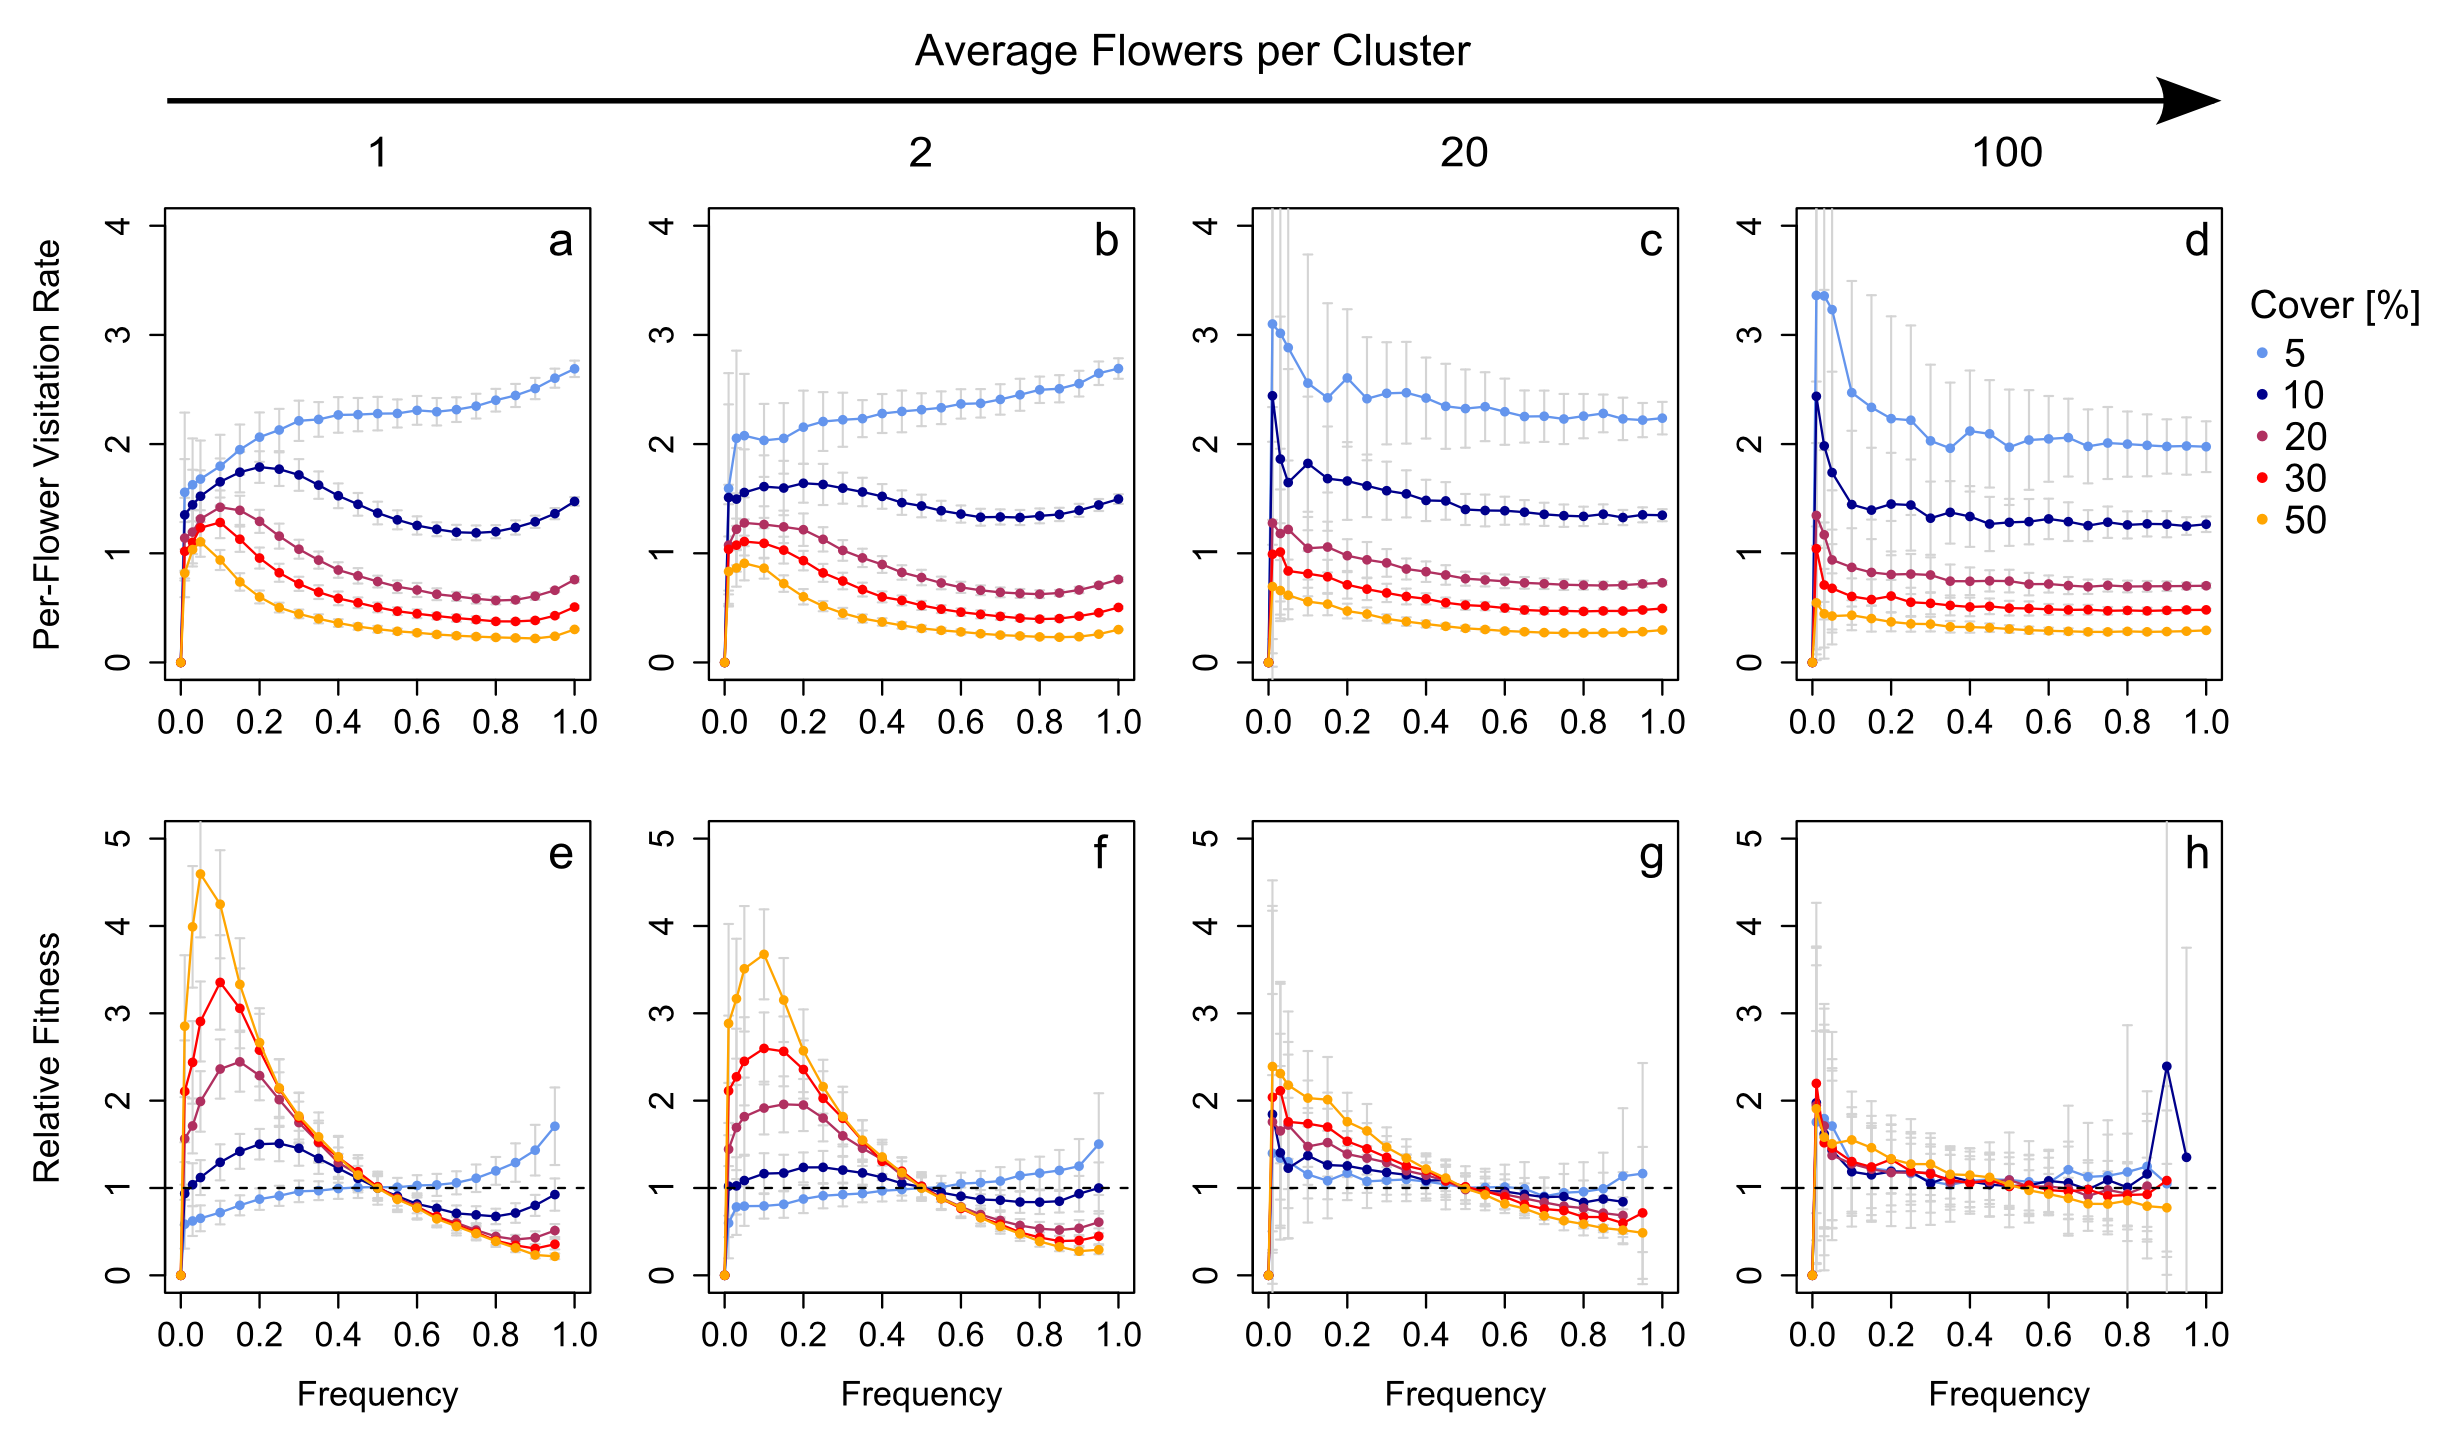
\includegraphics[width=16cm]{Images/PFV}
	\caption{The per-flower visitation rate shows a frequency dependence with a cubic relationship. The same data is plotted relative to per-flower visitation of the other species to visualize the relative fitness and intensity of frequency dependence (e-h). A value of one means no benefit in visits per flower for either species. The frequency effect is stronger for higher floral cover while an increase in cluster size reduces the frequency dependence. The peak at 90\% for 10\% cover in a 100 flowers per cluster environment is due to a statistical outlier highly influencing the mean. The parameter combination was run again for validation (supplementary material, Fig.~\ref{fig:outlier}). Note that the statistical variability increases for very low frequencies in highly clustered scenarios (grey error bars). If a rare species is occurring only in one cluster on the meadow, it will receive either no or multiple visits. See Fig.~\ref{fig:PFVgross} in the supplementary material for an enlarged image.}
	\label{fig:PFV}
\end{figure}


The per-flower visitation shows for small clusters a similar cubic function as the data collected in the Jena Experiment (Fig.~\ref{fig:PFV}a,b). Within the first 20\% there is a steep increase in visits per flower. Afterwards, since for all cover values above 5\% the additional gain of visits is not proportional to the increase of flowers due to higher frequency, the per-flower visitation drops with a minimum around 80\%. Close to 100\%, when the species becomes dominant, the per-flower visitation rises again. Cover and cluster size both influence the frequency dependence. The higher the cover, the lower the per-flower visitation and the bigger the clusters the less visible is the frequency dependence. Simulations with more than 10 flowers per cluster show a high variance for frequencies below 10\% and very low to no frequency dependence afterwards (Fig.~\ref{fig:PFV}c,d). 

The same data is plotted as relative visitation rate to see which species has a higher fitness and to take the variance in the sum of visits into account (Fig.~\ref{fig:PFV}e-h; see section "Global visitation"). If the value is one, both species receive the same per-flower visitation. For 5\% cover, the bee-agent exhibits a positive frequency dependence. If the cover is higher, the rare species benefits from a negative frequency dependence. Cluster size reduces the effect and the data approach a slightly negative frequency dependence (Fig.~\ref{fig:PFV}h). 

\subsubsection*{Pollination Success}

\begin{figure} [!ht] %results:POC
	\centering
	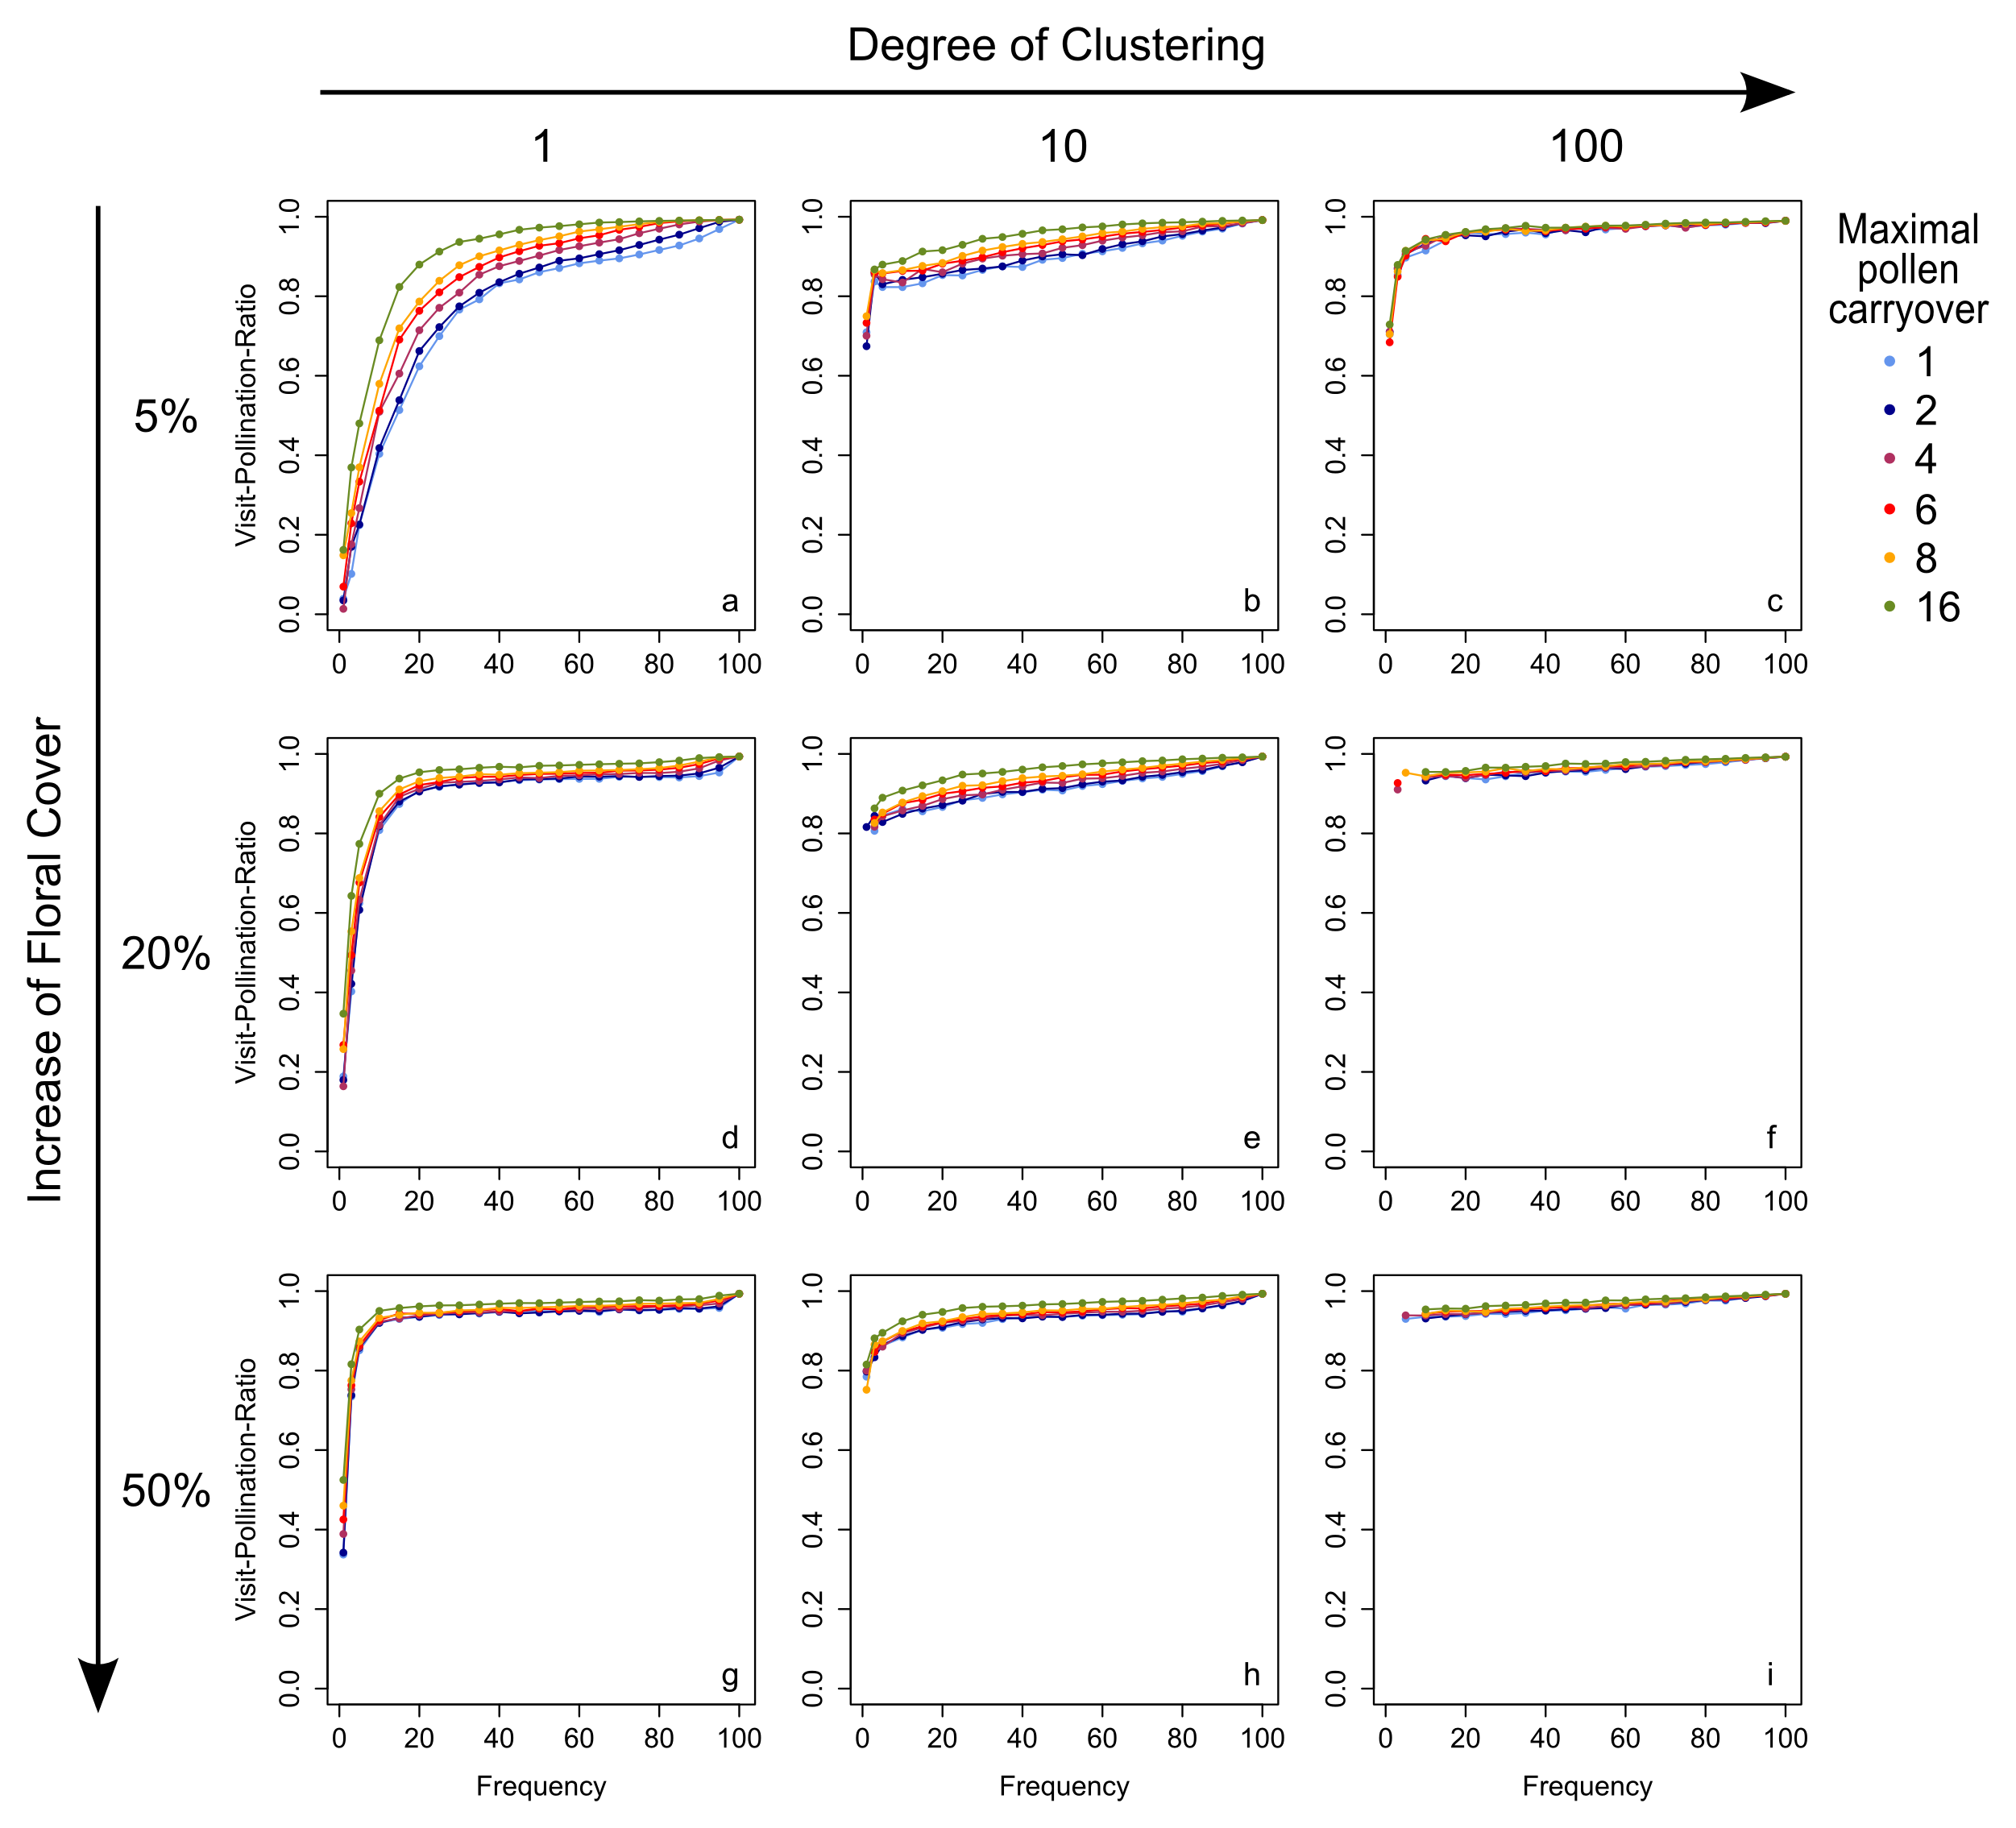
\includegraphics[width=15cm]{Images/POC}
	\caption{Frequency dependence of proportion of successful pollinator visits for different combinations of floral cover and cluster size. The pollen carryover value defines the maximum number of heterospecific visits within a successful pollination is possible. With a pollen-carryover rate of one, the pollen can only be carried to the next flower. Therefore, the ratio of successful pollinations per visit can be seen as indicator for flower constancy \citep{montgomery2009pollen}. A high pollen-carryover rate is only important for a low cover and no-cluster environment. With increasing cover and cluster, the ratio becomes steeper for low frequencies which stands for more qualitative visits.}
	\label{fig:POC}
\end{figure}

The degree of pollen carryover is defined as maximum number of heterospecific visits within a successful pollination can take place. In the model, I tested values from 1 (strong heterospecific pollen interference) to 16 (weak heterospecific pollen interference). Figure~\ref{fig:POC} gives the proportion of all visits where a successful pollination took place. The first 20\% frequency are crucial for all parameter-value combination. A very steep increase up to 80\% successful visits is followed by a moderate linear increase up to 100\% for exclusive existence. The degree of pollen carryover only makes a difference for small cover and cluster values (Fig.~\ref{fig:POC}a). The higher the cover and the bigger the clusters, the better is also the proportion of successful pollination, even for small frequencies, independent of the pollen-carryover rate(Fig.~\ref{fig:POC}c,f,g-i). 

\subsubsection*{Global visitation}

\begin{figure} [!ht] %results:SUM
	\centering
	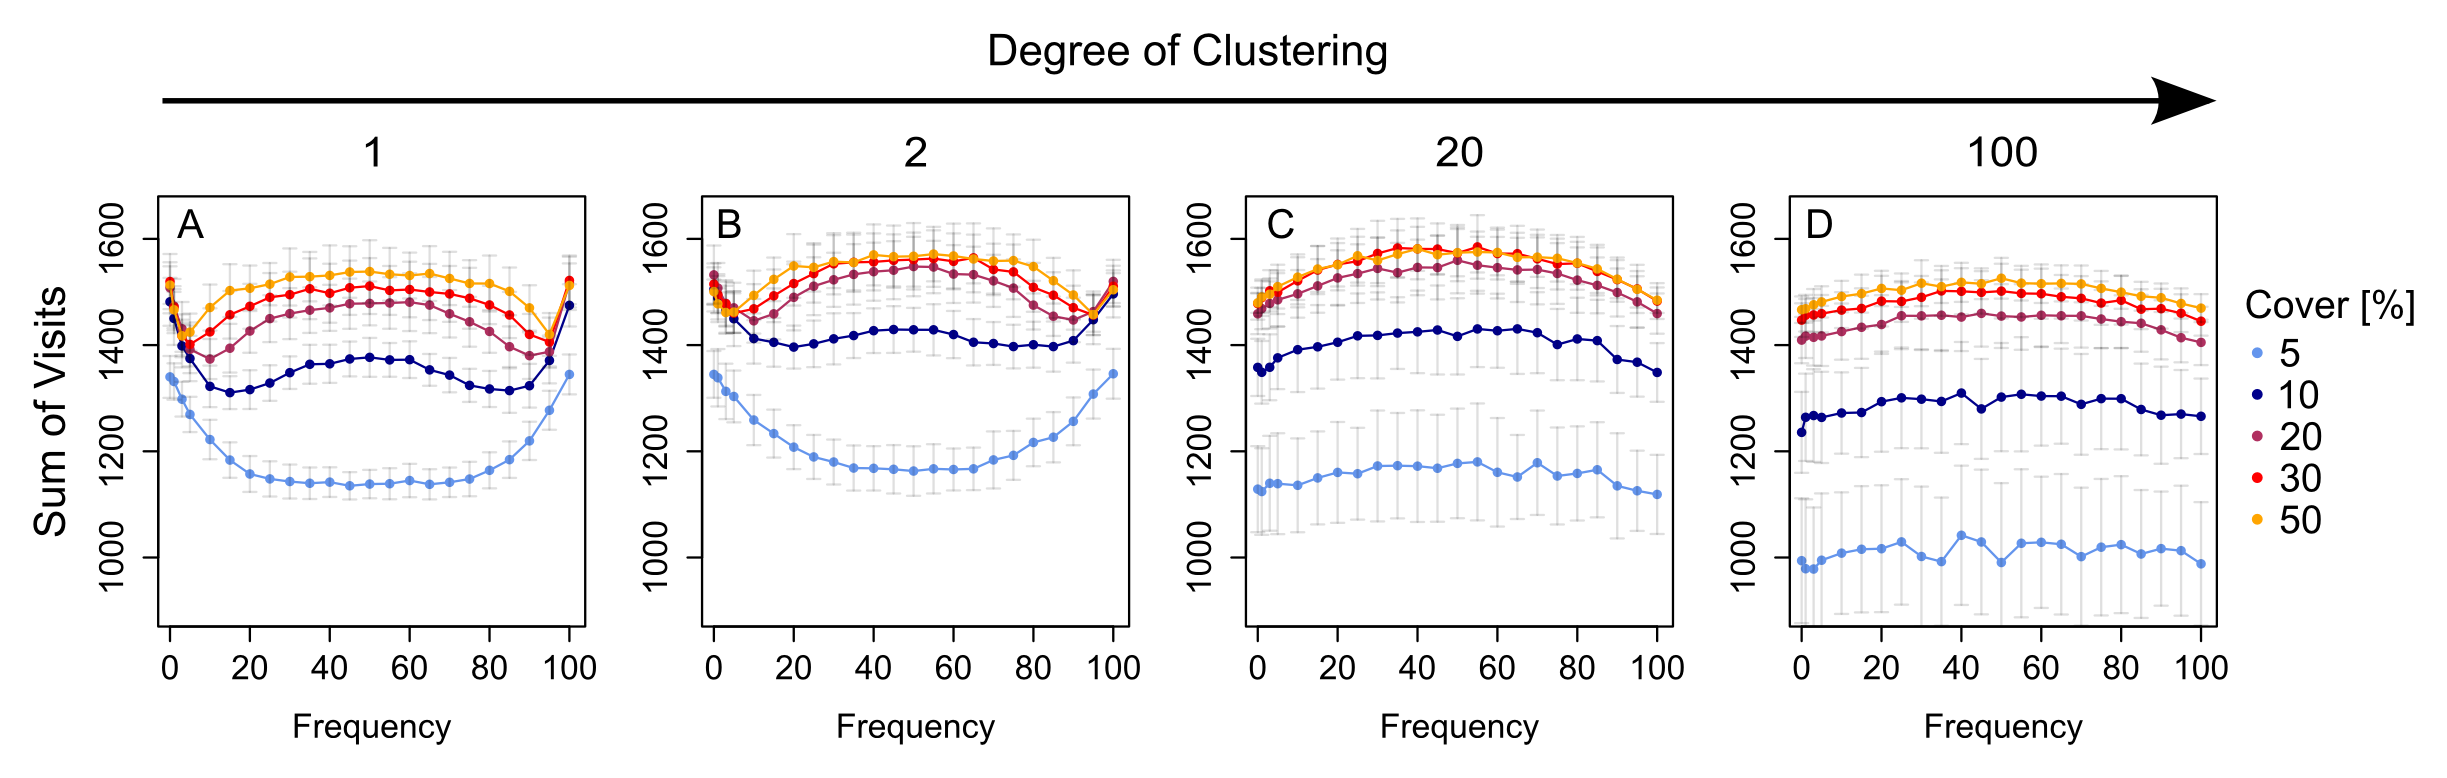
\includegraphics[width=16cm]{Images/SUM}
	\caption{Summed visits to both species show a frequency dependence for low cluster values. Depending on the floral cover it is quadratic or a fourth-degree polynomial relationship. The maximum number of visits (maximal efficiency) is achieved for highly unequal or balanced frequencies of the two plant species, depending on floral cover and cluster size.}
	\label{fig:SUM}
\end{figure}

The sum of all visits to both plants together changes with the ratio of their abundance (Fig.~\ref{fig:SUM}). A strong cover-dependent pattern is visible for small cluster sizes. The total visits have an u-shaped relationship with frequency for 5\% cover and a shape similar to a fourth-degree polynomial function for higher cover values. The visitation drops to a minimum at 90:10 ratio and peaks again for balanced frequencies. Cluster size reduces the frequency dependence. \\
Note that the mean number of total visits varies in addition to the shape for different values of cover and cluster size. Both parameters have a frequency independent influence on the visitation rate (Supplementary material, Fig.~\ref{fig:nonfreq}). Floral cover shows a saturated curve and the visits for degree of clustering have a hump-shaped relationship with a peak at an intermediate aggregation level of 5-10 flowers per cluster.

\subsection*{Sensitivity Analysis}
Aim of the sensitivity analysis is to understand influence of behavioral rules on the outcome of the model. Therefore, pollinator density, reward regrowth, search time and vision were tested for a (unnaturally) broad range of values set in comparison to the empirically founded default values. Vision, search time and the number of bees on the meadow influence the sum of visits (Fig.~\ref{fig:SA_SUM}). A larger range of vision leads to more visits, the search limit reduces the number of visits and more bees lead again to more visits per time unit. The reward function has an small negative influence on the total number of visits for a very high regrowth rate.

Furthermore, a very high replenishment rate (0.1J/sec, yellow line in Fig.~\ref{fig:SA_reward}) has a reversing effect on the frequency dependence: Rare species receive disproportionally few visits whereas common species benefit from a positive frequency dependence. The influence of frequency is less severe with increasing cluster size. 

Every bee-agent can detect flowers in a 180$^{\circ}$ cone-shaped array of patches in front of them. The number of patches in that array is determined by the vision distance. A large range of vision increases the frequency dependence even in a heavily clustered model environment (Fig.~\ref{fig:SA_view}). If the bee-agents are only able to see the direct neighbor, the frequency dependence is reversed to favor the common species for low cluster values. 

If a bee-agent searches longer than a given search time limit unsuccessfully for a unvisited and preferred flower, the probability to switch preferences will increase by 10\% with every additional step. The search limit was altered from 1 to 50 seconds in the sensitivity analysis. The results are similar to the effect of vision as they also change the probability to switch preferences. Higher search time limits lead to stronger negative frequency dependence benefiting the rare species. A search limit of 1 second reduces the dependency (Fig.~\ref{fig:SA_flight}).

Beside the expected increase of absolute visits, a change of pollinator density has no effect on the outcome of the model at any cover or cluster values (Fig.~\ref{fig:SA_bees}).


%%%REWARD
% Hence, a high reward can fix decrease diversity
% with very high reward rates, the bees find rarely a flower with bad reward and are changing preference less often. The only other way of changing preference is unsuccessful flight and that favors the common species
%IMPORTANT! Explained all lab experiments dome by smithson et al 1997a,1997b & 1996

%%VIEW
%with high vision bee-agents are able to detect flowers of the rare species more quickly and are less likely to change their preference
%similar result as changing search time limit or make density higher
%if the bee can see further it will fly more directly to the next flower without too much random walk. but on the other hand it will fly for longer distances instead of changing preference to the more abundant species. Less efficient, less total visits

%%%FLIGHT
%with higher search time limit, the bee continues to search for the rare species instead of changing to the more abundant species. That is less efficient (less absolut visits) and enhances the FD
%850 words
\newpage

\label{ch:discussion}
\section{Discussion}
Frequency dependence can influence the plants fitness and therefore have far reaching consequences for the development and maintenance of biodiversity. Aim of this thesis is to study the existence of frequency dependence in a natural plant community, explore the kind of relationship and identify the factors influencing frequency dependence with the help of an agent-based model.\\
I found evidence for frequency dependent pollination for rewarding flower species in grassland plant communities in the field data. The relationship is defined by a steep increase of visits within the first 20\% frequency followed by a disproportional low gain of visits for every additional flower due to an increase of frequency. When the species becomes dominant the per-flower visitation rate increases again. The combination of negative and positive frequency dependence combined in a cubic curve is generally supported by the agent-based model. Furthermore, the model reveals floral cover and cluster size as important influencing factors for frequency dependence. \\


Previous research found positive frequency dependence for lab experiments on rewarding flowers and inconsistence in the few field experiments focusing on color morphs \citep{smithson2001pollinator}. However, the field data shows a cubic pattern of frequency dependency for at least four different rewarding flower species and the results from the foraging simulation support the general shape of the per-flower visitation ratio. Where does the discrepancy of lab and field data comes from?\\ 

The sensitivity analysis of the agent-based model can give an explanation: If the reward function is increased to a refill within 10 time steps, the relationship is reversed to a positive frequency dependence and the rare species receives disproportionally few visits (Fig.~\ref{fig:SA_reward}). The curve is consistent with findings of  \cite{smithson1997density} and \cite{smithson1996frequency}. In their study design, artificial flowers were refilled after each foraging bout. Therefore, every bumble bee foraged on a set of full and equally rewarding flowers which is comparable to a high regrowth function in the agent-based model.\\
We know that pollinators more likely abandon flower constancy if they experience sequentially bad reward \citep{chittka1997foraging,goulson1994model}. If the reward is always high, pollinators have less incentive to go on exploratory visits to the rare species as the abundant type is easy to find and sufficient rewarding. Hence it can be assumed that negative frequency dependent selection does not exclusively apply for non-rewarding species but also for flowering communities with varying or insufficient reward. Strong positive frequency dependence in pollination might be only possible for highly rewarding or artificial systems. 

%More research, especially on natural field conditions, is needed to confirm this hypothesis.

%high nectar production rates increases approach rates Pleasants 1981; Real & Rathcke 1991;Duffield al 1993; Shykoff & Bucheli 1995 (from  Klinkhamer 2001)

\subsubsection*{Floral cover and cluster size are influencing factors}
The model reveals two main influences for frequency dependence: The higher the floral cover, the stronger the frequency dependence and the bigger the clusters, the weaker the frequency dependence (Fig.~\ref{fig:PFV}e-h). 
Floral density is known to influence visitation rates, usually positive and with a saturating function (eg. \citealt{rathcke1983competition,essenberg2012explaining,bernhardt2008effects,Kunin1997}). Those findings are consistent with the Holling´s type II functional response found for different cover values (Supplementary material, Fig.~\ref{fig:nonfreq}a). If the cover is increasing, the absolute number of flowers rises also for the rare species. That makes it more likely for a bee-agent to find a flower before changing preference towards the common species due to long search times even if foraging on the later would be more efficient. Therefore, high cover causes the same effect as expanded vision distance or maximum search limit (cf. Fig.~\ref{fig:SA_view} and Fig.~\ref{fig:SA_flight}): The main reason of abandoning flower constancy becomes multiple visit of flowers with low reward. Consequence are explanatory visits to the rare species which can have a great impact on the per-flower visitation rate. Every visit to a rare species weights high in the per-flower visitation rate because the sum of visits is divided through the number of flowers.\\ 

The model shows that spatial aggregation of flowers can lead to a more efficient foraging (more visits per time unit), less frequency dependence and a higher quality of visits due to compatible pollen deposits. If flowers are randomly distributed over the whole meadow, many short search and flight times apply. An intermediate cluster level is easy to exploit by a pollinator whereas the flight and search times can be very long in between few big clusters, especially for low floral densities. \\
It was already suggested by \cite{epperson1987frequency} that spatial agglomeration of flowers decreases frequency dependence. In the agent-based model, a similar effect compared to low cover takes place: If flowers are aggregated at few places, they affect the pollinators perception of frequency and are more difficult to find. Long search times will weaken the bee-agents flower preference and lead to foraging on the next available cluster independent of its species. 

%more literature!

\subsubsection*{Requirements for successful pollination}
High visitation rate is gained at low frequency with high cover and low cluster size. However, those visits might not be the best quality if the pollination per visit ratio is comparatively low (Fig.~\ref{fig:POC}a,d). The ratio can be seen as index for flower constancy: If the majority of visits lead even for a small pollen carryover value to successful pollination the bee-agents forage very flower constant \citep{montgomery2009pollen}. If the cover is high, bee-agents will keep their constancy also for rare species because they are abundant enough. If the aggregation of flowers is high, bee-agents exploit this cluster before leaving for the next. Every visit within a cluster of flowers of the same species is counted as successful pollination and can lead to a high visit quality even if the cover is low (cf. \citealt{jakobsson2009relationships}). Therefore, rare species should occur in clusters of flowers if the cover is low to get a maximum of pollination per visit. If the cover is high the spatial distribution plays a minor role for the visit quality.  

%vgl Hanoteux?
%see Feldmann 2008

\subsubsection*{Sum of visits to the flower community also show frequency dependence}
Additionally to individual frequency dependence, I analyzed the impact of species partitioning on frequency dependent visitation in the system as whole. \\
If the cover is very low, a maximum in total visits can be received if one species is dominant. Co-flowering will lead to longer search times and less overall visits (u-shape for 5\% cover in Fig.~\ref{fig:SUM}a). For higher cover, the frequency dependence shows a function similar to a fourth-degree polynomial. If one species is rare at 5-20\% frequency, pollinators exhibit exploratory visits to the rare species and spend inefficient time searching. Hence, the total visitation number drops to a minimum. If species are evenly distributed the pollinators forage on both species in equal amounts. This is the most efficient status for the overall ecosystem, especially for high cover or cluster size. \\
Spatial aggregation weakens the frequency effect but will also reduce the total visits. If flowers are even and random distributed, the bee-agent has many small search times intermittent by collecting reward on a single flower and continue foraging. Rare flowers can be found comparatively easy if they are spread over the whole meadow and flower constancy will be kept even if it is highly inefficient. If the clusters of flowers are bigger, bee-agents will not find rare flowers that easily because they might occur only in a single cluster on the meadow. The bee-agent switches to the common flower, the minimum at very uneven distribution disappears and the relationship becomes slightly hump-shaped (Fig.~\ref{fig:SUM}b,c). \\
A maximum of overall visits favoring both the pollinators and the co-flowering plants can be achieved with balanced abundance in high cover and very uneven species distribution for low floral cover environments. 

\subsubsection*{Limitations of the study design and research suggestions}
Even though modeling can be an excellent tool to understand and interpret ecological data, some questions evolve comparing the data collected in the Jena Experiment and the foraging model. Floral cover is an important factor in the outcome of the model. It influences not only the absolute number of visits but also the intensity of frequency dependence. But it was removed in the model selection as it was no factor of explanatory power to the per-flower visitation data. 
Reason could lie in the sampling design. Data was only observed from plots with an intermediate cover, no extremes were taken into account. In total, there were only five values for cover in the final analysis. Also all cover values are estimations, no exact measurements. Also, pollinators are influences by many factors in the field, not all of them measured in this study or possible to take into account at all. Other floral traits like scent, the pollinators detection of colors and differences in pollinator types are just some factors which might have an impact on the foraging behavior and consequently also on frequency dependence. \citep{smithson2001pollinator}. \\

Validation of further results of the agent-based model can be made via a supplementary study with varying frequency, cover and cluster size of two co-flowering species. Practical is a simplified study design with less influencing variables either under natural conditions where manipulation is possible (eg. \citealt{Eckhart2006frequency,essenberg2012explaining}) or with potted plants \citep{epperson1987frequency}. Also results of the frequency dependent sum of visits could be tested by manipulated field experiments. Natural conditions data are not suitable for this purpose because every plot contains more than two co-flowering species with unequal attractiveness.  
The data collected in Jena shows drastic differences in attractiveness of the focal species and frequency dependence was found to be subject to each species. Therefore I suggest continuous research on a variety of species, both rewarding and unrewarding with measurements of reward to check if my findings are universally valid.\\

%1518 words

\section{Conclusions}
\label{ch:conclusions}
In conclusion, this study shows for the first time that frequency dependent selection exists in natural flowering communities for a broad range of flowers, not only for color morphs. Also, a combination of methods is exceptionally helpful to understand underlying drivers. The output of the agent-based foraging model confirms the results of the field data and fills the knowledge gap of previous research: Positive frequency dependence proved multiple times in lab experiments is likely due to very high rewards. Negative frequency dependence is therefore not exclusive to non-rewarding morphs but takes effect also for common rewarding species if the reward is not exceptionally high. Patterns of frequency dependence can therefore change across space and time, especially because the model revealed floral cover as FD-increasing and agglomeration of flowers FD-reducing factor.

Those findings are important for our understanding of the evolution and conservation of diversity. Negative FD, thus if rare flowers have an advantage in pollinator visits, might be an important factor in the evolution not only floral polymorphisms but diversity as such. 

Further research is necessary to validate the role of floral cover and cluster for FD. A controlled field experiments including measurements of floral reward and pollination success could be a suitable approach. Based on the findings, I also recommend the connection of modeling, field and lab work. Most research is only done in one of those three approaches, cross-validation is often missing completely. It could be gained a great deal of knowledge by establishing interdisciplinary working groups of field ecologists and environmental modeling experts. \\

What else? (Nor yet included)
\begin{itemize}
	\item POC
	\item Best for ecosystem and bees (most visits, most efficiency): extreme or balanced frequency, high cover, intermediate cluster
\end{itemize}

% 258words

\newpage

\bibliographystyle{apalike}
\bibliography{masterthesis1}

\newpage

%\label{ch:appendix_jena}

\section{Appendix}

\subsection{Jena}

\begin{table}[!htbp]
\centering
  \caption{Per-flower visitation rates (mean $\pm$ SD) for all focal flower species per 15 minute observation. \textit{Geranium pratense} and \textit{Onobrychis viciifolia} are significantly different from the other three species (pairwise t-test, \textit{p} $<$ 0.001) . Within the two groups, there is no significant difference between the species. }
    \begin{tabular}{l l l l l}
    \toprule
    \textbf {Short} & \textbf{Species} & \textbf{Family} &\textbf{Visitation Rate (Mean)} & \textbf{ $\pm$ SD} \\
    \midrule
    Ger  & \textit{Geranium pratense} & Geraniaceae & 3.05 & 1.5 \\ %109
    Lat  & \textit{Lathyrus pratensis} & Fabaceae & 0.57 & 0.53 \\ %83
    Lot  & \textit{Lotus corniculatus} & Fabaceae & 0.30 & 0.36 \\  % 77
    Ono  & \textit{Onobrychis viciifolia} & Fabaceae & 3.60  &  2.5 \\ % 37
    TP   & \textit{Trifolium pratense} & Fabaceae & 0.16 & 0.23 \\ % 79
    \bottomrule
    \end{tabular}%
\label{tab:VR_spec}
\end{table}%

%%%%%%%%%%%%%%%%%%%%%%%%%%

\begin{table} [!htbp] %results lme
	\centering
	\caption{Results of the linear mixed effect model with per-flower visitation rate as explanatory variable. Floral cover and species richness were not relevant predictors for the model and therefore removed in the model selection process (denDF = 191, R$^{2}$ = 0.53, n = 385)}
	\begin{tabular} { l l c c c}
		\toprule
		\textbf{Response Variable} & \textbf{Explanatory Variables} & \textbf{Df} & \textbf{F-value} & \textbf{\textit{P}} \\
		\midrule
		Per-flower visitation rate   & Species & $4$ & $130.9$ & $<0.0001$\\
		& Frequency 			&  $1$ & $49.3$ & $<0.0001$ \\
		& Frequency$^{2}$ 		&  $1$ & $13.2$ & $0.0026$ \\
		& Frequency$^{3}$ 		&  $1$ & $ 5.8$ &  $0.8145$ \\
		& Frequency x Species &  $4$ & $ 5.2$ &  $0.0005$ \\
		& Frequency$^{2}$ x Species & $4$ & $3.4$ & $0.0097$\\
		& Frequency$^{3}$ x Species & $4$ & $3.4$ & $0.0101$\\
		\bottomrule
	\end{tabular}
	\label{tab:anova}
\end{table}


%%%%%%%%%%%%%%%%%%%%%%%%%%

\begin{figure}  [H] %results lme
\centering
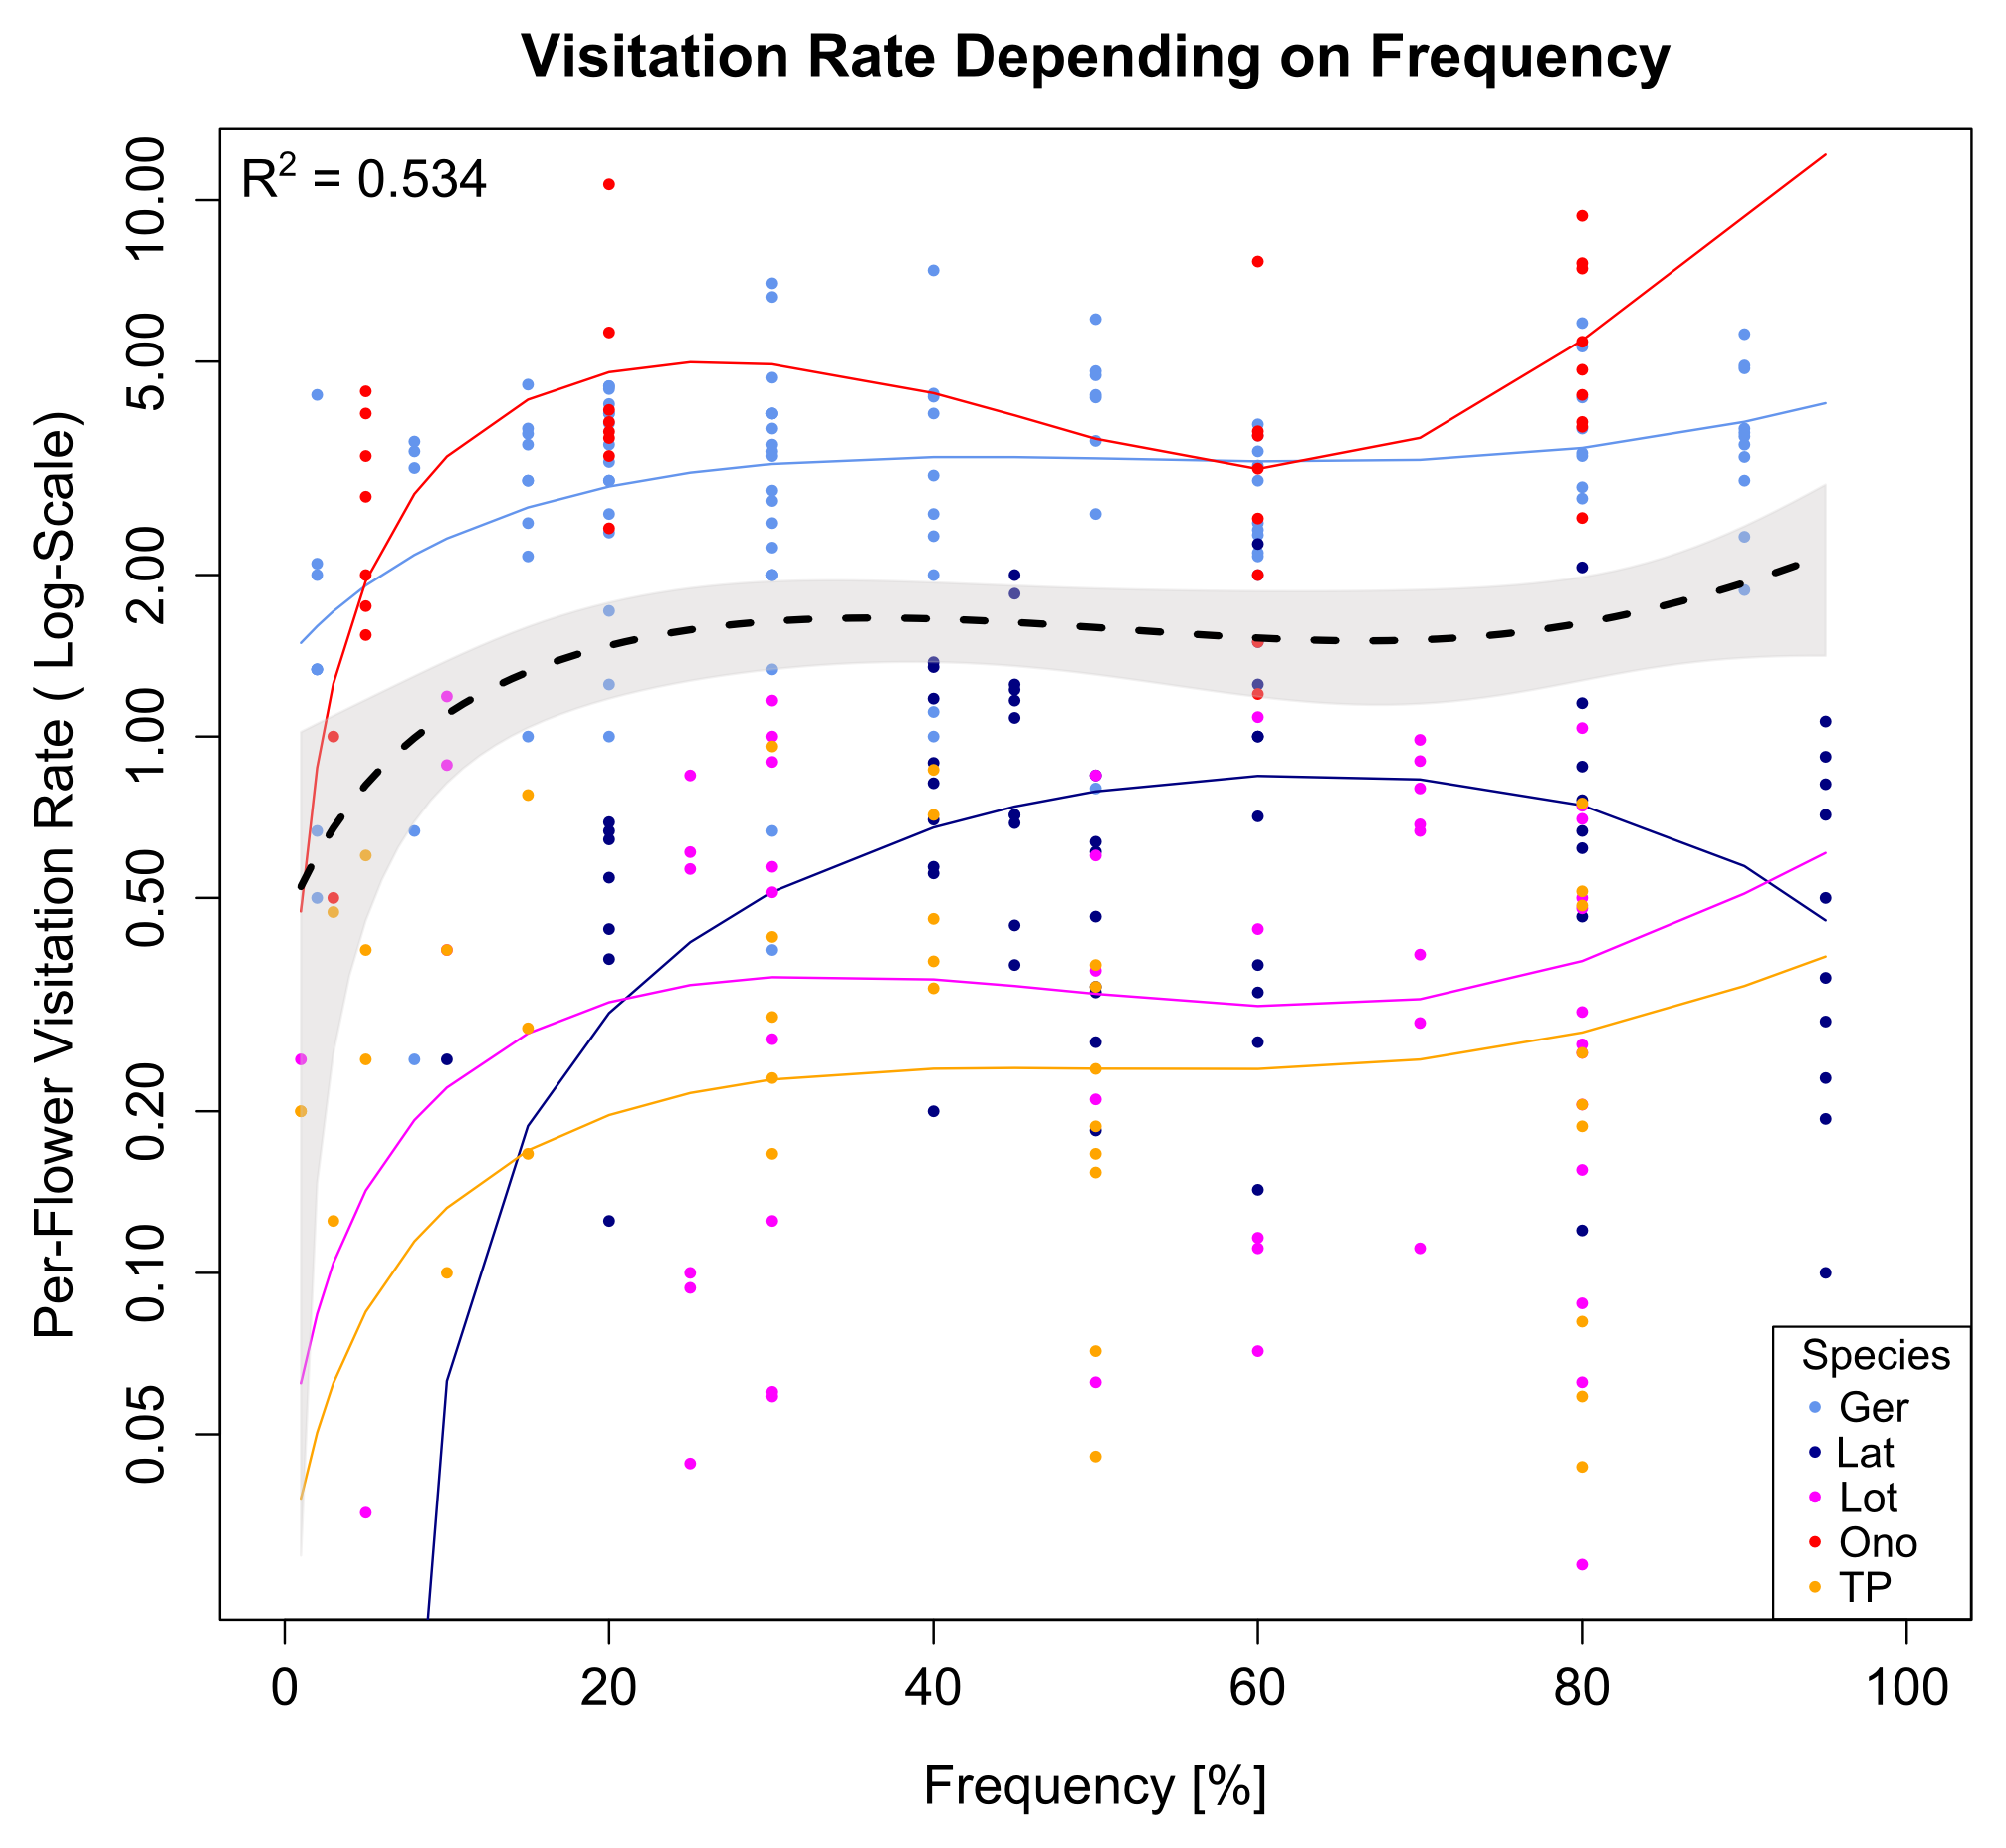
\includegraphics[width=14cm]{Images/LME}
 \caption{Per-flower visitation rates of the five focal species over different frequencies. Each point represents one observation of 15 minutes. The y-axis is plotted on a log scale due to the divergence in attractiveness of the focal species. The linear mixed effect model with Subplot nested in Plot as random factor show a sigmoidal frequency dependence for all species but \textit{Lathyrus pratensis}. Floral cover and species richness were dropped as explanatory variables in the model selection process. R$^{2}$ was calculated with the "r.squaredGLMM"-function of the MuMIn-Package \citep{MuMIn}}
 \label{fig:LME}
\end{figure}

%%%%%%%%%%%%%%%%%%%%%%%%%%

%\label{ch:appendix_ABM}

\section{Appendix}

%%%%%%results Jena%%%%%%%%%%%%%%%%%%%%

\begin{table}[!htbp] %VR species
	\centering
	\caption{Per-flower visitation rates (mean $\pm$ SD) for all focal flower species per 15 minute observation. \textit{Geranium pratense} and \textit{Onobrychis viciifolia} are significantly different from the other three species (pairwise t-test, \textit{p} $<$ 0.001) . Within the two groups, there is no significant difference between the species. }
	\begin{tabular}{l l l l l}
		\toprule
		\textbf {Short} & \textbf{Species} & \textbf{Family} &\textbf{Visitation Rate (Mean)} & \textbf{ $\pm$ SD} \\
		\midrule
		Ger  & \textit{Geranium pratense} & Geraniaceae & 3.05 & 1.5 \\ %109
		Lat  & \textit{Lathyrus pratensis} & Fabaceae & 0.57 & 0.53 \\ %83
		Lot  & \textit{Lotus corniculatus} & Fabaceae & 0.30 & 0.36 \\  % 77
		Ono  & \textit{Onobrychis viciifolia} & Fabaceae & 3.60  &  2.5 \\ % 37
		TP   & \textit{Trifolium pratense} & Fabaceae & 0.16 & 0.23 \\ % 79
		\bottomrule
	\end{tabular}%
	\label{tab:VR_spec}
\end{table}%

\begin{table} [!htbp] %results lme
	\centering
	\caption{Results of the linear mixed effect model with per-flower visitation rate as explanatory variable. Floral cover and species richness were not relevant predictors for the model and therefore removed in the model selection process (denDF = 191, R$^{2}$ = 0.53, n = 385)}
	\begin{tabular} { l l c c c}
		\toprule
		\textbf{Response Variable} & \textbf{Explanatory Variables} & \textbf{Df} & \textbf{F-value} & \textbf{\textit{P}} \\
		\midrule
		Per-flower visitation rate   & Species & $4$ & $130.9$ & $<0.0001$\\
		& Frequency 			&  $1$ & $49.3$ & $<0.0001$ \\
		& Frequency$^{2}$ 		&  $1$ & $13.2$ & $0.0026$ \\
		& Frequency$^{3}$ 		&  $1$ & $ 5.8$ &  $0.8145$ \\
		& Frequency x Species &  $4$ & $ 5.2$ &  $0.0005$ \\
		& Frequency$^{2}$ x Species & $4$ & $3.4$ & $0.0097$\\
		& Frequency$^{3}$ x Species & $4$ & $3.4$ & $0.0101$\\
		\bottomrule
	\end{tabular}
	\label{tab:anova}
\end{table}

\begin{figure} [!h] %LME
	\centering
	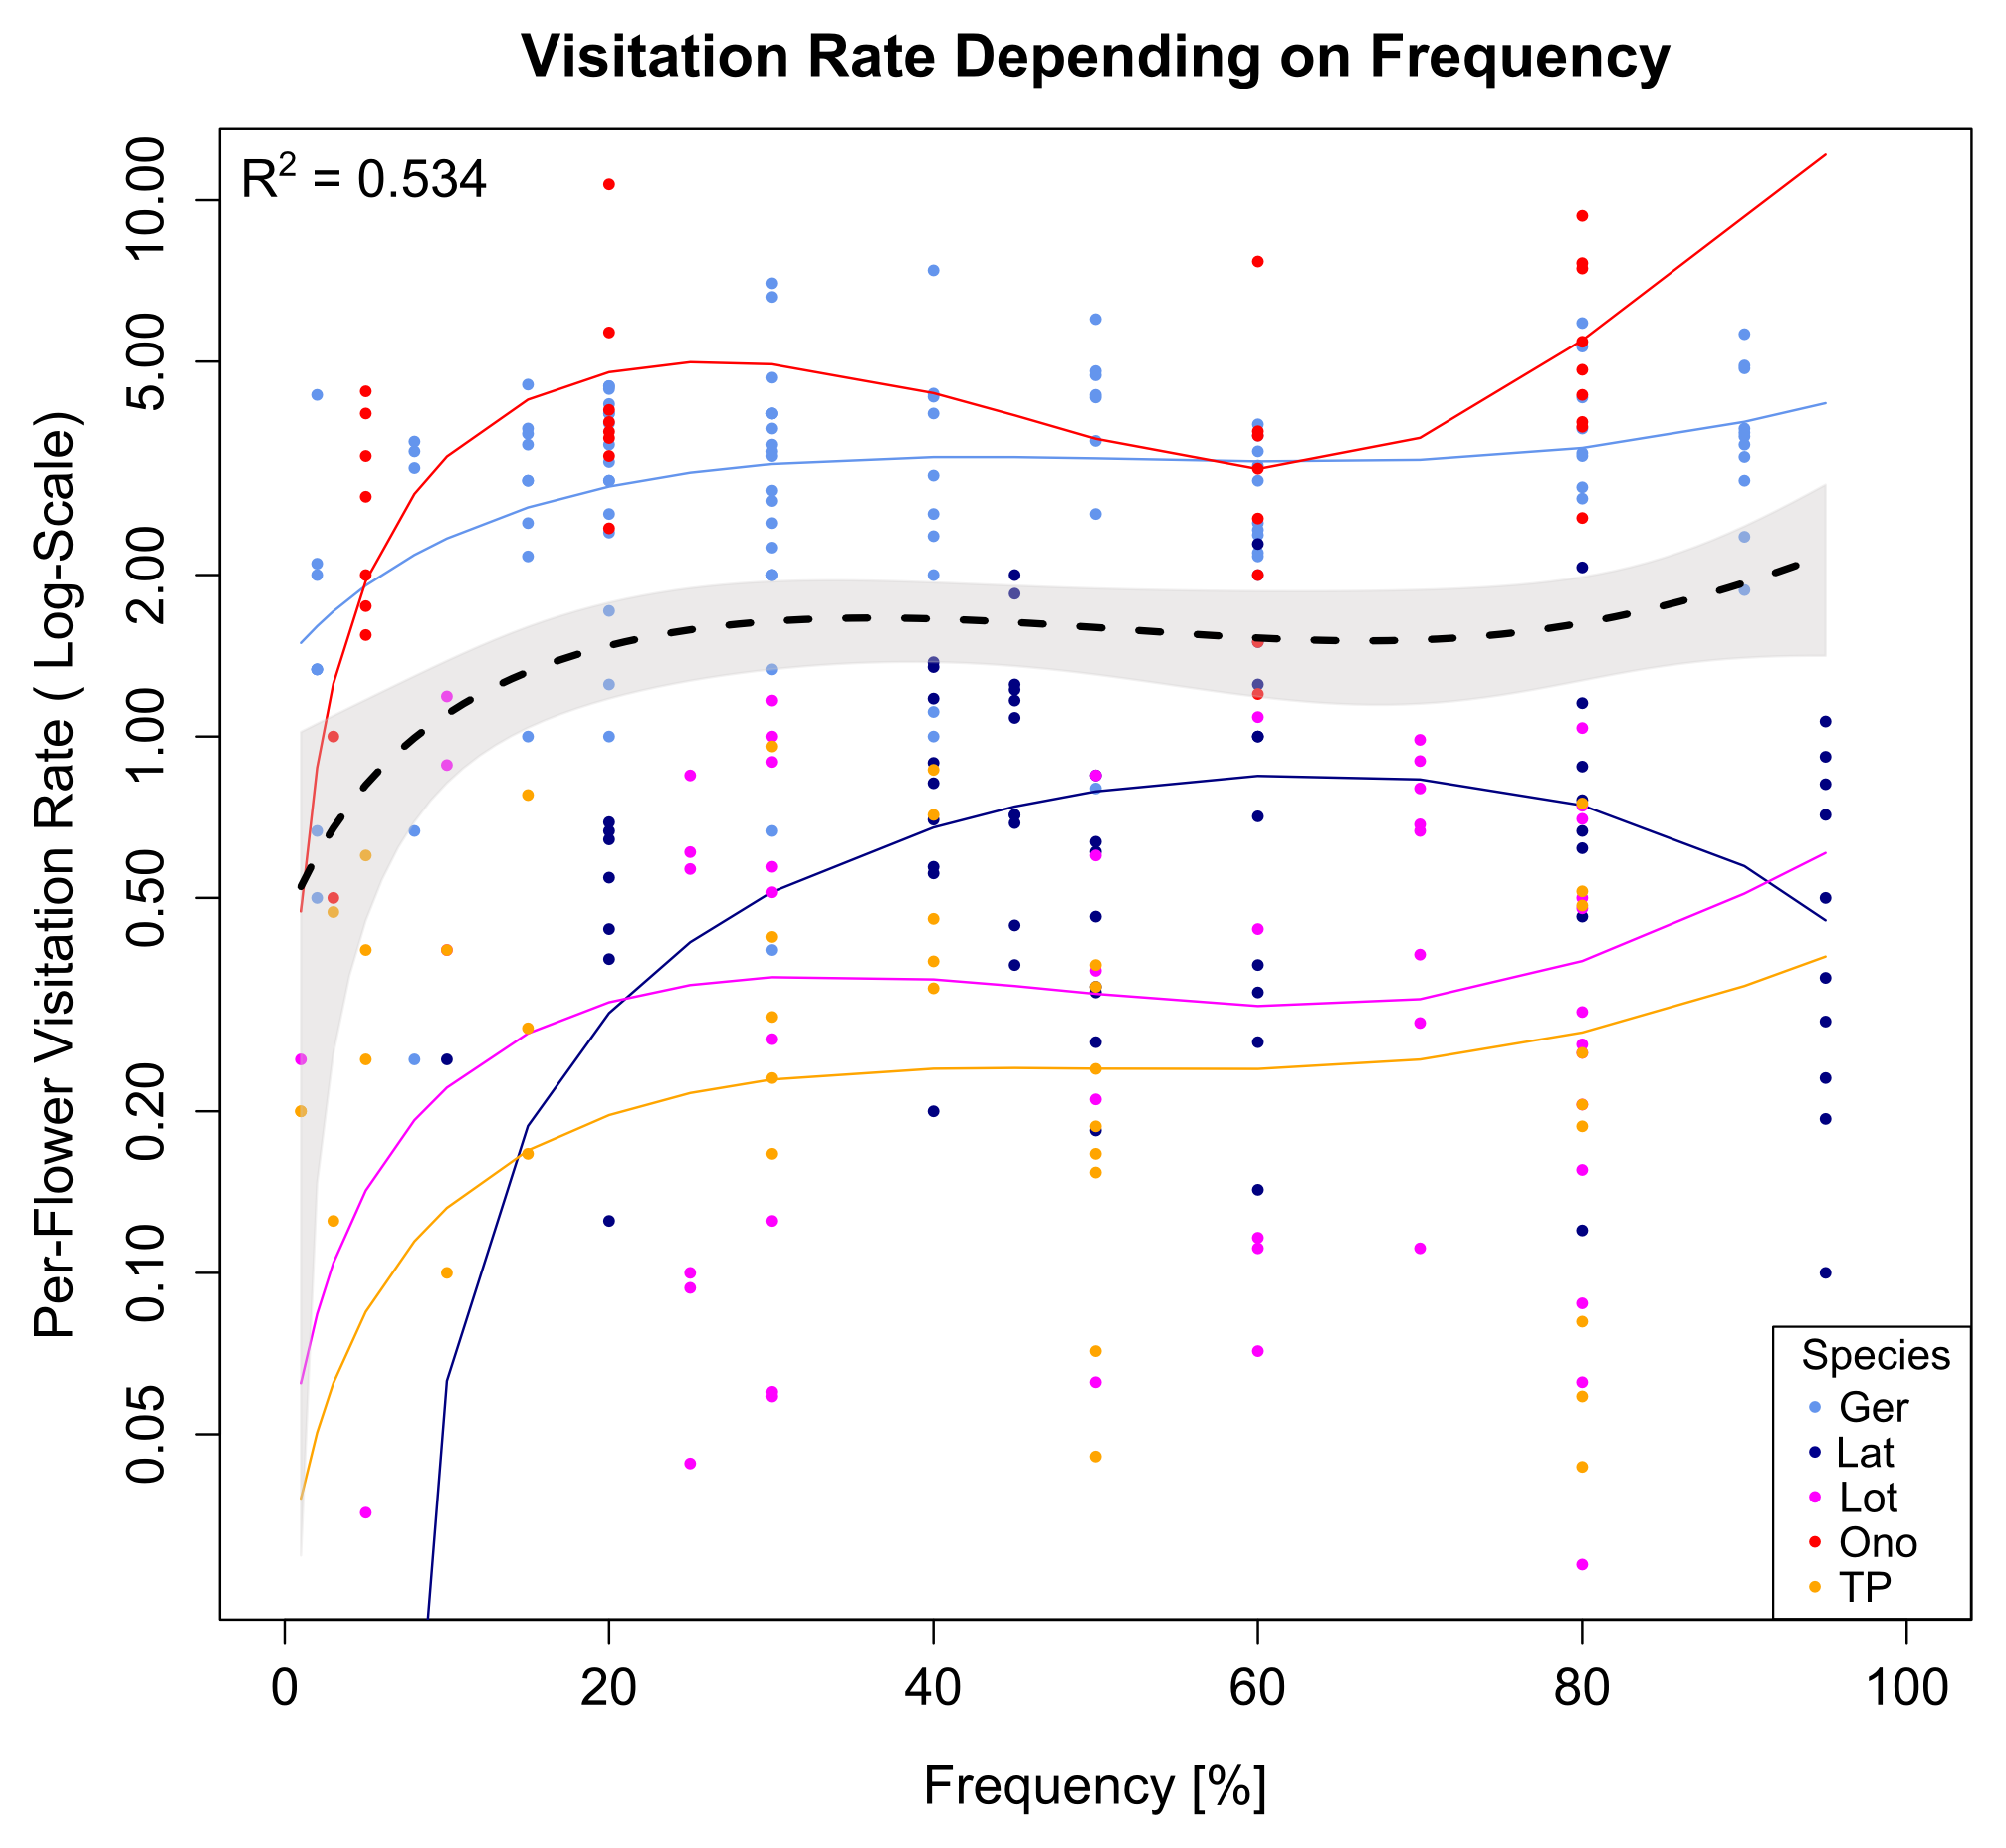
\includegraphics[width=14cm]{Images/LME}
	\caption{Per-flower visitation rates of the five focal species over different frequencies. Each point represents one observation of 15 minutes. The y-axis is plotted on a log scale due to the divergence in attractiveness of the focal species. The linear mixed effect model with Subplot nested in Plot as random factor show a sigmoidal frequency dependence for all species but \textit{Lathyrus pratensis}. Floral cover and species richness were dropped as explanatory variables in the model selection process. R$^{2}$ was calculated with the "r.squaredGLMM"-function of the MuMIn-Package \citep{MuMIn}}
	\label{fig:LME}
\end{figure}

%%%%%%%methods model%%%%%%%%%%%%%%%%%%%
\clearpage

\begin{figure} [!h] % screenshots
	\centering
	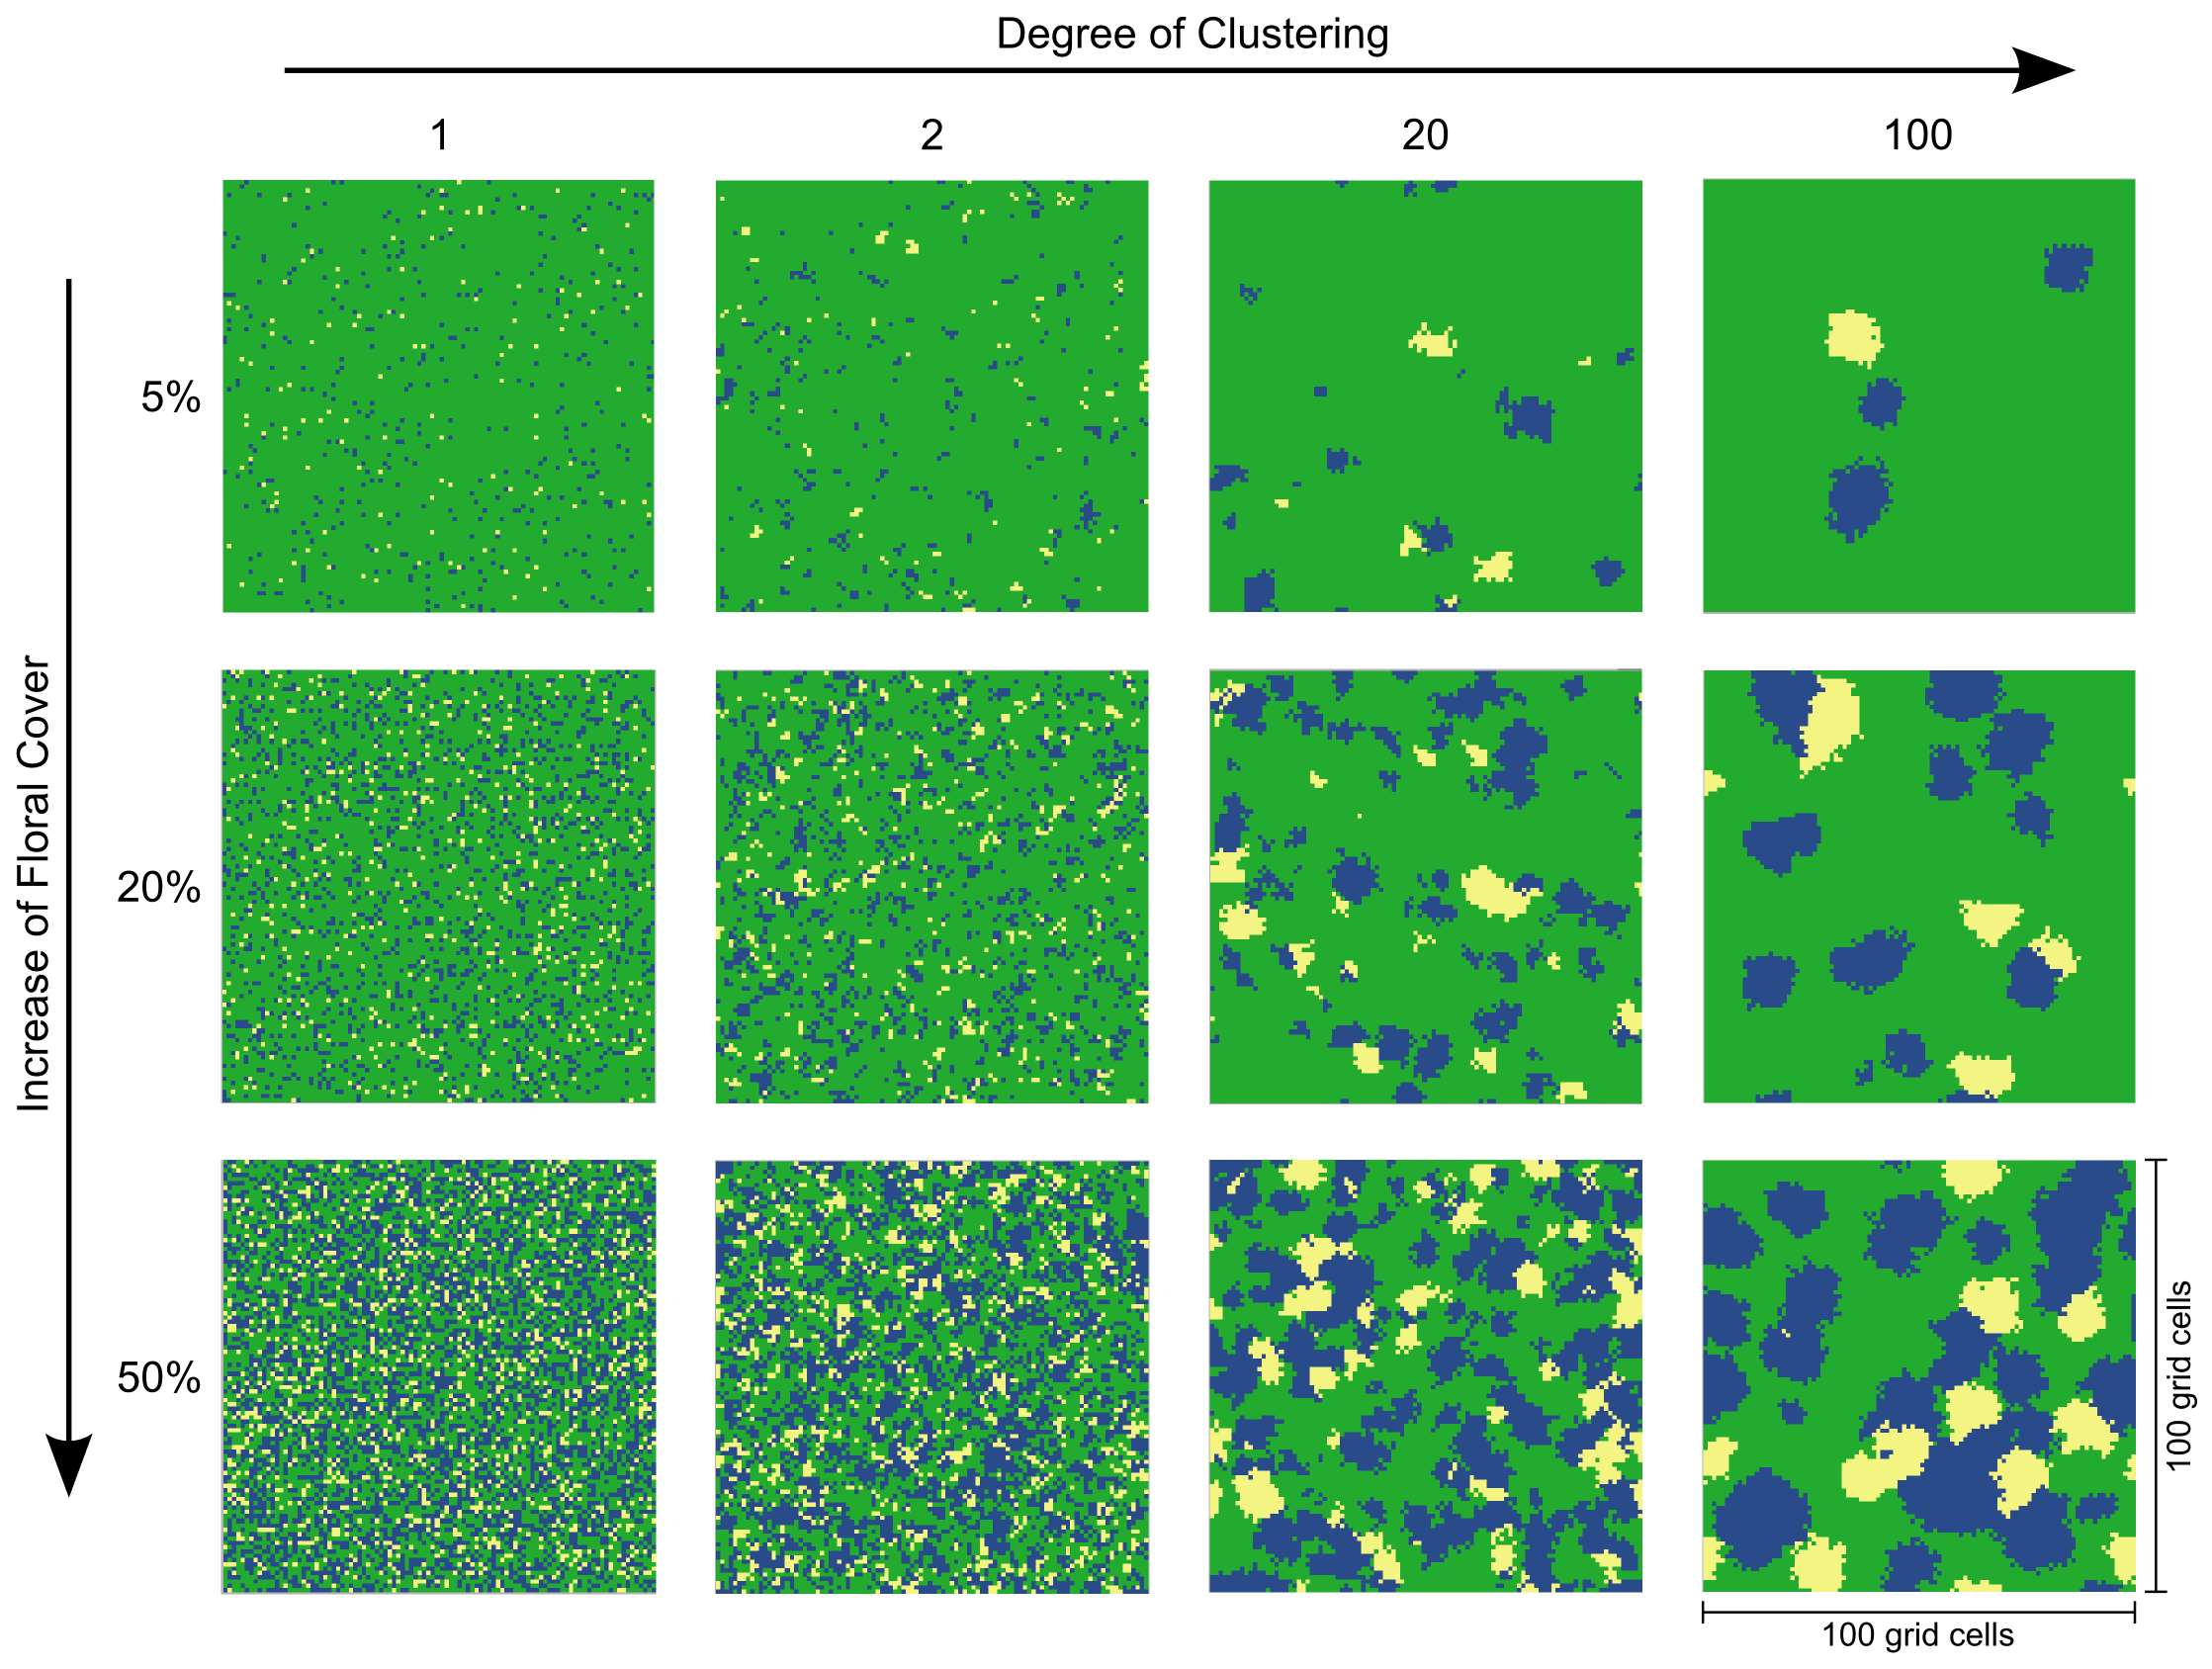
\includegraphics[width=15cm]{Images/cluster}
	\caption{ Exemplary model environment setups with increasing floral cover and degree of clustering. The cover expresses the percentage of patches containing a flower ($\Sigma_{patches}$ = 10 000). The cluster number equals the average amount of flowers per cluster. Flowers are randomly assigned to the clusters to achieve a more natural, uneven distribution. }
	\label{fig:cluster}
\end{figure}

\begin{figure} [!h] %flowchart
	\centering
	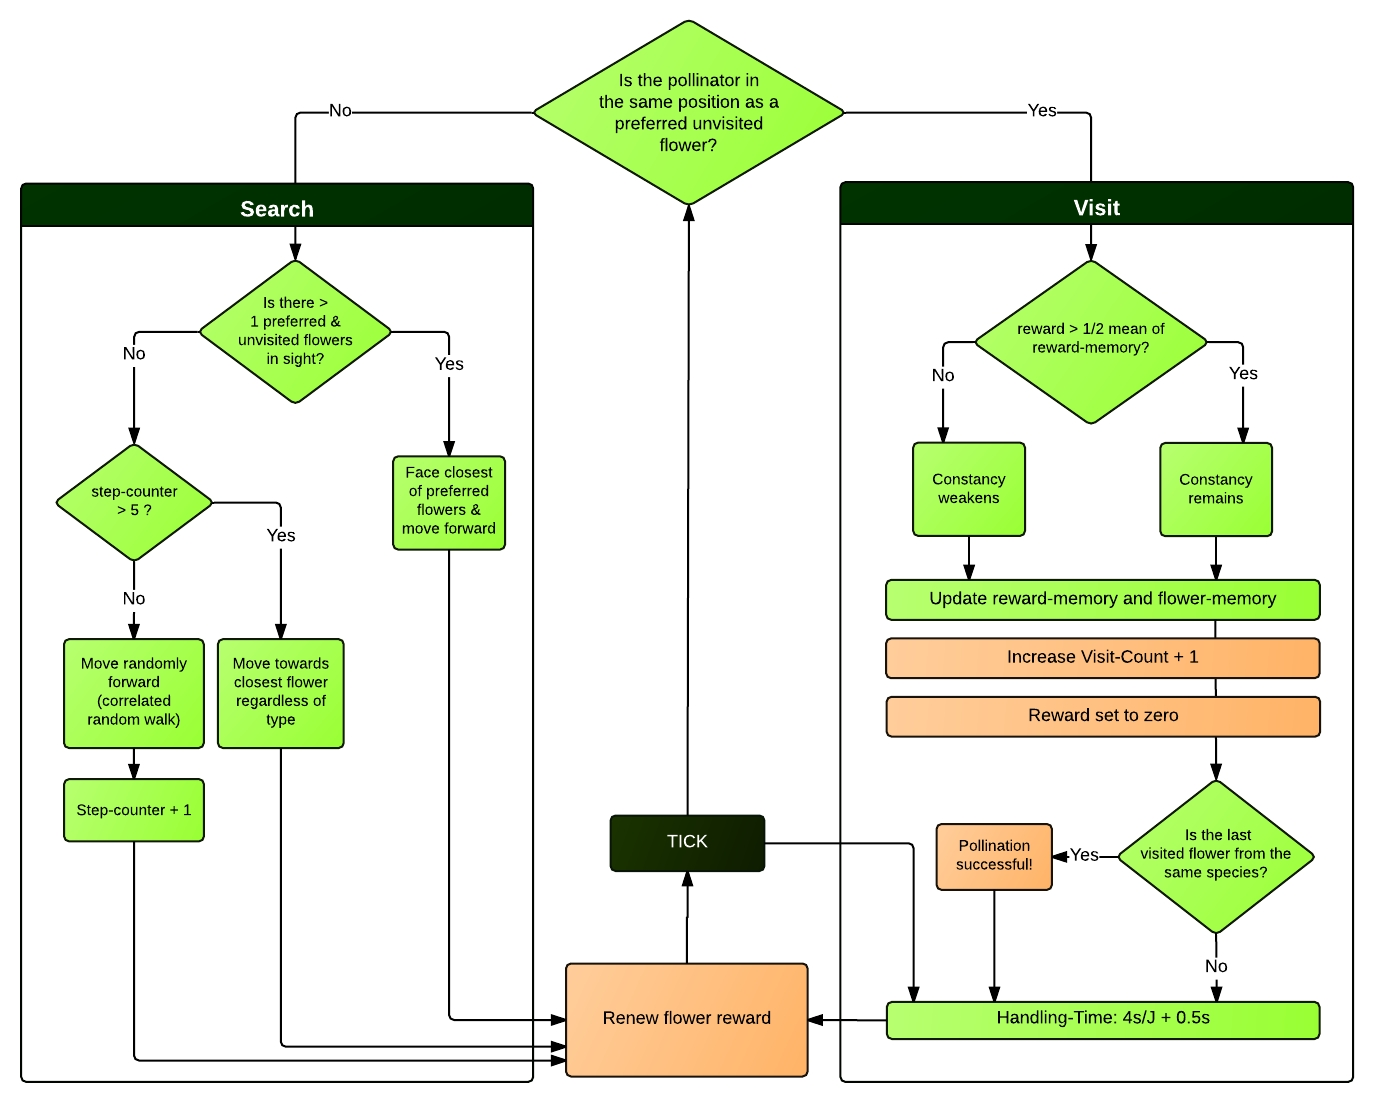
\includegraphics[width=15cm]{Images/flowchart-model}
	\caption{Flowchart describing the behavior rules for the bee-agents within the agent-based model. Every bee-agent can either search for a preferred flower or visit one. While searching, a bee-agent can remember the location of the last four visited flowers to avoid double-encountering. If there is no flower in sight after 5 seconds of correlated random walk (CRW), the probability that it will encounter the next available flower despite its type increases by 10\% per additional time step. When a bee-agent visits a flower it takes all reward within a reward-dependent handling time and compares the amount with its memory. If the reward is low, the agent is more likely to visit the other flower type next time. The maximum of visits within a successful pollination is possible is determined by the pollen carryover rate.}
	\label{fig:flowchart}
\end{figure}

\begin{table} [!htbp] %parameter values
	\centering
	\caption{Parameter values used for the main and sensitivity analysis. Only general parameters were changed in the main analysis, whereas the sensitivity analysis also directly influences the behavior of the bee-agents. Within the main analysis, each combination was run 20 times for 1000 ticks, that makes a total of 110,400 runs in the main analysis and 16,560 runs for each parameter of the sensitivity analysis. }
	\begin{tabular} {l l l}
		\toprule
		\textbf{Parameter} & \textbf{Description}  & \textbf{Values}\\
		\midrule
		\addlinespace[0.2cm]
		\multicolumn{ 3} {l} {\textsc{Main analysis}} \\ 
		\addlinespace[0.2cm]
		Frequency & Proportion of species A on all flowers  & 0-100\% (5\%-steps)\\
		Flower cover & Proportion of patches being flowers  & 5, 10, 20, 50 \%\\
		Degree of clustering & Average number of flowers per cluster   &  1, 2, 5, 10, 20, 50, 75, 100\\
		Pollen-carryover rate & Number of visits within a successful pollination is possible & 1, 2, 4, 6, 8, 16\\
		
		\addlinespace[0.2cm]
		\multicolumn{ 3 } {l} {\textsc{Sensitivity analysis}} \\ 
		\addlinespace[0.2cm]
		Reward function & Increase of reward per flower and second & 0, 0.00004, 0.001, 0.1 J/sec \\
		Vision distance & Max. range of patches within a bee-agent can detect flowers & 1, 6, 20, 50 patches\\
		Search time & \begin{tabular}{@{}l@{}} Number of seconds a bee-agent searches before\\ probability of switching flowers increases \end{tabular}   & 1, 5, 20, 50 sec \\
		Pollinator density & Number of bee-agents on the meadow & 5, 10, 20, 50 bees\\
		
		\bottomrule
	\end{tabular}
	\label{tab:simulation_run}
\end{table}

%%%%%%%results ABM %%%%%%%%%%%%%%%%%%%%
\clearpage

\begin{figure} [!h] %results:SUM
	\centering
	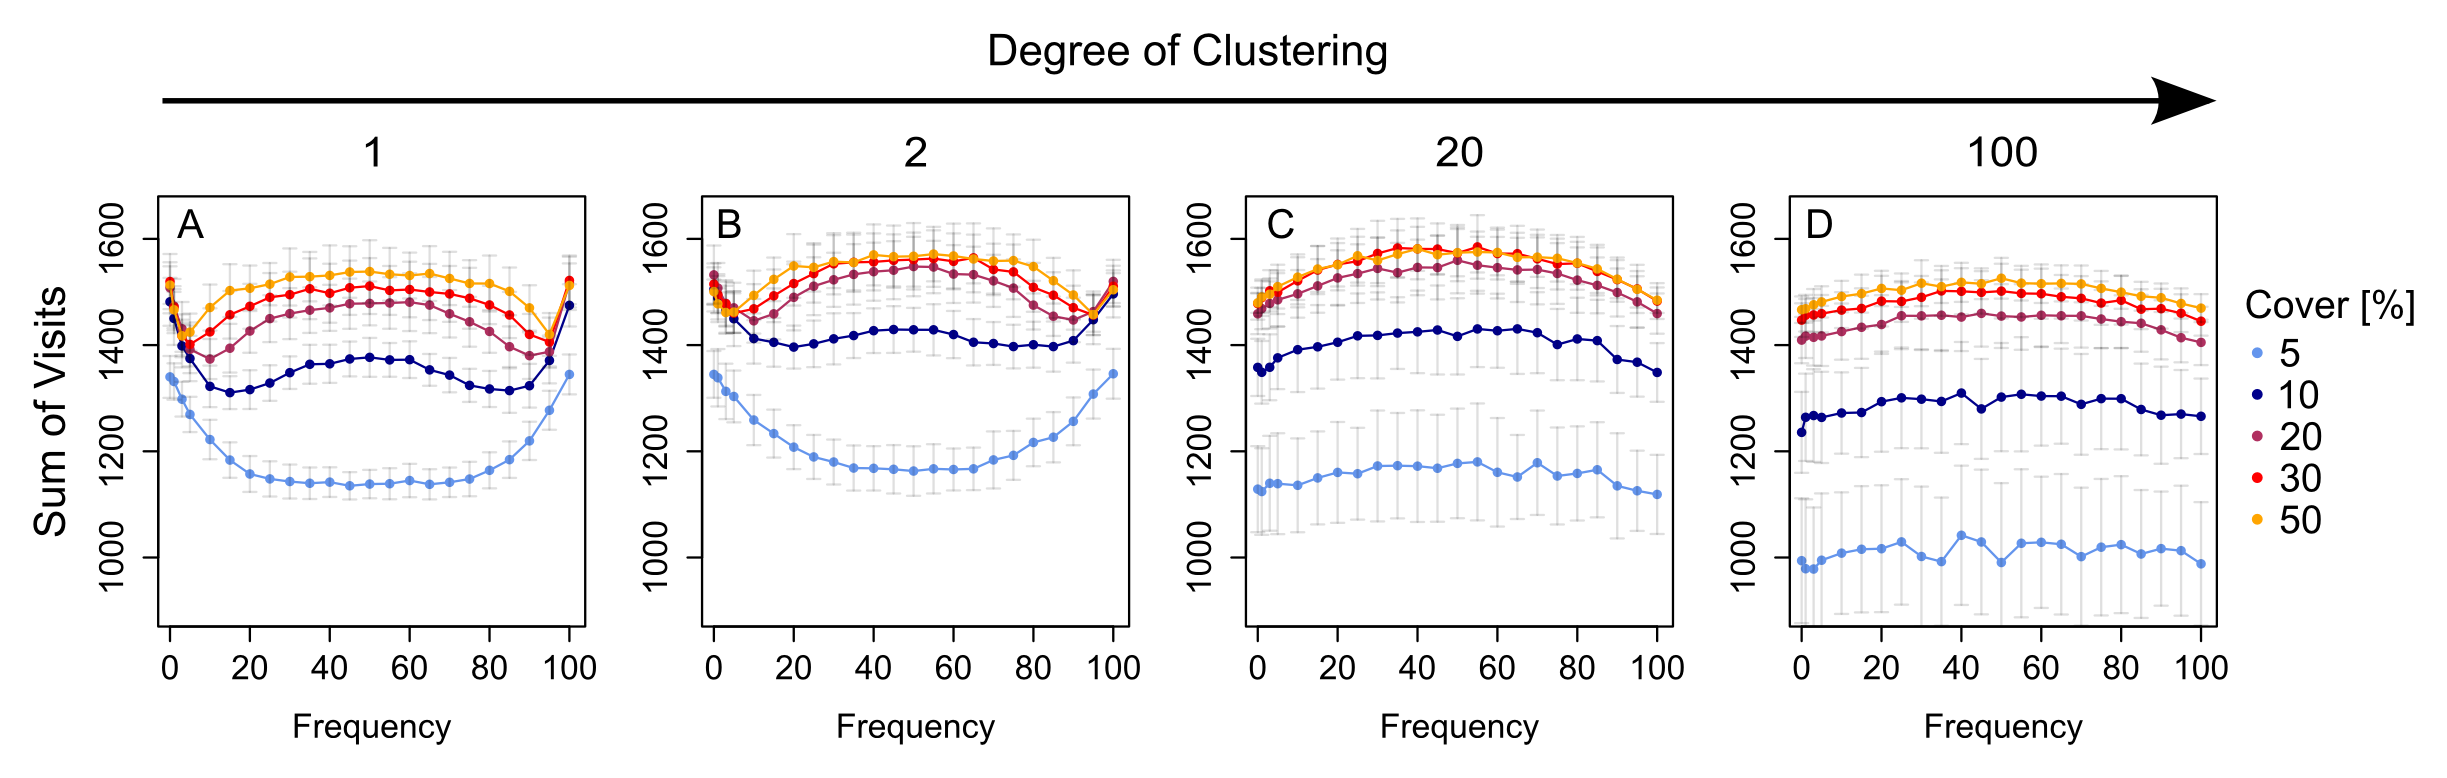
\includegraphics[width=17cm]{Images/SUM}
	\caption{Summed visits to both species show a frequency dependence for low cluster values. Depending on the floral cover it is quadratic or a fourth-degree polynomial relationship. Maximum of visits (maximal efficiency) is achieved for very unequal or very equal frequencies. If one species is rare, the sum of visits drop because some bee-agents forage inefficiently on the rare species, having long flight and searching times. Clustering reduces the frequency dependence but also decreases the absolute number of visits and increases the variance (grey error bars).}
	\label{fig:SUM}
\end{figure}

\begin{figure} [!ht] %results:PFV
	\centering
	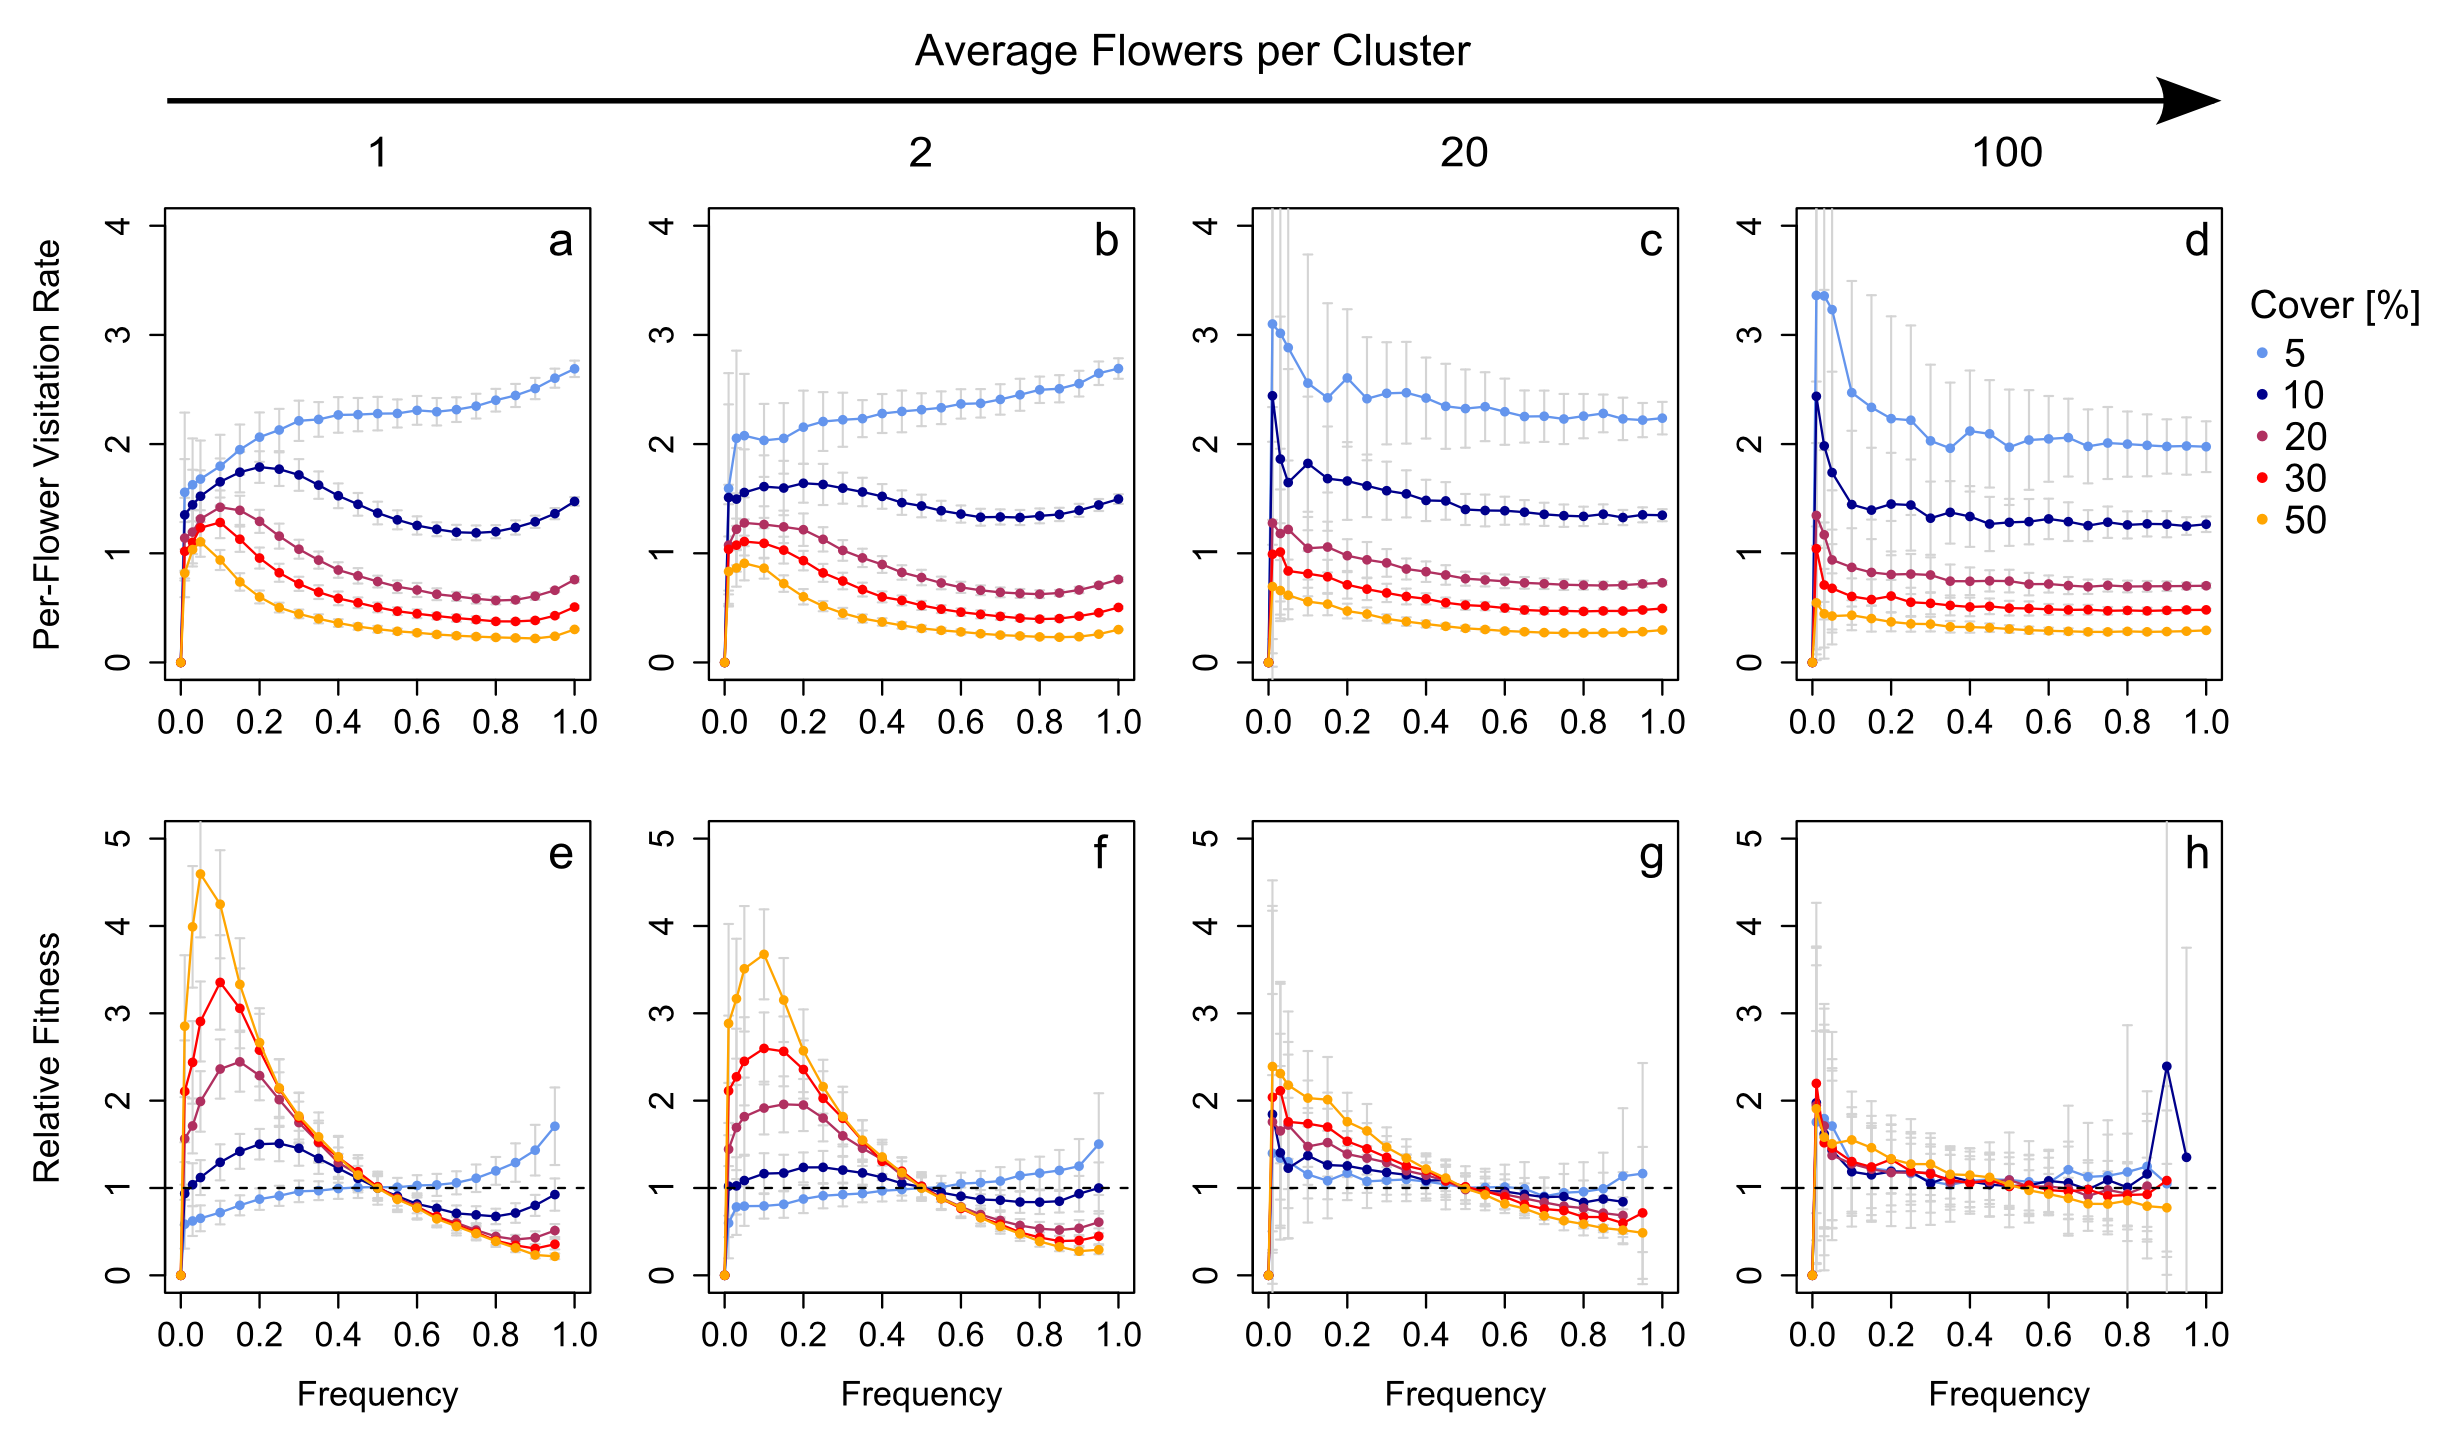
\includegraphics[width=17cm]{Images/PFV}
	\caption{The main analysis of the agent-based model confirm the findings of the linear mixed effect model of the field data: The per-flower visitation rate shows a clear frequency dependence with a cubic relationship. Visitation rates increase within the first 10-20\% of frequency towards a maximum. For intermediate frequencies is the increase of flowers not proportional with additional visits. The per-flower visitation rate only increases again towards exclusiveness of the species. The effect is stronger for higher floral cover (2a-d). Increase in clustering reduces the frequency dependence (1d,2d).}
	\label{fig:PFV}
\end{figure}

\begin{figure} [!ht] %results:POC
	\centering
	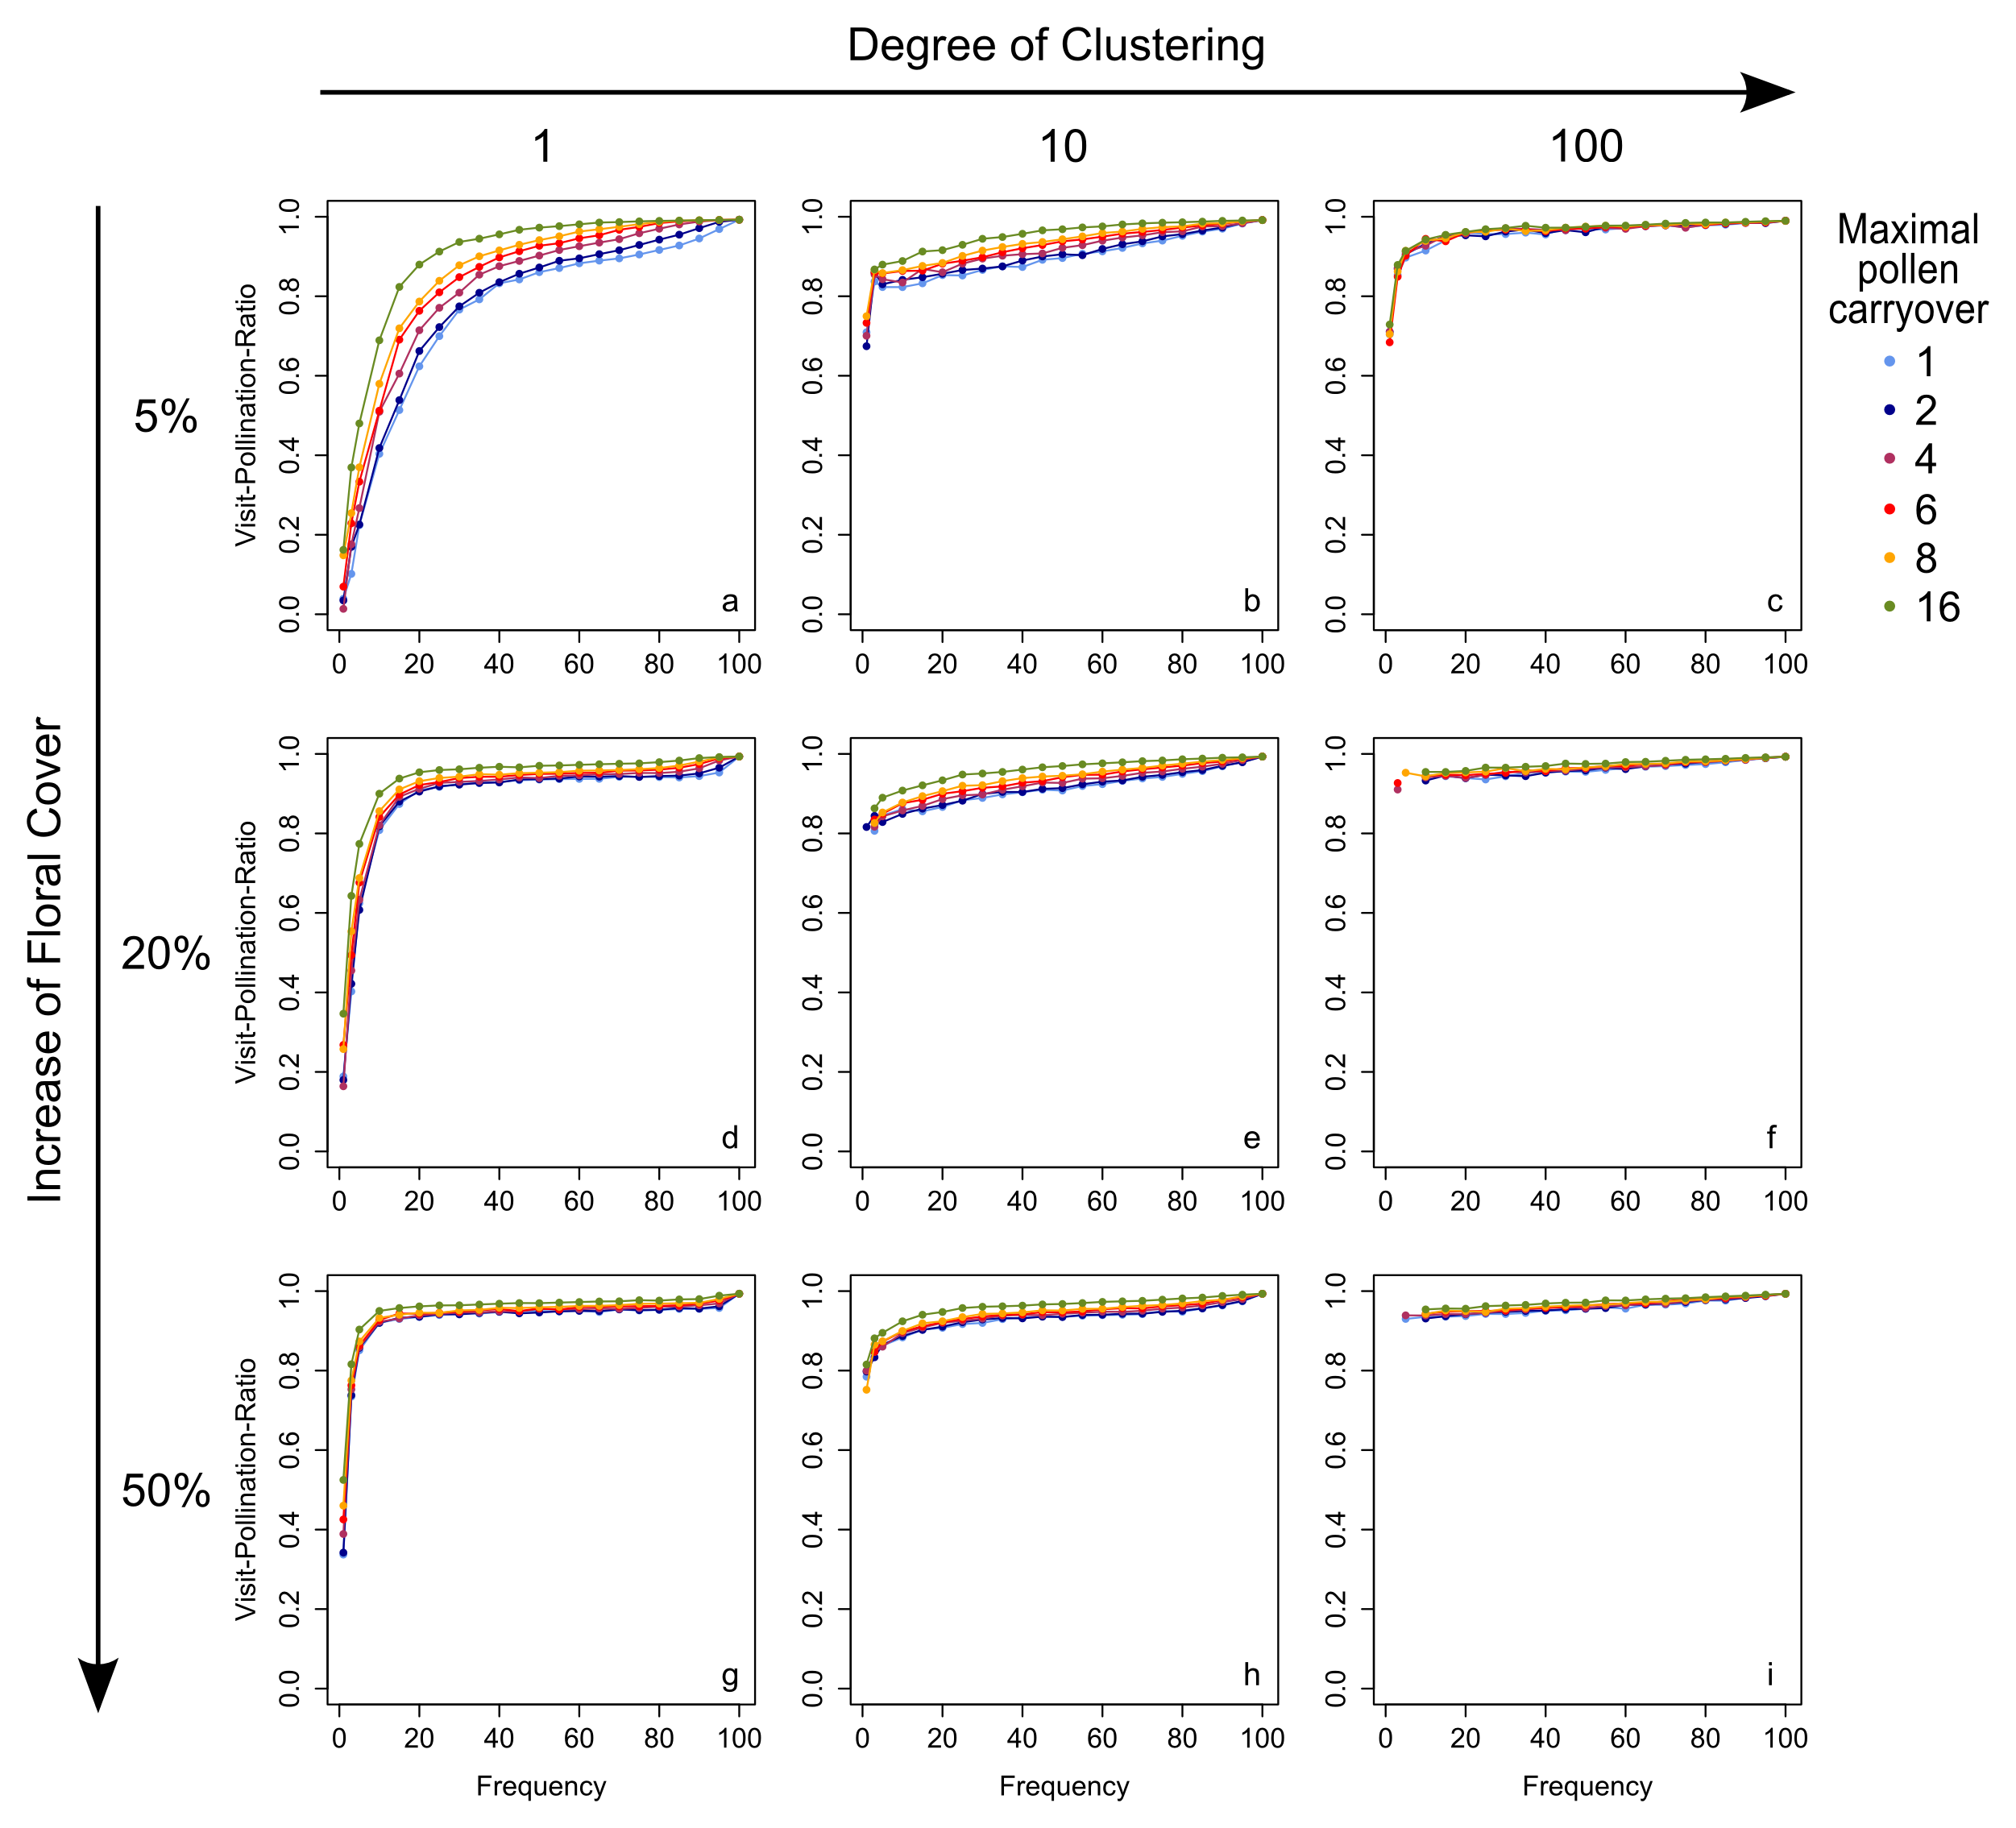
\includegraphics[width=17cm]{Images/POC}
	\caption{The pollen-carryover rate defines the maximum number of visits within a successful pollination is possible. With a pollen-carryover rate of one, the pollen can only be carried to the next flower. Therefore, the ratio of successful pollinations per visit can be seen as indicator for flower constancy \citep{montgomery2009pollen}. A high pollen-carryover rate is only important for a low cover and no-cluster environment. With increasing cover and cluster, the ratio becomes steeper for low frequencies which stands for more qualitative visits.}
	\label{fig:POC}
\end{figure}

\newpage

\label{ch:supplementary_material}

\section*{Supplementary Material}
\beginsupplement

\begin{table}[!htbp]
	\centering
	\caption{List of the focal species observed in the natural condition experiment within the area of the Jena Experiment. Species had to flower in at least five plots with different frequency values.}
	\begin{tabular}{llllll}
		\toprule
		\textbf{Short} & \textbf{Name} & \textbf{German Name} & \textbf{Order} & \textbf{Family} & \textbf{Color} \\
		\midrule
		Ger   & \textit{Geranium pratense} & Wiesen-Storchschnabel & Geraniales & Geraniaceae & Purple \\
		Lat   & \textit{Lathyrus pratensis} & Wiesen-Platterbse & Fabales & Fabaceae & Yellow \\
		Lot   & \textit{Lathyrus pratensis} & Gewöhnliche Hornklee & Fabales & Fabaceae & Yellow \\
		Ono   & \textit{Onobrychis viciifolia} & Saat-Esparsette & Fabales & Fabaceae & pink+white \\
		TP    & \textit{Trifolium pratense} & Wiesen-Klee & Fabales & Fabaceae & Purple \\
		\bottomrule
	\end{tabular}%
	\label{tab:Species}
\end{table}%

%%%%%%%%%%%%%%%%%%%%%%%%%%

\begin{figure} [H] %plot-design
\centering
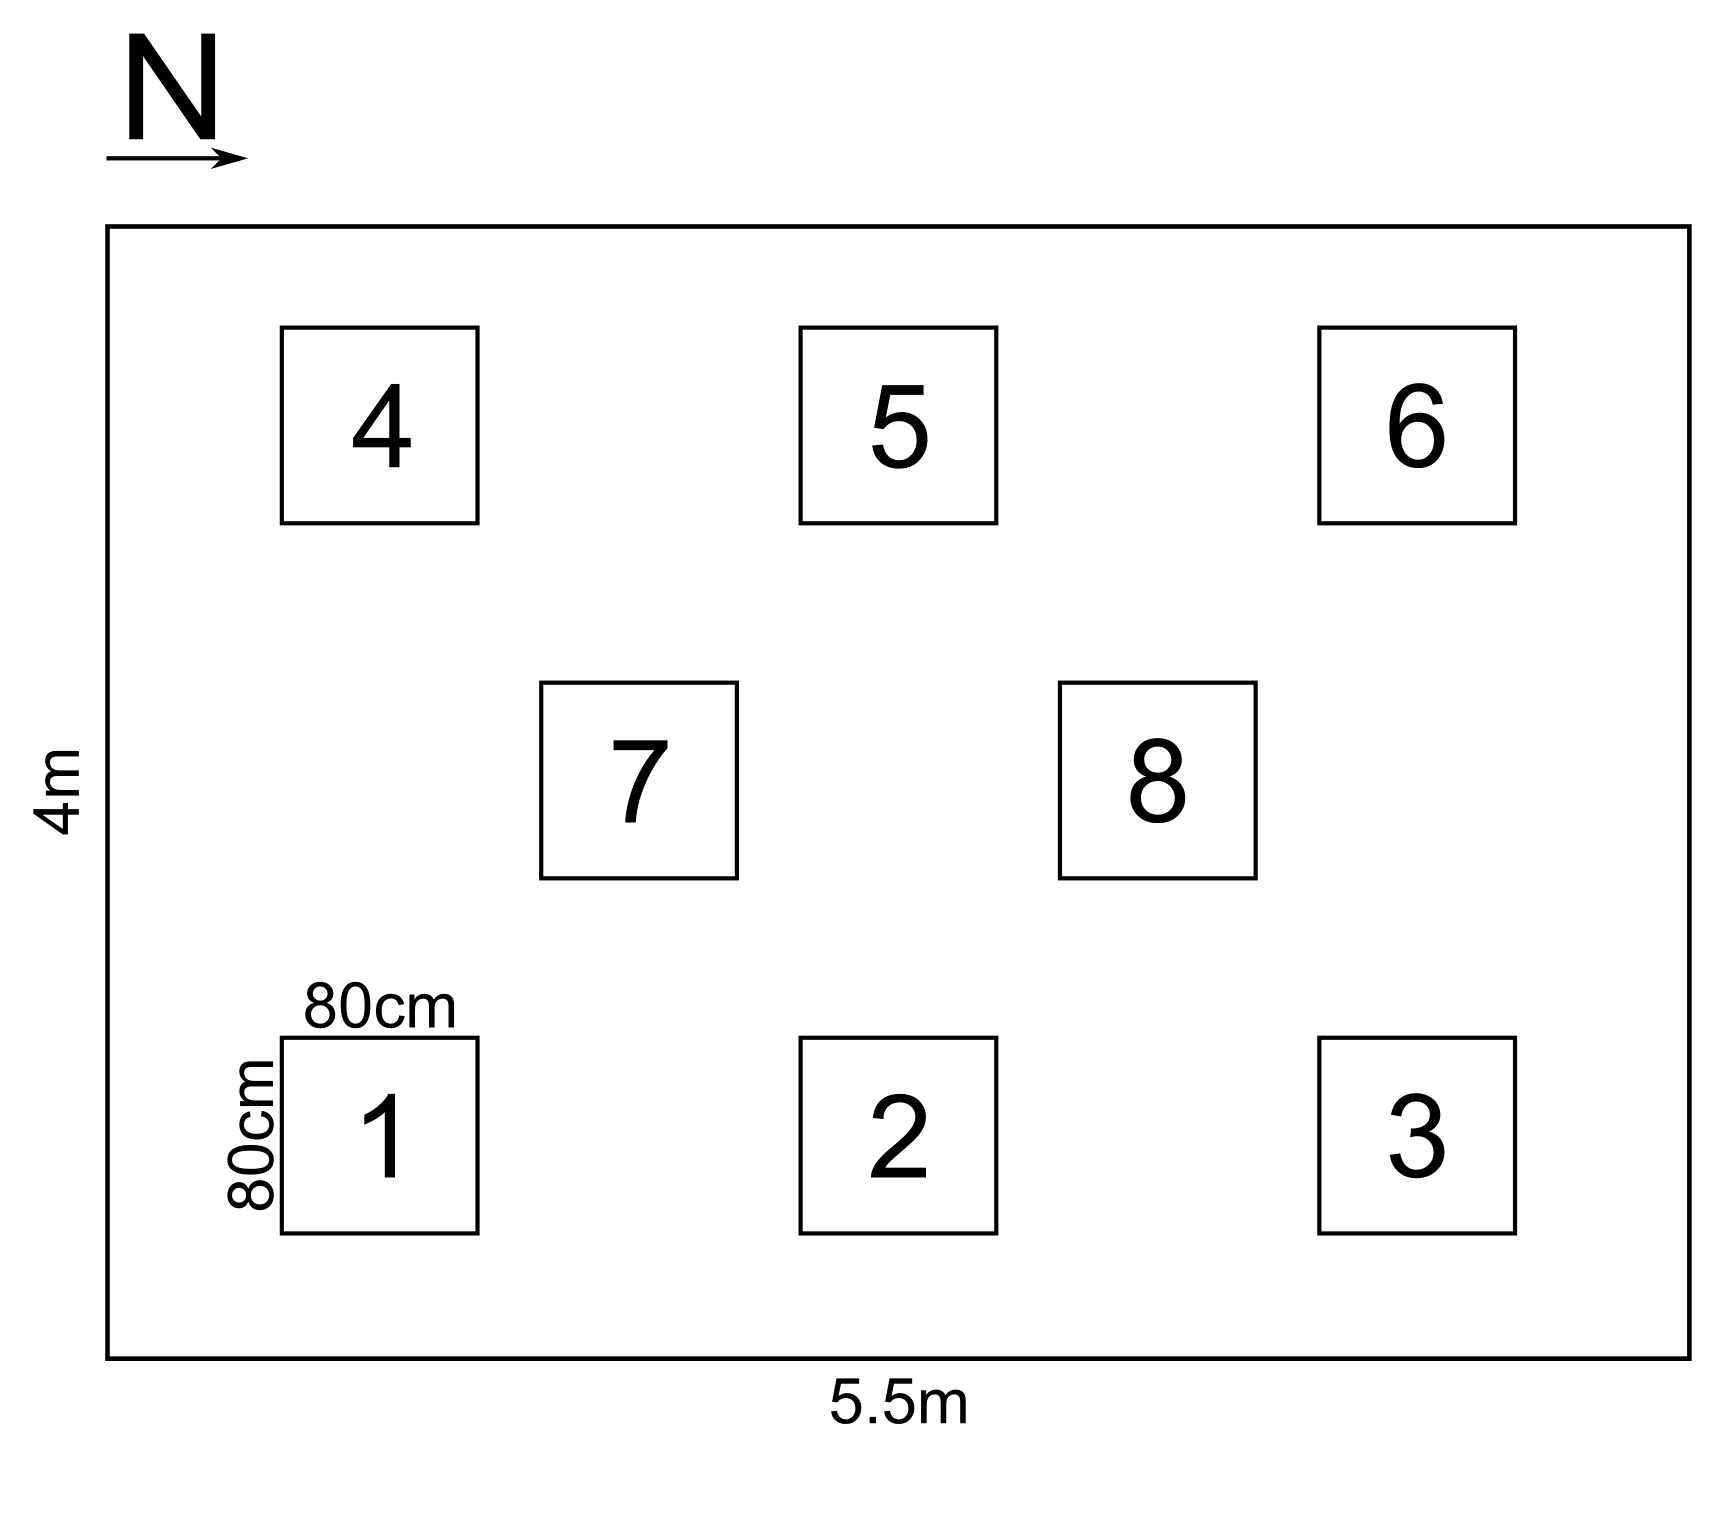
\includegraphics[width=9cm]{Images/plot-design}
 \caption{The distribution of subplots within the old invasion plots.}
 \label{fig:plot-design}
\end{figure}


%%%%%%%%%%%%%%%%%%%%%%%%%%
\newpage

\begin{figure} [H] %pairs-plot
\centering
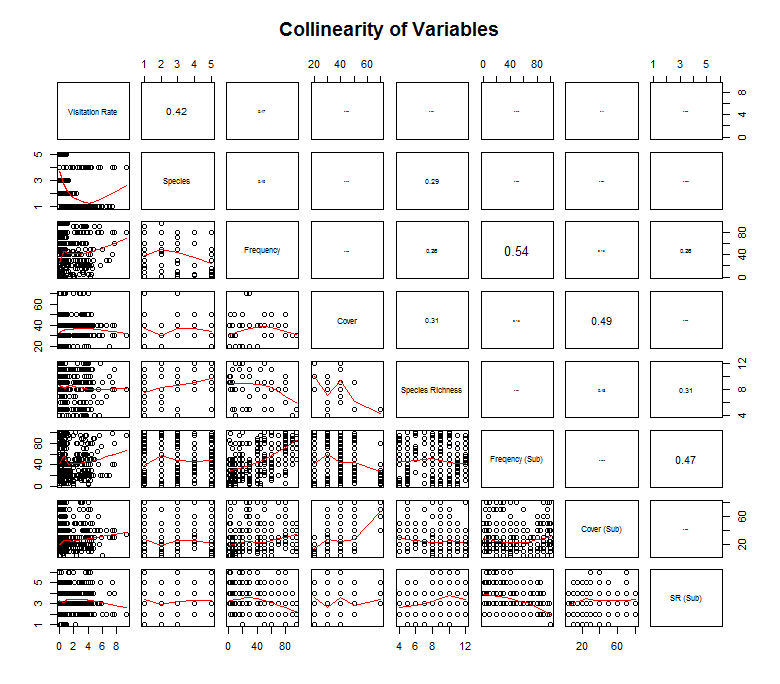
\includegraphics[width=16cm]{Images/pairs-plot}
 \caption{Pairwise correlation of Visitation rate (response variable), species, frequency, floral cover and species richness on plot and subplot-level. The upper panels contain Pearson correlation coefficients with its size proportional to its value. Parameters correlate on the plot and subplot level but show no strong correlation not among each other.}
 \label{fig:pairs-plot}
\end{figure}

%%%%%%%%%%%%%%%%%%%%%%%%%%

\begin{table}[!htbp] 
  \centering
  \caption{Variance inflation factors (VIF) for the full set of variables. Values are calculated by the "corvif"-function from R-package AED. All values are well below three indicating no collinearity (see \citet{zuur2007analysing}).}
  %cite for AED/Zuur
    \begin{tabular}{ll}
    \toprule
    \textbf{Variable} & \textbf{GVIF}\\
    \midrule
    Visitation Rate  	&  1.26\\
    Species 			 &  1.36\\
    Frequency 	  	    &  1.63\\
    Floral Cover   		 &  1.46\\
    Species Richness     &  1.45\\
    Frequency (Subplot) 	    &  1.84\\
    Floral Cover (Subplot)		  &  1.37\\
    Species Richness (Subplot)    &  1.48\\
    \bottomrule
    \end{tabular}%
\label{tab:VIF}
\end{table}%

%%%%%%%%%%%%%%%%%%%%%%%%%%
\clearpage

\begin{figure} [H] %residuals
\centering
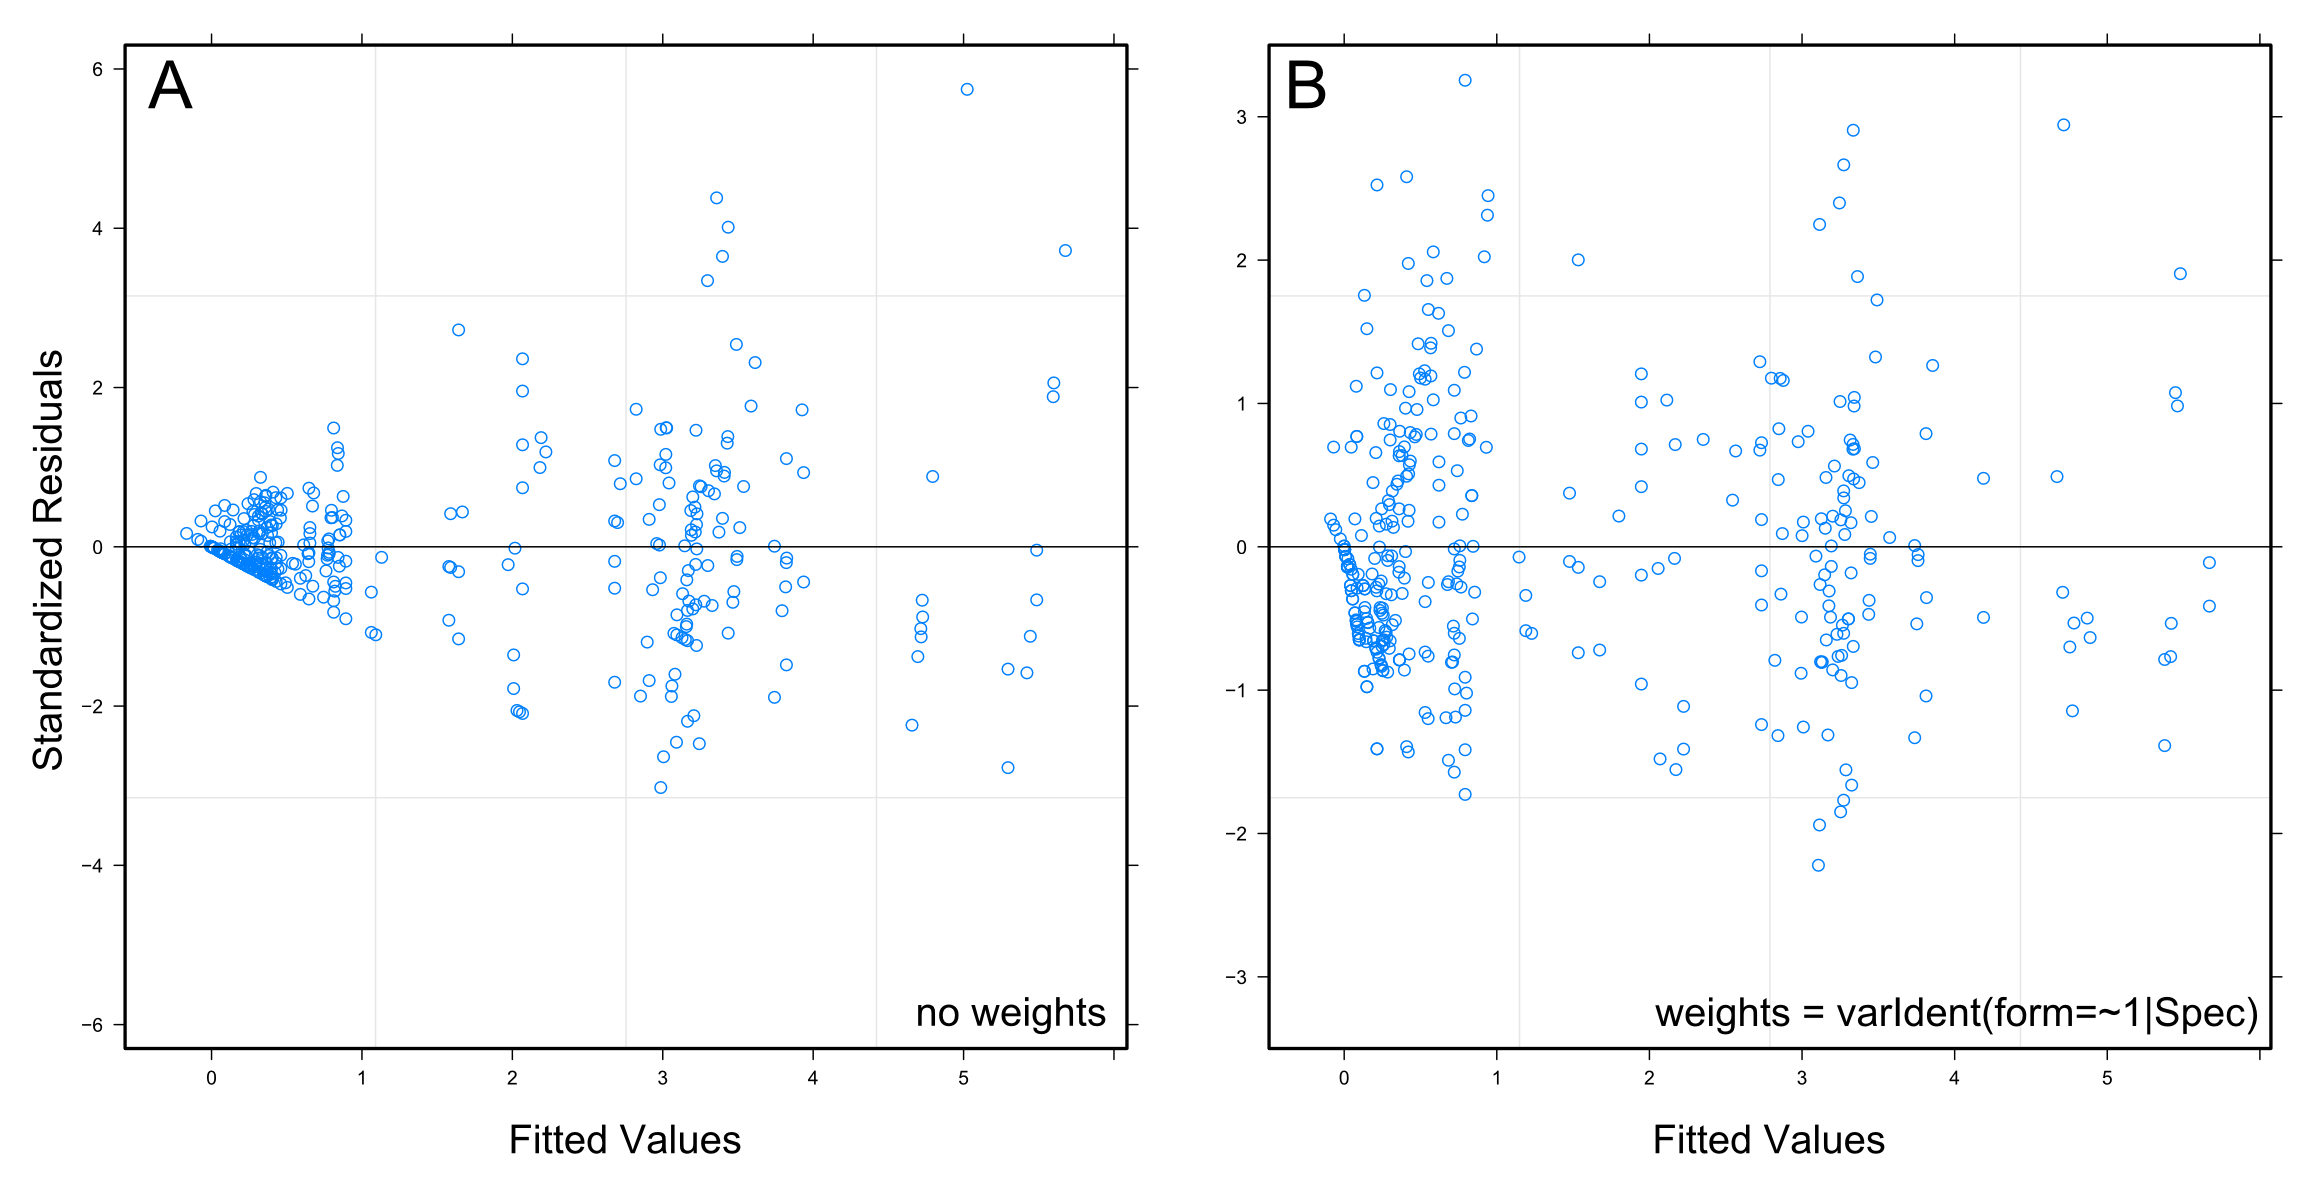
\includegraphics[width=15cm]{Images/residuals}
 \caption{Standardized residuals plotted against fitted values for the final mixed effect model with and without applied weighting. A) Without weighting, the residuals show strong pattern of heteroscedasticy. B) The weighting allows different variance per species. The final model is significantly better with weighting (\textit{L}=393.32, df= 4, \textit{P} $<$ 0.0001)}
 \label{fig:residuals}
\end{figure}

%%%%%%%%%%%%%%%%%%%%%%%%%%

\begin{table} [!htbp]
	\centering
	\caption{Extended output from the linear mixed effect model. Floral cover and species richness were removed in the model selection }
	\begin{tabular}{lccc}
		\toprule
		\textbf{Expanatory Variables} & \textbf{Estimate} & \textbf{$\pm$ SE} &  \textbf{\textit{P}} \\
		\midrule
		Intercept (Ger) & 1.41 & 0.49  & 0.0048 \\ 
		Lat	& -1.58 & 0.58 & 0.0069 \\ 
		Lot	& -1.38 & 0.51 & 0.0075 \\ 
		Ono	& -1.31 & 1.06 & 0.2182 \\ 
		TP	& -1.39 & 0.5  & 0.0060 \\ 
		\addlinespace[0.2cm]
		Frequency	& 0.11 & 0.05 & 0.0147 \\
		Frequency$^{2}$	& -0.002 &  $<$ 0.01 & 0.0699 \\ 
		Frequency$^{3}$	& $<$ 0.01 & $<$ 0.01 & 0.1174 \\ 
		\addlinespace[0.2cm]
		Frequency x Lat	& -0.09 & 0.05 & 0.0925 \\
		Frequency x Lot	& -0.09 &  0.05 & 0.0687 \\ 
		Frequency x Ono	& 0.32 & 0.14 & 0.0183 \\ 
		Frequency x TP	& -0.1 & 0.05 & 0.0425 \\
		\addlinespace[0.2cm] 
		Frequency$^{2}$ x Lat	& $<$ 0.01 & $<$ 0.01 & 0.1013 \\
		Frequency$^{2}$ x Lot	& $<$ 0.01 & $<$ 0.01 & 0.2053 \\ 
		Frequency$^{2}$ x Ono	& -0.01 & $<$ 0.01 & 0.0113 \\ 
		Frequency$^{2}$ x TP	& $<$ 0.01 & $<$ 0.01 & 0.1479 \\ 
		\addlinespace[0.2cm]
		Frequency$^{3}$ x Lat	& $>$ -0.01 & $<$ 0.01 & 0.0966 \\
		Frequency$^{3}$ x Lot	& $>$ -0.01 & $<$ 0.01 & 0.2996 \\ 
		Frequency$^{3}$ x Ono	& $<$ 0.01 & $<$ 0.01 & 0.0086 \\ 
		Frequency$^{3}$ x TP	& $>$ -0.01 & $<$ 0.01 & 0.2283 \\
		\bottomrule
	\end{tabular}
	\label{tab:summary} 
\end{table}

\newpage
%%%%%%%%%%%%%%%%%%%%%%%%%%%%%%%%%%%%%%%%%%%%%%%%%%%%%%%%%%%%%%%%%%%%%%%%


\begin{sidewaystable}[!htbp] %Parameter Values
	\footnotesize
	\centering
	\caption{The full set of parameters and default values used in the model. }
	\begin{tabular}{l l l l l l}
		\toprule
		\textbf{Parameter} & \textbf{Description} & \textbf{NetLogo-Type} & 		  \textbf{Type} & \textbf{Value} & \textbf{Reference} \\
		\midrule
		\addlinespace[0.2cm]
		\multicolumn{6}{l}{\textsc{Setup Parameters:}} \\ 
		\addlinespace[0.2cm]
		
		area  & "world" in NetLogo, defined by a grid of cells called patches &       & integer & 100x100 &  \\
		
		patch-size & Size of one grid-cell in NetLogo. Can be either a flower or grass &       & float & 0.1m² &  \\
		
		tick  & One time-unit in NetLogo &       & integer & 1s    &  \\
		
		flower-cover & Proportion of grid cells containing a flower & global & integer &       5, 10, 20, 30, 50 &  \\
		
		frequency & Proportion of flowers which are species A 	($Freq_{B} = 100 - Freq_{A}$)  & global & integer &   0-100\%    &  \\
		
		cluster-number & Average number of flowers per cluster & global & integer &  1, 2, 5, 10, 20, 50, 75, 100 &  \\
		
		number-bees & Initial number of pollinators in the model & global & integer &  10    & 0.0004 - 1 bee/m² \citep{essenberg2012explaining} \\
		
		\addlinespace[0.2cm]
		\multicolumn{ 6 } {l} {\textsc{Behavioural Parameters:}} \\ 
		
		search-speed & Distance a pollinator can move per tick & bees-own & integer & 0.1m /sec  & \begin{tabular}{@{}l@{}} \citealt{kunin1991few} in \citealt{kunin1996pollinator}  \\  0.09-0.17 \citep{essenberg2012explaining} \end{tabular} \\
		
		stdev-angle & Standard deviation for the normal distribution used in the CRW & global & integer &  30    & \citealt{waddington1980flight}  \\
		
		flightsteps-until-change & Seconds of unsuccessful search before the preference changes & bees-own & integer & 5s ( = 5 ticks) &  \citealt{chittka1997foraging,kunin1993sex}  \\
		
		length-memory & How many flowers can a bee remember to avoid double-visiting.  & bees-own & integer & 4     & \citealt{goulson2000pollinators}, see \citealt{goulson1999foraging} for review \\
		
		view  & Value for the radius of grid-cells a pollinator can see (cone-view of 180°) & bees-own & integer & 0.7m ( = 6 grid-cells) &  \begin{tabular}{@{}l@{}} \citealt{dyer2008comparative, wertlen2008detection} \\ \citealt{ne2001effect} \end{tabular} \\
		
		array & \begin{tabular}{@{}l@{}} Array of all suitable flowers (referred, non-visited)\\ in sight of the pollinator \end{tabular} & bees-own & Array &       &  \\
		
		reward-function & How much reward is regrowing per second & flowers-own & float & 0.00004 J/s   &  \\
		
		handling-time & The time a pollinator needs for exploiting the floral reward & bees-own & integer & reward * 4s + 0.5s (+ 3s) & \citealt{roubik1992ecology} in \citealt{kunin1996pollinator} \\
		
		reward & \begin{tabular}{@{}l@{}}Reward in Joule the flower has to offer. \\  Exploited with each visit, renewed over time \end{tabular} & flowers-own   & float & reward(max) = 1J & \citealt{kunin1991few} in \citealt{kunin1996pollinator}  \\
		
		pollen carry-over rate & Max. number of visits within a successful pollination is possible & flowers-own & integer & 1, 2, 4, 6, 8, 16  & \citealt{benadi2012population} \\
		
		flower-memory & A list of flower-locations  & bees-own & string &    4   & see \citealt{goulson1999foraging} for review) \\
		
		reward-memory & A list of the last gained rewards & bees-own & string &    4   &  \\
		
		change-prob & \begin{tabular}{@{}l@{}}Probability to change the preferred flower type. \\ Increases with low reward and long search times \end{tabular} & bees-own & float &       &  \\
		
		choice & Current flower choice for the pollinator (for constancy) & bees-own & boolean &       &  \\
		
		\bottomrule
	\end{tabular}%
	\label{tab:parametervalues}%
\end{sidewaystable}%


%%%%%%%%%%%%%%%%%%%%%%%%%%%%%%%%%%%%%%%%%%%%%%%%%%%%%%%%%%%%%%%%%%%%%%%%
\newpage


\begin{figure} [!h]
	\centering
	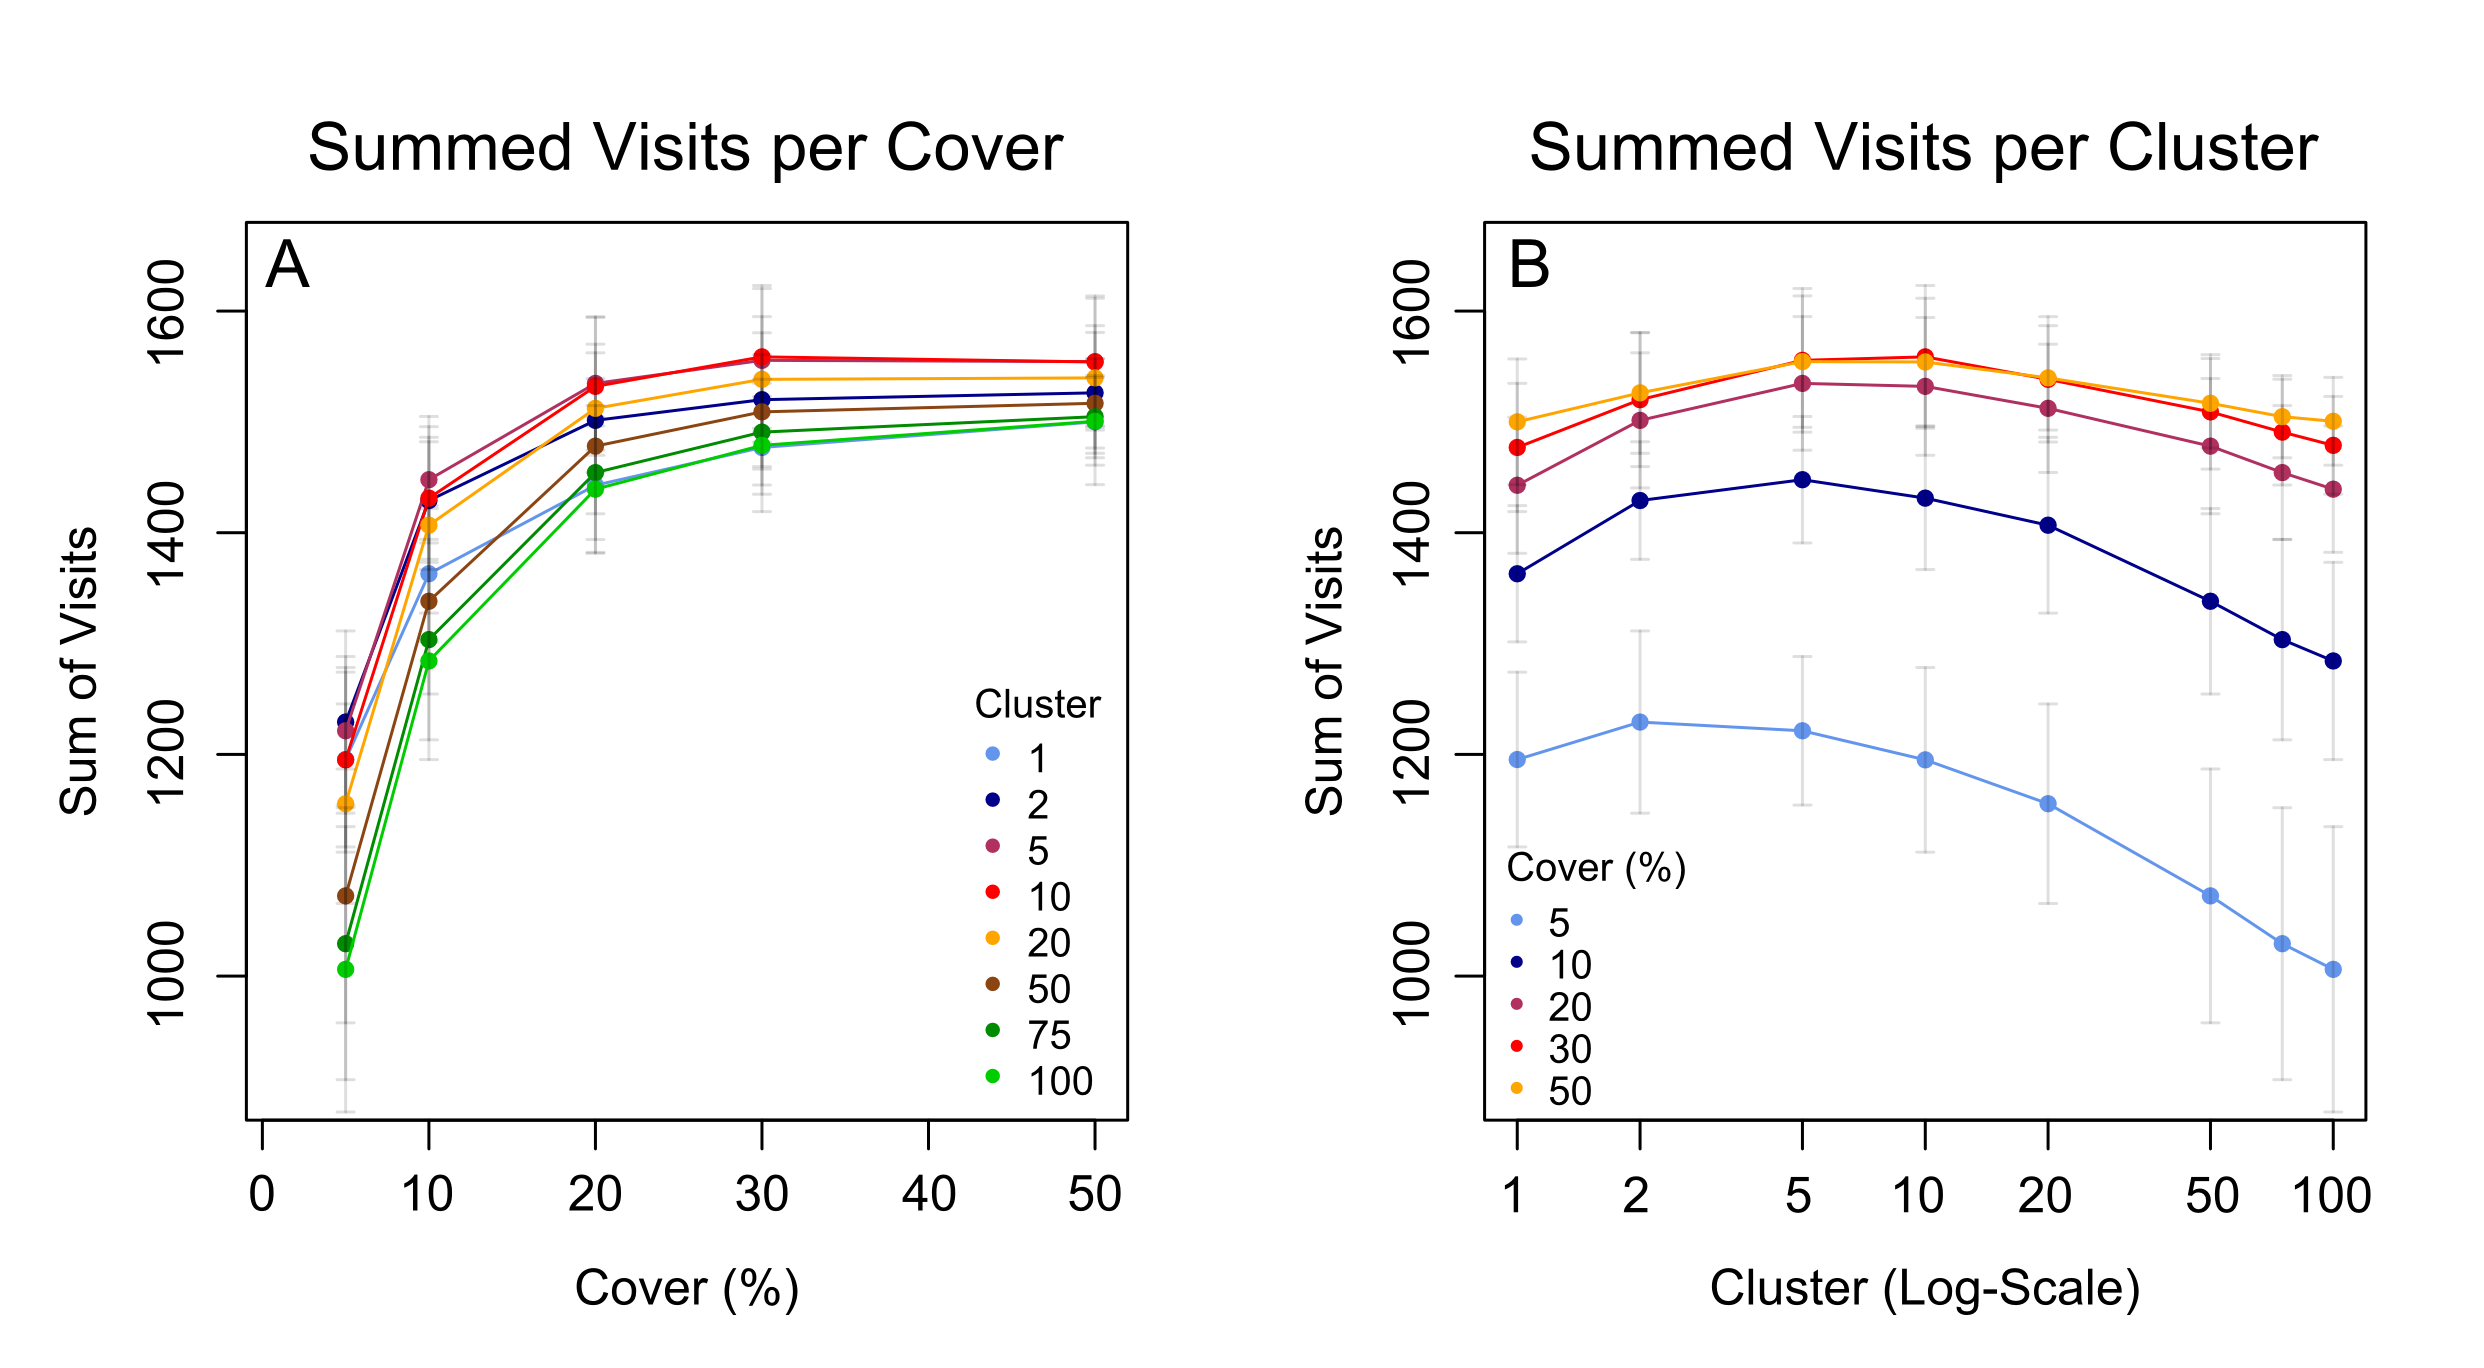
\includegraphics[width=14cm]{Images/nonfreq}
	\caption{Frequency independent influence of floral cover and degree of flower agglomeration on the summed visits within one simulation run. Cover strongly influences the number of visits as it reduces the flight and search time. Plot A shows a saturated relationship for all cluster values. This matches the Holling´s type II functional response. B) The degree of clustering also determines the sum of visits in a hump-shaped function. The maximum (depending on the cover) lays between 5 and 10 flowers per cluster. A small agglomeration of flowers reduces search times but keeps the next patch within short distance. The bigger the cluster, the more difficult to find the next one.}
	\label{fig:nonfreq}
\end{figure}

\clearpage

\begin{figure} [h!]
	\centering
	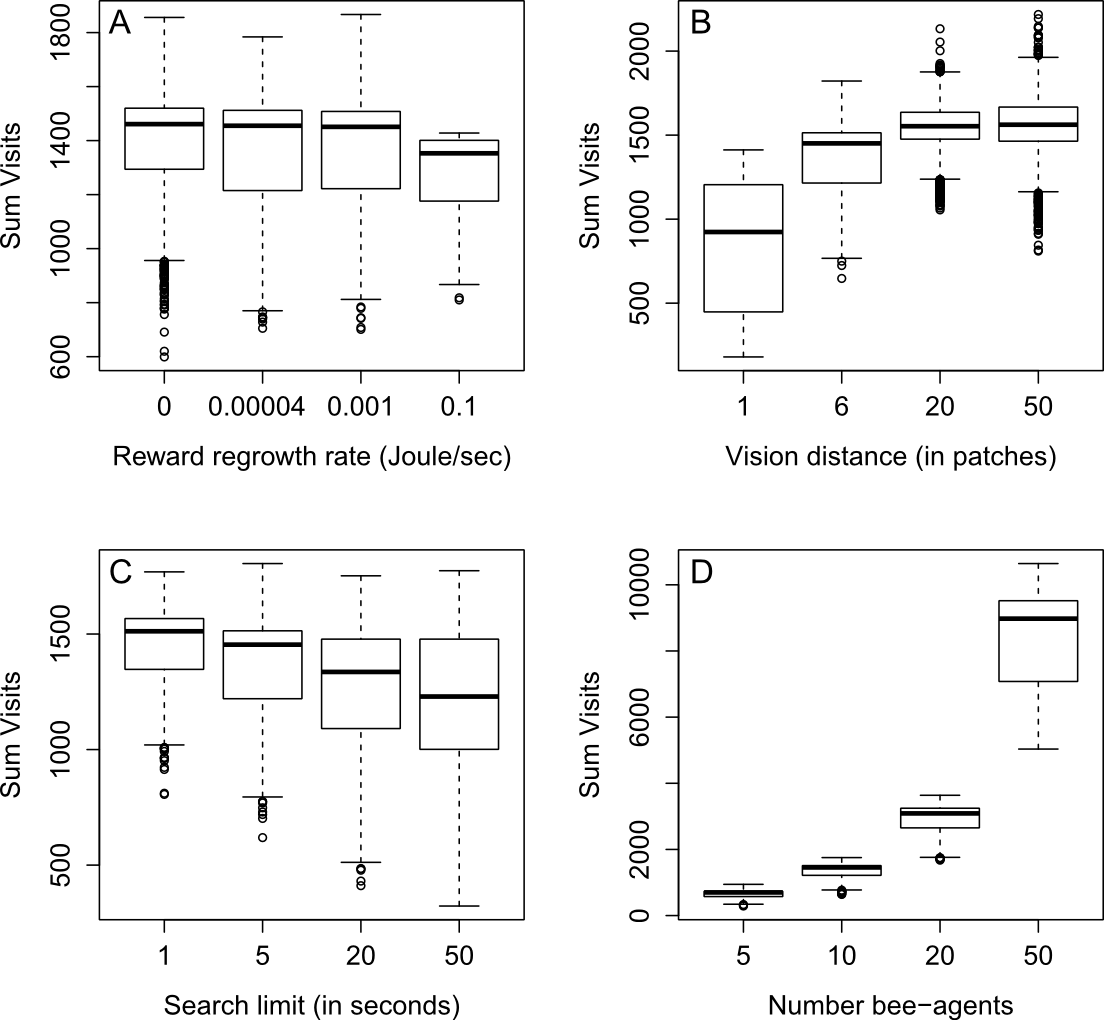
\includegraphics[width=14cm]{Images/SA_SUM}
	\caption{The influence of reward regrowth, vision, search limit and number of bee-agents on the total visits within a 1000 tick simulation run. A) Only an unnatural high reward regrowth has a small negative influence on the visits. B) Bee-agents with a far field of view can detect flowers faster, move in a direct way towards them and be therefore more efficient. However, the curve is saturated at a view of 20 patches. C) An increase in search time limit decreases the sum of visits and spread the variance. Bees-agents will keep searching for rare flowers instead of switching to the common species. D) As assumed, more bees lead to more visits.} 
	\label{fig:SA_SUM}
\end{figure}

\clearpage

\begin{figure} [!h] %
	\centering
	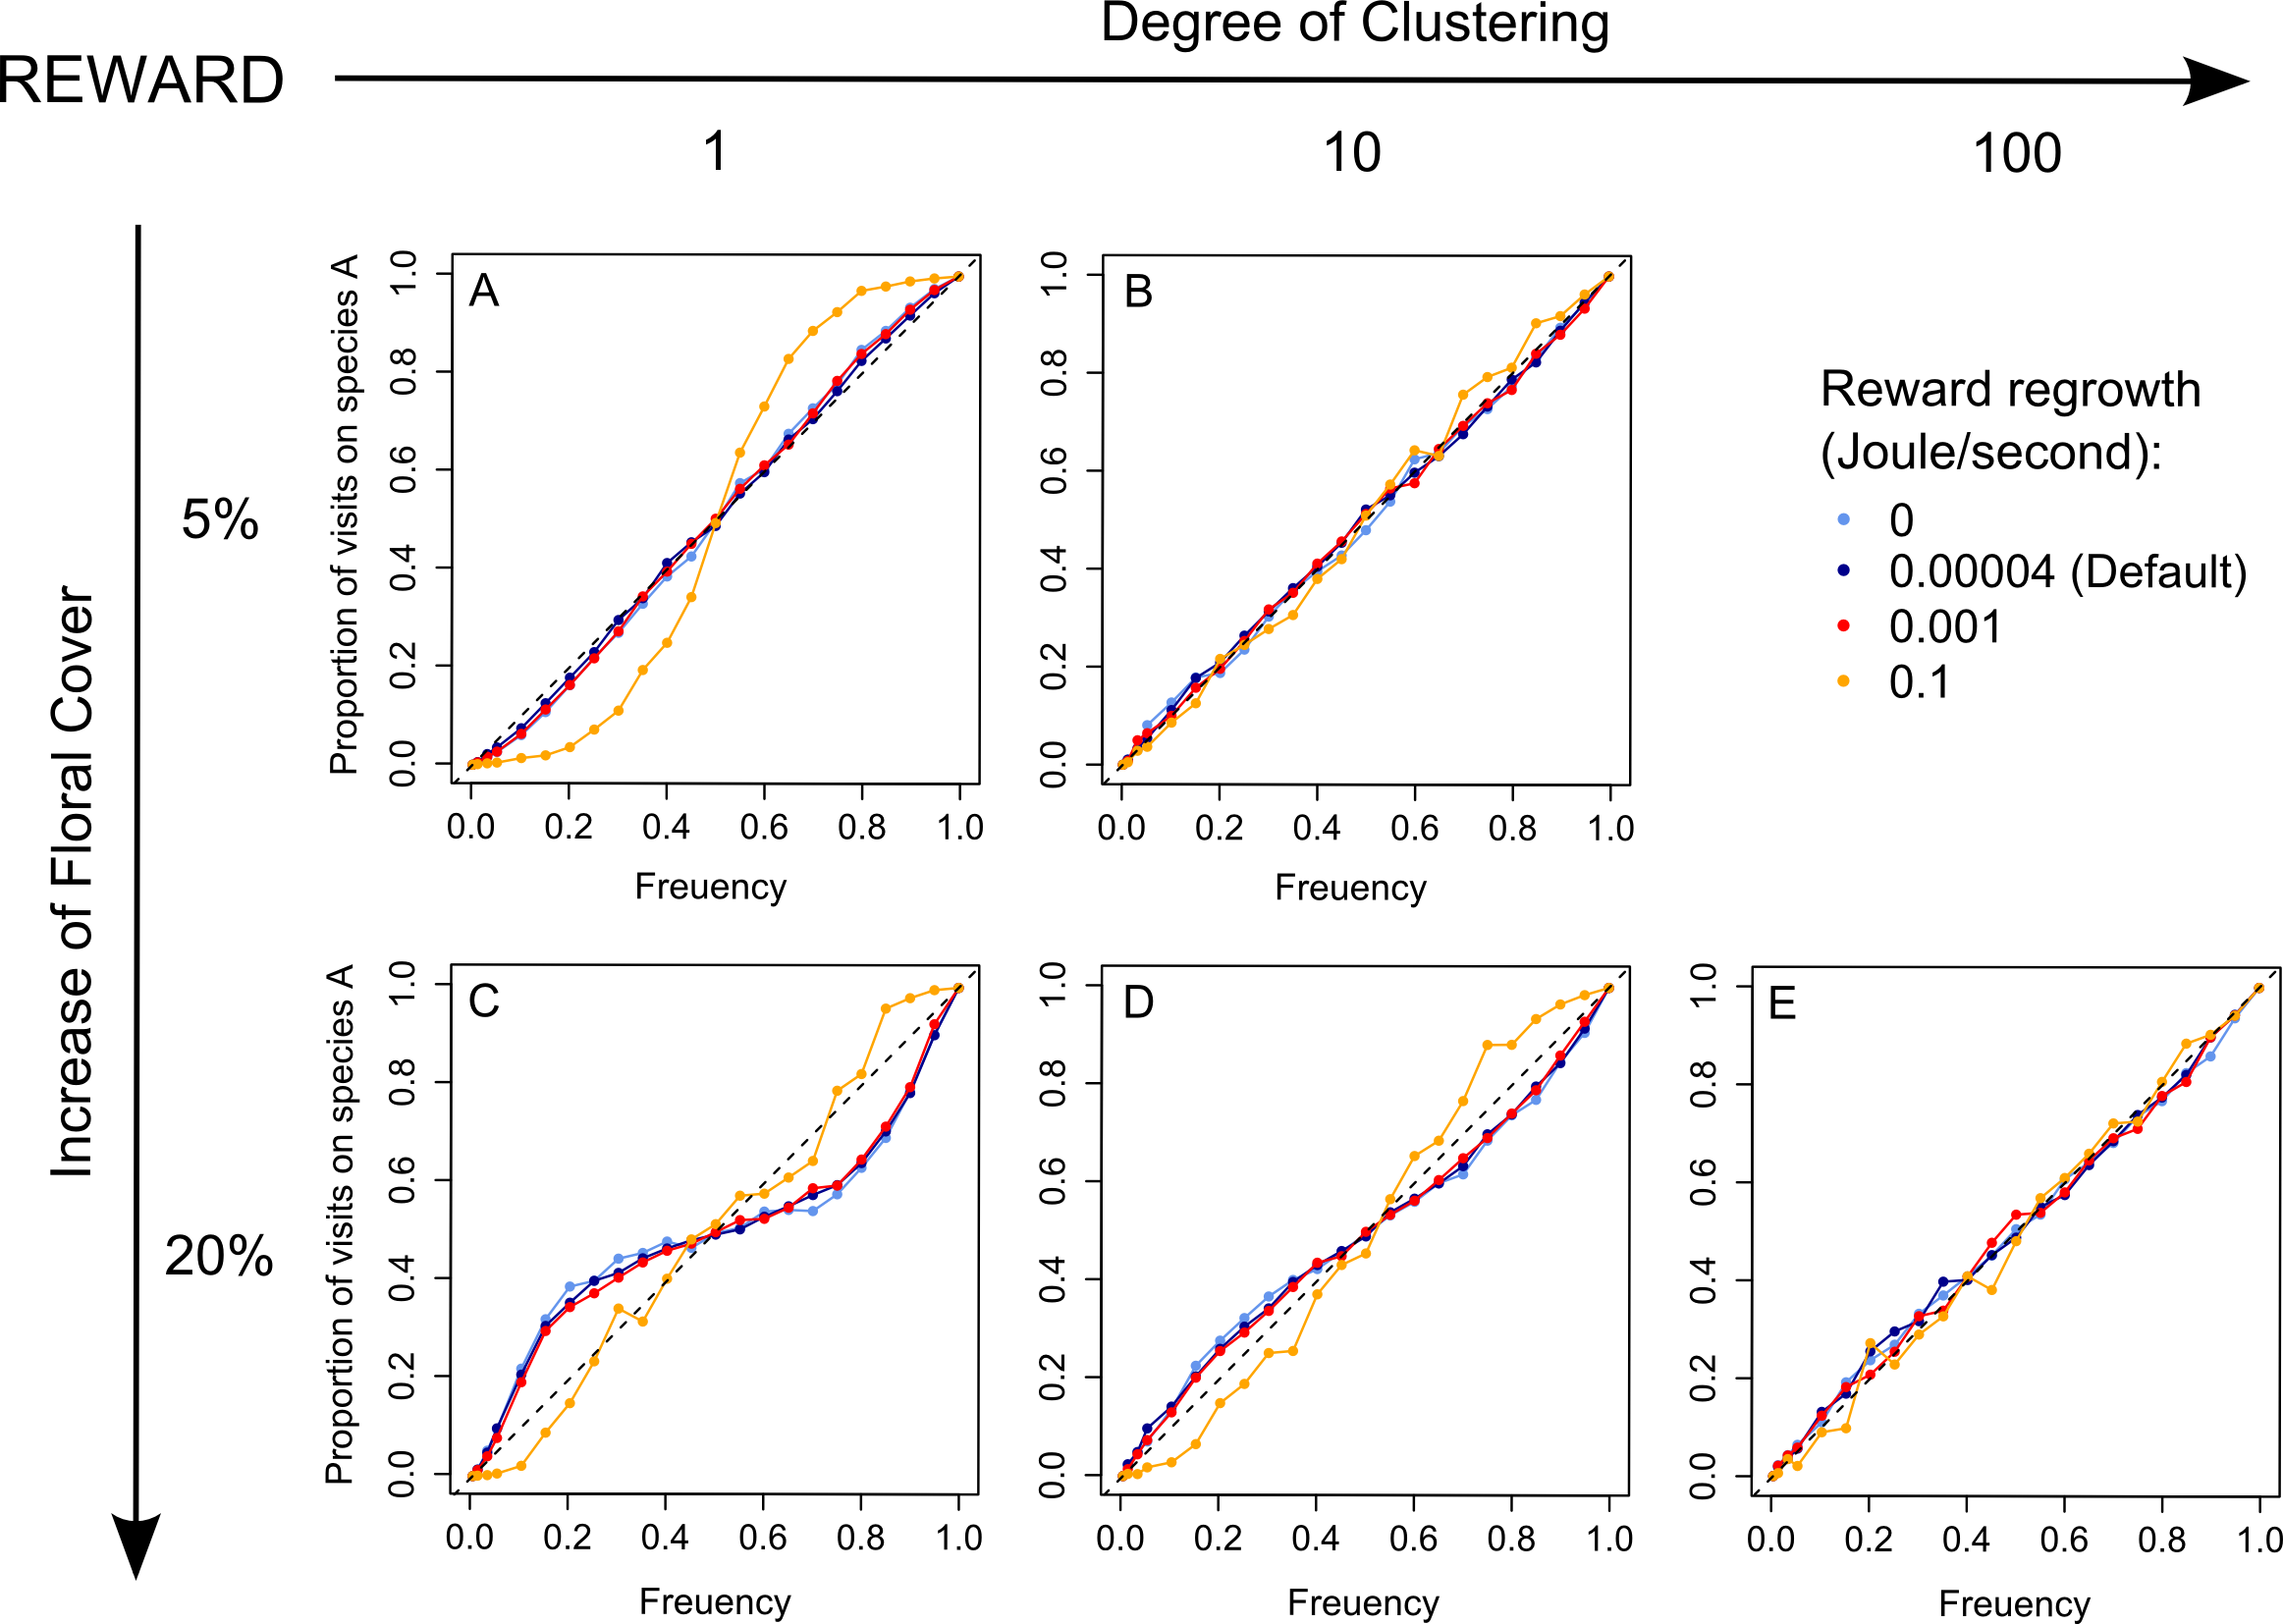
\includegraphics[width=14cm]{Images/SA_reward}
	\caption{Outcome of the model if the reward regrowth function is changed to 0, 0.004, 0.001 and 0.1 Joules per second. Only the unnatural high reward function (complete regrowth after 10 seconds) has an influence on the frequency dependence: the bee-agents have no more reason to change preference due to bad reward gained. This favors the more common species as shown in the opposite curving for no-cluster environments. A lower regrowth rate has no effect.} 
	\label{fig:SA_reward}
\end{figure}

\clearpage


\begin{figure} [!h]
	\centering
	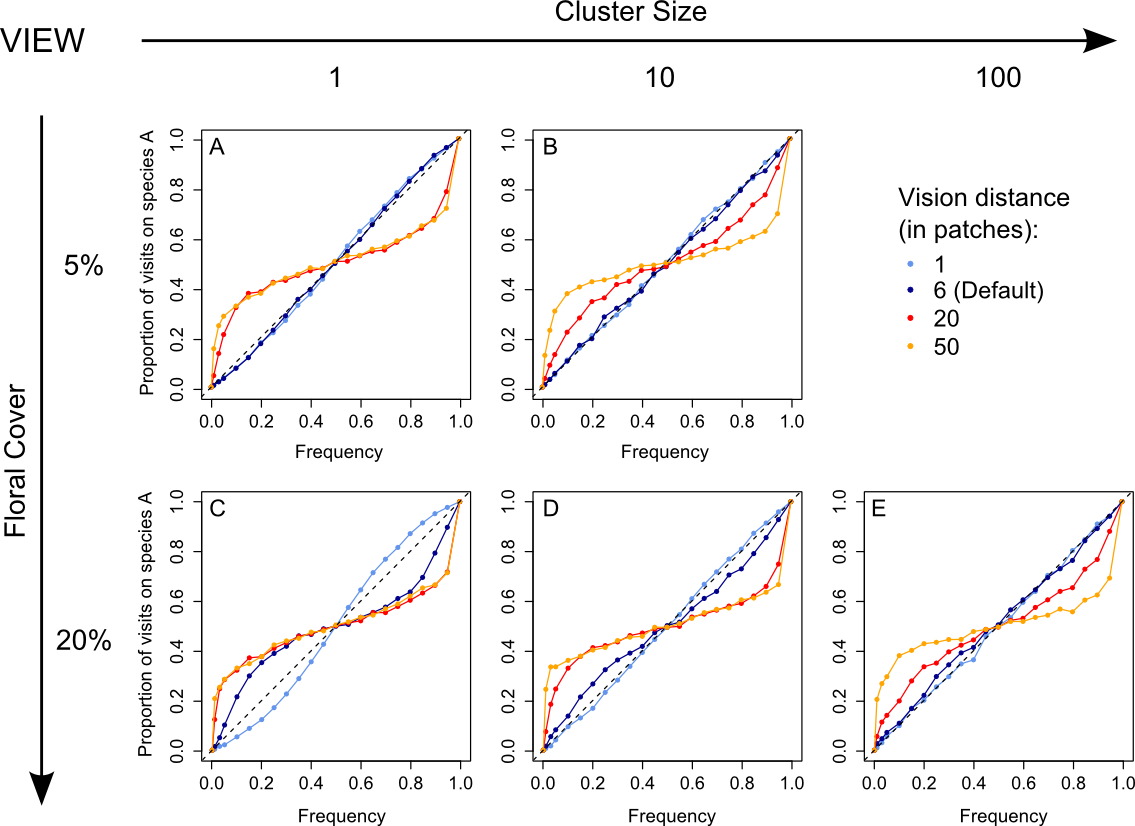
\includegraphics[width=14cm]{Images/SA_view}
	\caption{Effect of increased or reduced vision for the bee-agent. The vision influences the behavior of the bee-agent. If sees far, it can move on direct way towards the next preferred flower and saves searching time. But it also more often fly longer distances instead of changing to the common species. A high vision therefore increases the frequency dependence and a very low vision shifts the advantage towards the more abundant species.}
	\label{fig:SA_view}
\end{figure}

\clearpage


\begin{figure} [!h] 
	\centering
	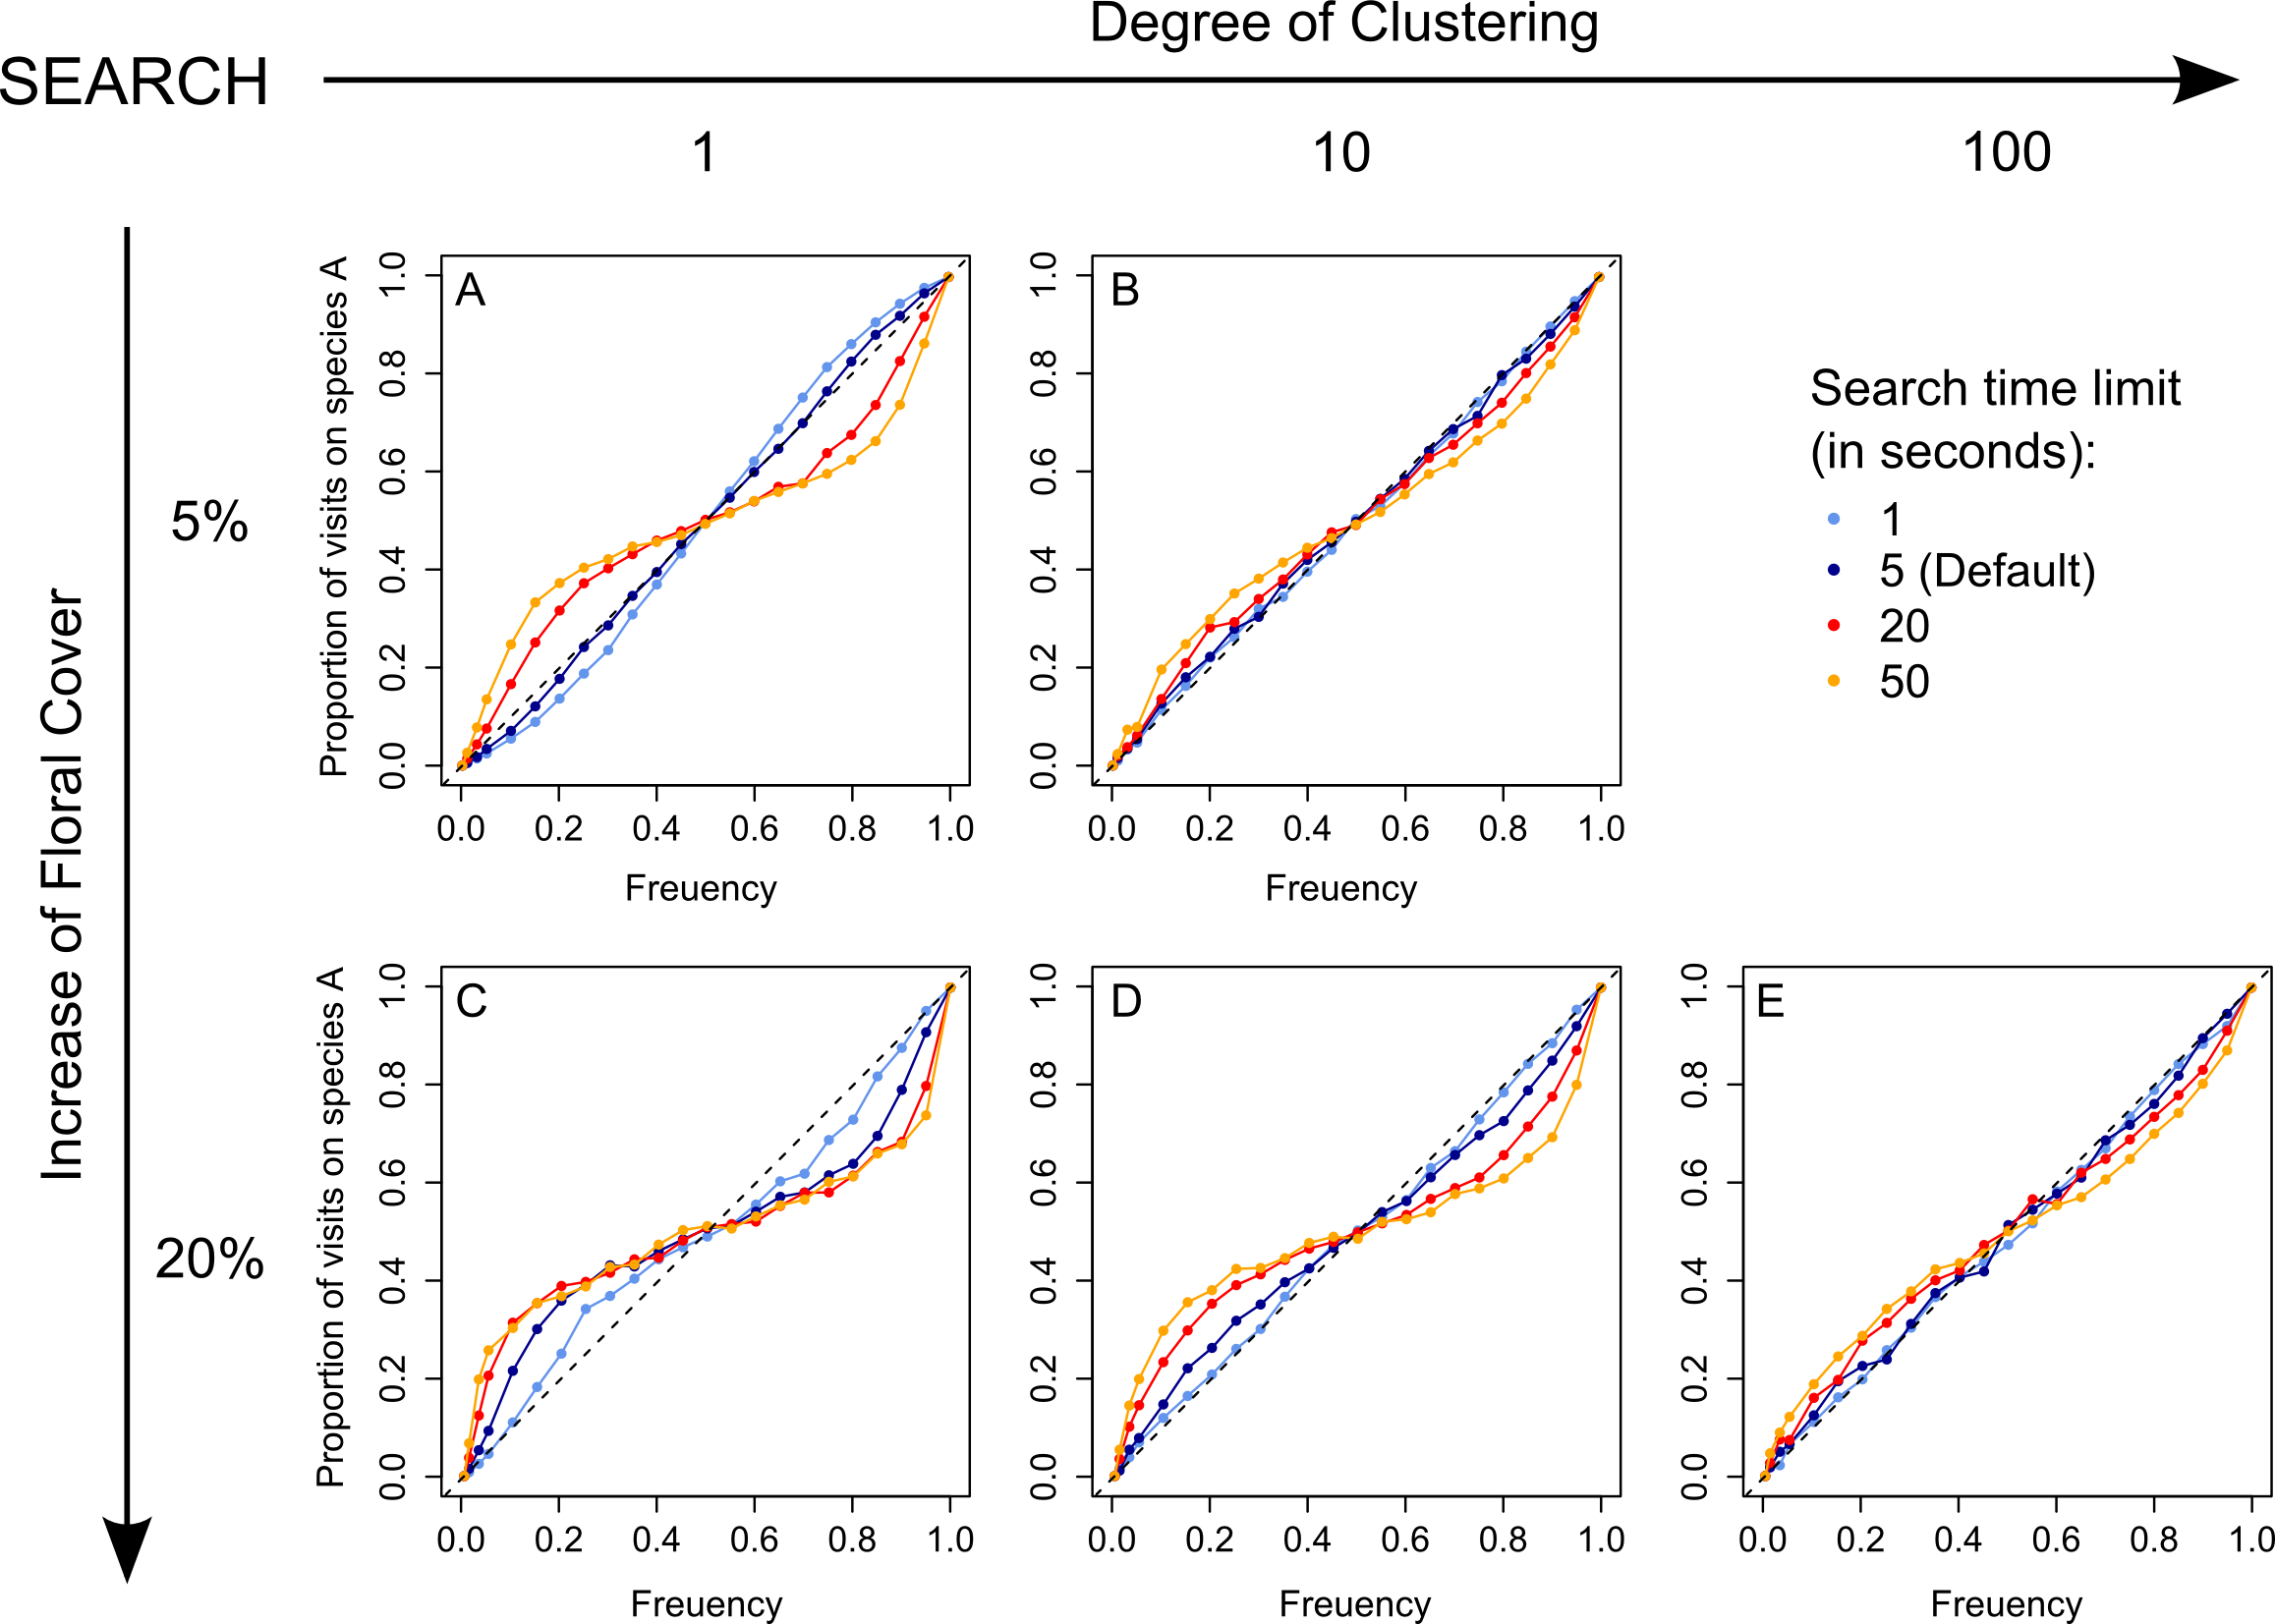
\includegraphics[width=14cm]{Images/SA_flight}
	\caption{Sensitivity analysis for search limits of 1,5, 20 and 50 seconds. The search limit is the number of seconds within a bee-agent searches for a unvisited and preferred flower, moving around the meadow by a correlated random walk. After the search limit is reached, the probability to change its flower preference increases with every additional second of unsuccessful search. The search limit has a similar effect on the outcome of the model as the vision because it also influences the change probability. With a higher search time, the bee-agent continues searing instead of switching to the more abundant flower, the frequency dependence is increased. A higher cluster value weakens the effect.}
	\label{fig:SA_flight}
\end{figure}

\clearpage

\begin{figure} [!h]
	\centering
	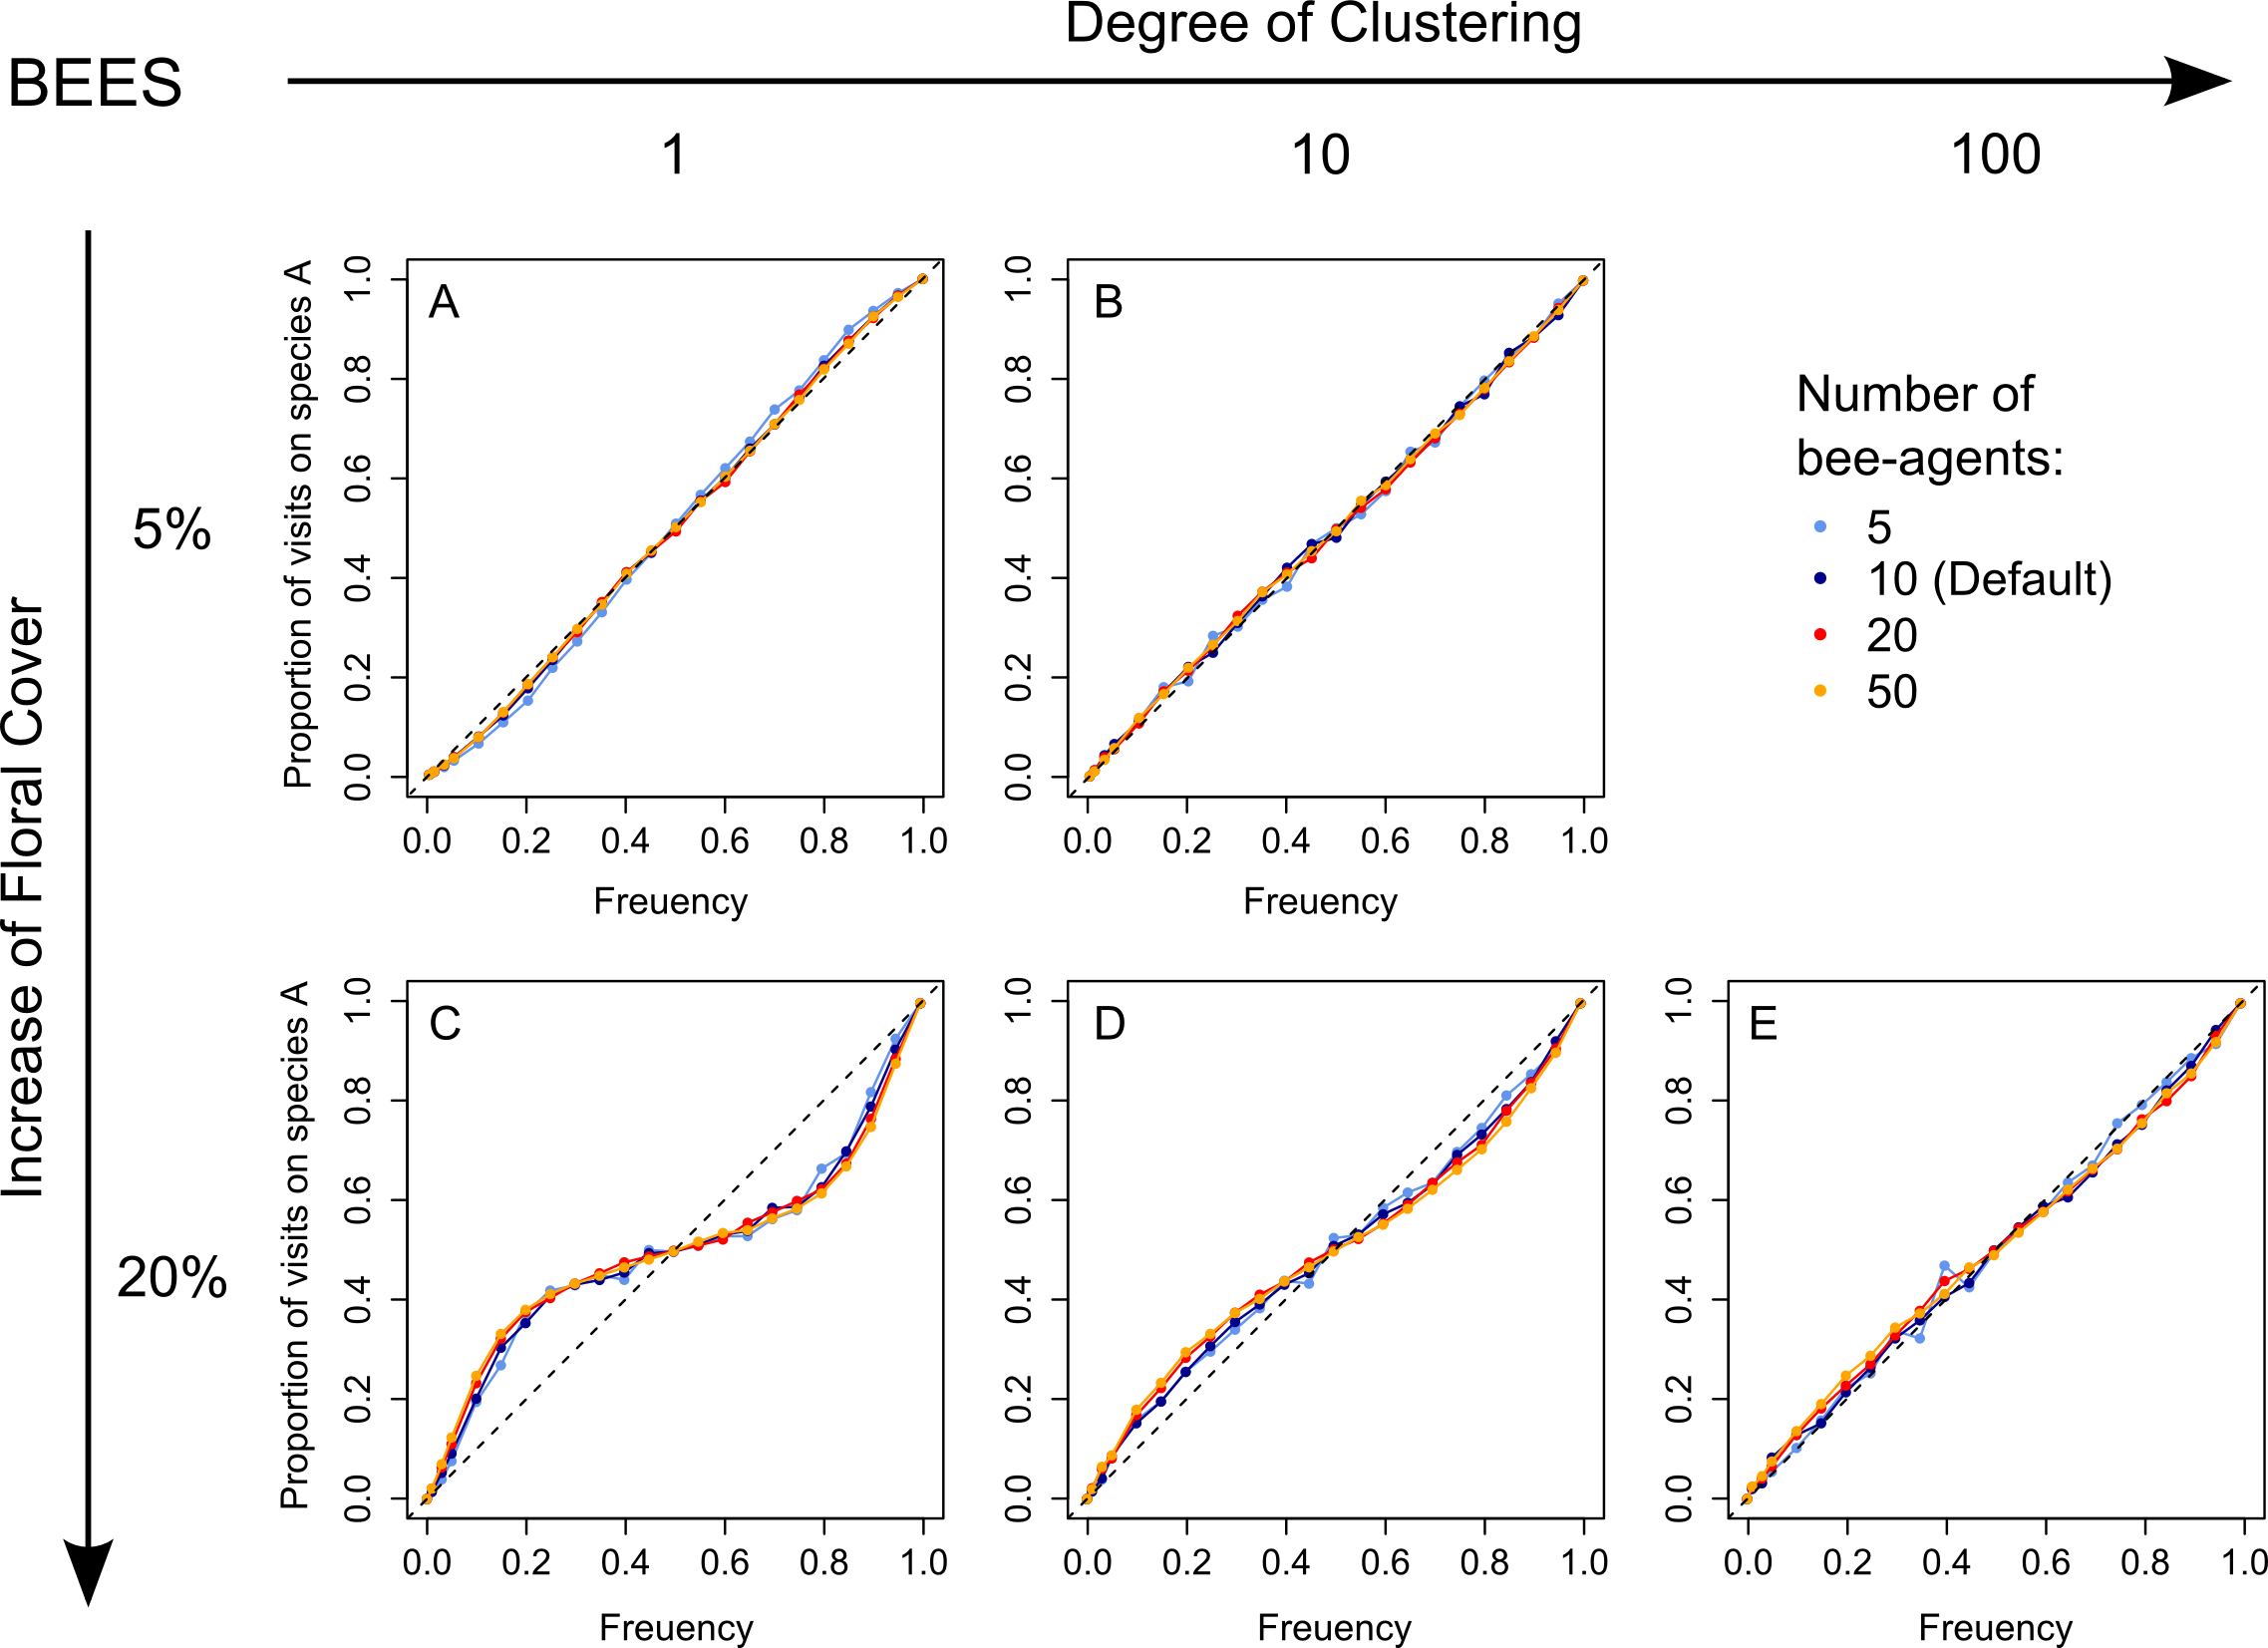
\includegraphics[width=14cm]{Images/SA_bees}
	\caption{Results of the model for 5, 10, 20 and 50 bee-agents on the meadow. The proportion of visits does not change, only the absolute numbers. Therefore has the pollinator density no influence on the frequency dependence.}
	\label{fig:SA_bees}
\end{figure}

%%%%%%%%%%%%%%%%%%%%%%%%%%%%%%%%%%%%%%%%%%%%%%%%%%%%%%%%%%%%%%%%%%%%%%%%



\newpage

\label{ch:code}

\section*{Code}

\lstset{ %
	language=R,                     % the language of the code
	basicstyle=\scriptsize,       % the size of the fonts that are used for the code
	numbers=left,                   % where to put the line-numbers
	numberstyle=\tiny\color{gray},  % the style that is used for the line-numbers
	stepnumber=1,                   % the step between two line-numbers. If it's 1, each line
	% will be numbered
	numbersep=5pt,                  % how far the line-numbers are from the code
	backgroundcolor=\color{white},  % choose the background color. You must add \usepackage{color}
	showspaces=false,               % show spaces adding particular underscores
	showstringspaces=false,         % underline spaces within strings
	showtabs=false,                 % show tabs within strings adding particular underscores
	frame=single,                   % adds a frame around the code
	rulecolor=\color{black},        % if not set, the frame-color may be changed on line-breaks within not-black text (e.g. commens (green here))
	tabsize=2,                      % sets default tabsize to 2 spaces
	captionpos=b,                   % sets the caption-position to bottom
	breaklines=true,                % sets automatic line breaking
	breakatwhitespace=false,        % sets if automatic breaks should only happen at whitespace
	title=\lstname,                 % show the filename of files included with \lstinputlisting;
	% also try caption instead of title
	keywordstyle=\color{Blue},      % keyword style
	commentstyle=\color{Gray},   % comment style
	stringstyle=\color{OliveGreen},      % string literal style
	escapeinside={\%*}{*)},         % if you want to add a comment within your code
	morekeywords={},            % if you want to add more keywords to the set
	deletendkeywords={sub, c, seq,mean}, %,length, sub,mean, sd, c
	otherkeywords={!,!=,~,,*,\&,\%/\%,\%*\%,\%\%,,,_,/},
	deletekeywords={SUB, SEQ, MEAN},
} 

\subsection*{Jena Analysis}
\lstinputlisting[language=R]{./jena.R}


\lstdefinelanguage{NetLogo}{
	morekeywords=[1]{to,to-report,end, extensions,to-report,globals,breed, patches-own,turtles-own, bees-own},
	extendedchars=true,
	breaklines=true,
	breakatwhitespace=true,
	basicstyle=\scriptsize,
	columns=fullflexible,
	tabsize=4,
	keywordstyle=[1]\color[rgb]{0.25,0.5,0.35},%\color[rgb]{0.4,0.8,0.2}\bfseries,
	morekeywords=[2]{let,set,loop, if, report, foreach, print, tick, while, every, ifelse, ask},
	keywordstyle=[2]\color{blue},
	alsoletter={-,?,.},
	morekeywords=[3]{position, not, reverse, fput, substring, length, word, timer,is-number?,filter,first, bf, butfirst, last, empty?, n-of, any?, color, who, patches, patch-here, member?, and, of, self, with, mean, sum,neighbors, shape, one-of, pcolor, round, with, count, myself, xcor, ycor, min-one-of, in-cone, random-normal, random-float, distance , fput, lput, but-last},
	keywordstyle=[3]\color{DarkOrchid},
	comment=[l]{\;},
	commentstyle=\color[rgb]{0.75,0.75,0.75},
	string=[d]{"},
	stringstyle=\color{orange},
	otherkeywords={<,>},
	morekeywords=[4]{1, 2, 3, 4, 5, 6, 7, 8, 9, 0, true, false},
	keywordstyle=[4]{\color{black}},
    }

\clearpage
\subsection*{NetLogo Model}
\lstinputlisting[language=NetLogo]{./bee_final.txt}


%\chapter*{Selbstständigkeitserklärung} % (in German!)

\vspace{2cm}

\section*{Erklärung}

Ich versichere hiermit, dass ich die vorliegende Arbeit ohne fremde Hilfe selbstständig verfasst und nur die angegebenen Quellen und Hilfsmittel benutzt habe. Wörtlich oder dem Sinn nach aus anderen Werken entnommene Stellen habe ich unter Angabe der Quellen kenntlich gemacht.

\medskip
\noindent (I hereby declare that I have composed this document unassistedly and that I only used the sources and devices I declared. Passages taken verbatim or in meaning from other sources are identified as such and the sources are acknowledged and cited.)

\vspace{2cm}

\noindent \year

\end{document}